% Options for packages loaded elsewhere
% Options for packages loaded elsewhere
\PassOptionsToPackage{unicode}{hyperref}
\PassOptionsToPackage{hyphens}{url}
\PassOptionsToPackage{dvipsnames,svgnames,x11names}{xcolor}
%
\documentclass[
  letterpaper,
  DIV=11,
  numbers=noendperiod]{scrreprt}
\usepackage{xcolor}
\usepackage{amsmath,amssymb}
\setcounter{secnumdepth}{5}
\usepackage{iftex}
\ifPDFTeX
  \usepackage[T1]{fontenc}
  \usepackage[utf8]{inputenc}
  \usepackage{textcomp} % provide euro and other symbols
\else % if luatex or xetex
  \usepackage{unicode-math} % this also loads fontspec
  \defaultfontfeatures{Scale=MatchLowercase}
  \defaultfontfeatures[\rmfamily]{Ligatures=TeX,Scale=1}
\fi
\usepackage{lmodern}
\ifPDFTeX\else
  % xetex/luatex font selection
\fi
% Use upquote if available, for straight quotes in verbatim environments
\IfFileExists{upquote.sty}{\usepackage{upquote}}{}
\IfFileExists{microtype.sty}{% use microtype if available
  \usepackage[]{microtype}
  \UseMicrotypeSet[protrusion]{basicmath} % disable protrusion for tt fonts
}{}
\makeatletter
\@ifundefined{KOMAClassName}{% if non-KOMA class
  \IfFileExists{parskip.sty}{%
    \usepackage{parskip}
  }{% else
    \setlength{\parindent}{0pt}
    \setlength{\parskip}{6pt plus 2pt minus 1pt}}
}{% if KOMA class
  \KOMAoptions{parskip=half}}
\makeatother
% Make \paragraph and \subparagraph free-standing
\makeatletter
\ifx\paragraph\undefined\else
  \let\oldparagraph\paragraph
  \renewcommand{\paragraph}{
    \@ifstar
      \xxxParagraphStar
      \xxxParagraphNoStar
  }
  \newcommand{\xxxParagraphStar}[1]{\oldparagraph*{#1}\mbox{}}
  \newcommand{\xxxParagraphNoStar}[1]{\oldparagraph{#1}\mbox{}}
\fi
\ifx\subparagraph\undefined\else
  \let\oldsubparagraph\subparagraph
  \renewcommand{\subparagraph}{
    \@ifstar
      \xxxSubParagraphStar
      \xxxSubParagraphNoStar
  }
  \newcommand{\xxxSubParagraphStar}[1]{\oldsubparagraph*{#1}\mbox{}}
  \newcommand{\xxxSubParagraphNoStar}[1]{\oldsubparagraph{#1}\mbox{}}
\fi
\makeatother

\usepackage{color}
\usepackage{fancyvrb}
\newcommand{\VerbBar}{|}
\newcommand{\VERB}{\Verb[commandchars=\\\{\}]}
\DefineVerbatimEnvironment{Highlighting}{Verbatim}{commandchars=\\\{\}}
% Add ',fontsize=\small' for more characters per line
\usepackage{framed}
\definecolor{shadecolor}{RGB}{241,243,245}
\newenvironment{Shaded}{\begin{snugshade}}{\end{snugshade}}
\newcommand{\AlertTok}[1]{\textcolor[rgb]{0.68,0.00,0.00}{#1}}
\newcommand{\AnnotationTok}[1]{\textcolor[rgb]{0.37,0.37,0.37}{#1}}
\newcommand{\AttributeTok}[1]{\textcolor[rgb]{0.40,0.45,0.13}{#1}}
\newcommand{\BaseNTok}[1]{\textcolor[rgb]{0.68,0.00,0.00}{#1}}
\newcommand{\BuiltInTok}[1]{\textcolor[rgb]{0.00,0.23,0.31}{#1}}
\newcommand{\CharTok}[1]{\textcolor[rgb]{0.13,0.47,0.30}{#1}}
\newcommand{\CommentTok}[1]{\textcolor[rgb]{0.37,0.37,0.37}{#1}}
\newcommand{\CommentVarTok}[1]{\textcolor[rgb]{0.37,0.37,0.37}{\textit{#1}}}
\newcommand{\ConstantTok}[1]{\textcolor[rgb]{0.56,0.35,0.01}{#1}}
\newcommand{\ControlFlowTok}[1]{\textcolor[rgb]{0.00,0.23,0.31}{\textbf{#1}}}
\newcommand{\DataTypeTok}[1]{\textcolor[rgb]{0.68,0.00,0.00}{#1}}
\newcommand{\DecValTok}[1]{\textcolor[rgb]{0.68,0.00,0.00}{#1}}
\newcommand{\DocumentationTok}[1]{\textcolor[rgb]{0.37,0.37,0.37}{\textit{#1}}}
\newcommand{\ErrorTok}[1]{\textcolor[rgb]{0.68,0.00,0.00}{#1}}
\newcommand{\ExtensionTok}[1]{\textcolor[rgb]{0.00,0.23,0.31}{#1}}
\newcommand{\FloatTok}[1]{\textcolor[rgb]{0.68,0.00,0.00}{#1}}
\newcommand{\FunctionTok}[1]{\textcolor[rgb]{0.28,0.35,0.67}{#1}}
\newcommand{\ImportTok}[1]{\textcolor[rgb]{0.00,0.46,0.62}{#1}}
\newcommand{\InformationTok}[1]{\textcolor[rgb]{0.37,0.37,0.37}{#1}}
\newcommand{\KeywordTok}[1]{\textcolor[rgb]{0.00,0.23,0.31}{\textbf{#1}}}
\newcommand{\NormalTok}[1]{\textcolor[rgb]{0.00,0.23,0.31}{#1}}
\newcommand{\OperatorTok}[1]{\textcolor[rgb]{0.37,0.37,0.37}{#1}}
\newcommand{\OtherTok}[1]{\textcolor[rgb]{0.00,0.23,0.31}{#1}}
\newcommand{\PreprocessorTok}[1]{\textcolor[rgb]{0.68,0.00,0.00}{#1}}
\newcommand{\RegionMarkerTok}[1]{\textcolor[rgb]{0.00,0.23,0.31}{#1}}
\newcommand{\SpecialCharTok}[1]{\textcolor[rgb]{0.37,0.37,0.37}{#1}}
\newcommand{\SpecialStringTok}[1]{\textcolor[rgb]{0.13,0.47,0.30}{#1}}
\newcommand{\StringTok}[1]{\textcolor[rgb]{0.13,0.47,0.30}{#1}}
\newcommand{\VariableTok}[1]{\textcolor[rgb]{0.07,0.07,0.07}{#1}}
\newcommand{\VerbatimStringTok}[1]{\textcolor[rgb]{0.13,0.47,0.30}{#1}}
\newcommand{\WarningTok}[1]{\textcolor[rgb]{0.37,0.37,0.37}{\textit{#1}}}

\usepackage{longtable,booktabs,array}
\newcounter{none} % for unnumbered tables
\usepackage{calc} % for calculating minipage widths
% Correct order of tables after \paragraph or \subparagraph
\usepackage{etoolbox}
\makeatletter
\patchcmd\longtable{\par}{\if@noskipsec\mbox{}\fi\par}{}{}
\makeatother
% Allow footnotes in longtable head/foot
\IfFileExists{footnotehyper.sty}{\usepackage{footnotehyper}}{\usepackage{footnote}}
\makesavenoteenv{longtable}
\usepackage{graphicx}
\makeatletter
\newsavebox\pandoc@box
\newcommand*\pandocbounded[1]{% scales image to fit in text height/width
  \sbox\pandoc@box{#1}%
  \Gscale@div\@tempa{\textheight}{\dimexpr\ht\pandoc@box+\dp\pandoc@box\relax}%
  \Gscale@div\@tempb{\linewidth}{\wd\pandoc@box}%
  \ifdim\@tempb\p@<\@tempa\p@\let\@tempa\@tempb\fi% select the smaller of both
  \ifdim\@tempa\p@<\p@\scalebox{\@tempa}{\usebox\pandoc@box}%
  \else\usebox{\pandoc@box}%
  \fi%
}
% Set default figure placement to htbp
\def\fps@figure{htbp}
\makeatother


% definitions for citeproc citations
\NewDocumentCommand\citeproctext{}{}
\NewDocumentCommand\citeproc{mm}{%
  \begingroup\def\citeproctext{#2}\cite{#1}\endgroup}
\makeatletter
 % allow citations to break across lines
 \let\@cite@ofmt\@firstofone
 % avoid brackets around text for \cite:
 \def\@biblabel#1{}
 \def\@cite#1#2{{#1\if@tempswa , #2\fi}}
\makeatother
\newlength{\cslhangindent}
\setlength{\cslhangindent}{1.5em}
\newlength{\csllabelwidth}
\setlength{\csllabelwidth}{3em}
\newenvironment{CSLReferences}[2] % #1 hanging-indent, #2 entry-spacing
 {\begin{list}{}{%
  \setlength{\itemindent}{0pt}
  \setlength{\leftmargin}{0pt}
  \setlength{\parsep}{0pt}
  % turn on hanging indent if param 1 is 1
  \ifodd #1
   \setlength{\leftmargin}{\cslhangindent}
   \setlength{\itemindent}{-1\cslhangindent}
  \fi
  % set entry spacing
  \setlength{\itemsep}{#2\baselineskip}}}
 {\end{list}}
\usepackage{calc}
\newcommand{\CSLBlock}[1]{\hfill\break\parbox[t]{\linewidth}{\strut\ignorespaces#1\strut}}
\newcommand{\CSLLeftMargin}[1]{\parbox[t]{\csllabelwidth}{\strut#1\strut}}
\newcommand{\CSLRightInline}[1]{\parbox[t]{\linewidth - \csllabelwidth}{\strut#1\strut}}
\newcommand{\CSLIndent}[1]{\hspace{\cslhangindent}#1}



\setlength{\emergencystretch}{3em} % prevent overfull lines

\providecommand{\tightlist}{%
  \setlength{\itemsep}{0pt}\setlength{\parskip}{0pt}}



 


\KOMAoption{captions}{tableheading}
\makeatletter
\@ifpackageloaded{bookmark}{}{\usepackage{bookmark}}
\makeatother
\makeatletter
\@ifpackageloaded{caption}{}{\usepackage{caption}}
\AtBeginDocument{%
\ifdefined\contentsname
  \renewcommand*\contentsname{Table of contents}
\else
  \newcommand\contentsname{Table of contents}
\fi
\ifdefined\listfigurename
  \renewcommand*\listfigurename{List of Figures}
\else
  \newcommand\listfigurename{List of Figures}
\fi
\ifdefined\listtablename
  \renewcommand*\listtablename{List of Tables}
\else
  \newcommand\listtablename{List of Tables}
\fi
\ifdefined\figurename
  \renewcommand*\figurename{Figure}
\else
  \newcommand\figurename{Figure}
\fi
\ifdefined\tablename
  \renewcommand*\tablename{Table}
\else
  \newcommand\tablename{Table}
\fi
}
\@ifpackageloaded{float}{}{\usepackage{float}}
\floatstyle{ruled}
\@ifundefined{c@chapter}{\newfloat{codelisting}{h}{lop}}{\newfloat{codelisting}{h}{lop}[chapter]}
\floatname{codelisting}{Listing}
\newcommand*\listoflistings{\listof{codelisting}{List of Listings}}
\makeatother
\makeatletter
\makeatother
\makeatletter
\@ifpackageloaded{caption}{}{\usepackage{caption}}
\@ifpackageloaded{subcaption}{}{\usepackage{subcaption}}
\makeatother
\usepackage{bookmark}
\IfFileExists{xurl.sty}{\usepackage{xurl}}{} % add URL line breaks if available
\urlstyle{same}
% fallback for those not using the hyperref driver hyperxmp:
\makeatletter
\@ifundefined{xmpquote}{\newcommand{\xmpquote}[1]{#1}}{}
\makeatother
\hypersetup{
  pdftitle={SUMO Tutorial},
  pdfauthor={유윤임},
  colorlinks=true,
  linkcolor={blue},
  filecolor={Maroon},
  citecolor={Blue},
  urlcolor={Blue},
  pdfcreator={LaTeX via pandoc}}


\title{SUMO Tutorial}
\author{유윤임}
\date{2026-10-04}
\begin{document}
\maketitle

\renewcommand*\contentsname{Table of contents}
{
\setcounter{tocdepth}{2}
\tableofcontents
}

\bookmarksetup{startatroot}

\chapter*{Preface}\label{preface}
\addcontentsline{toc}{chapter}{Preface}

\markboth{Preface}{Preface}

본 튜토리얼은 2026년 한양대학교에서 고준호 교수님이 강의하시는 교통공학
수업 중 SUMO 실습을 위해 작성되었습니다.

이 튜토리얼의 목적은 아래와 같습니다.

\begin{enumerate}
\def\labelenumi{\arabic{enumi}.}
\tightlist
\item
  SUMO 설치하기
\item
  SUMO 프로그램의 python tool을 사용하기 위해 ANACONDA와 Python 설치하기
\item
  SUMO input, output 파일을 편집하기 위한 vscode 설치
\item
  간단한 교통 네트워크를 시뮬레이션 하여 SUMO 동작 방법 이해하기
\item
  SUMO python tool 동작시키기
\item
  SUMO 예시 프로젝트 보기
\end{enumerate}

이 튜토리얼은 윈도우를 기준으로 작성되었습니다. 2025년 강의 수강생 중
MAC 사용자가 있어, 해당 학생의 질문을 기준으로 MAC 설치 방법을
작성하였으나, 오류가 있을 수 있습니다. 양해해주시면 감사드리겠습니다.

튜토리얼 오류, 문의 사항 등을 아래의 주소로 메일 보내주시면
감사드리겠습니다.

문의 이메일 : yoonim98@hanyang.ac.kr

\bookmarksetup{startatroot}

\chapter{Intro : SUMO 소개}\label{intro-sumo-uxc18cuxac1c}

\href{https://eclipse.dev/sumo/}{SUMO} 프로그램은 독일 우주항공
센터(Deutsches Zentrum für Luft-und Raumfahrt)의 교통 시스템 연구원에서
개발한 오픈소스 교통 시뮬레이션 프로그램입니다.

SUMO는 Simulation of Urban MObility의 약어인데, 이 이름처럼 도로 교통,
대중교통, 멀티모달 통행, 보행자 교통, PM 등 다양한 도시 교통수단에 대해
시뮬레이션을 제공합니다. 또한, Window, Mac, Linux 등 3가지 운영체제에서
시뮬레이션을 수행할 수 있습니다.

또한, 개별 차량의 움직임을 차량 추종 모형을 적용하여 구현하는 마이크로
시뮬레이션입니다(Lopez et al. 2018).

SUMO를 통해서 교통 정책, 신호 체계 변경의 효과 등을 예측해 볼 수
있습니다. 그 밖에도, 차량의 오염원 배출량, 에너지 소비량 등도
시뮬레이션해 볼 수 있습니다.

\url{video/intro_coex.mp4}

\part{SUMO 환경 구성하기}

본 장에서 SUMO 환경을 구성하는 법을 아래와 같이 설명하였습니다.

\begin{enumerate}
\def\labelenumi{\arabic{enumi}.}
\tightlist
\item
  vs code 설치
\item
  miniconda 설치와 sumo python 환경 설정
\item
  sumo 설치
\end{enumerate}

본래, SUMO만 설치하여도 시뮬레이션을 할 수 있습니다. 다만, SUMO
프로그램은 Python tool set을 제공하고 있어, 이를 이용하기 위해서는
python이 필요합니다. 또한, SUMO의 입력과 출력 파일은 기본적으로 xml
형식으로 이루어져 있습니다. 이 xml 파일을 메모장으로 편집할 수 있지만,
vscode와 같은 편집기를 사용하면 보다 쉽게 편집하고, 볼 수 있습니다.
미래에 sumo를 응용하여 쓰게 될 때, python code 작성하거나, sumo python
tool 프로그램 사용할 때, vscode가 도움이 될 수 있습니다.

이에 vscode 설치 방법, miniconda 설치 방법을 함께 서술하였습니다. sumo만
필요한 경우, sumo 설치만 따라하셔도 괜찮습니다. 그리고 기존에 사용하시는
코드 편집기가 이미 존재하고, python도 설치되어 있다면, 해당 장을
생략하셔도 괜찮습니다.

설치 방법을 간략하게 작성하였는데, 보다 상세한 가이드라인이 필요한 경우,
구글 검색창에 \texttt{윈도우\ vscdoe\ 설치}와 같이 입력하시면 상세한
자료를 찾을 수 있습니다.

순수 python의 경우, 버전관리, 앞으로 설치할 python, 환경변수 설정 등이
복잡한 부분이 있어 miniconda를 설치하는 것으로 안내드립니다. miniconda는
가상 환경을 만들어, python을 이용할 수 있어 파이썬 버전관리, python path
관리 등의 문제를 덜 겪을 수 있습니다.

이와 별개로, 순수 python이 이미 설치되어 있고, python path가 설정되어
있다면, 이 miniconda를 설치하지 않으셔도 됩니다. 본 튜토리얼에서 sumo
conda 환경을 활성화하는 부분을 빼고 python을 사용하는 부분을 따라하시면
되기 때문입니다.

\chapter{VS CODE 설치 :
윈도우}\label{vs-code-uxc124uxce58-uxc708uxb3c4uxc6b0}

\begin{enumerate}
\def\labelenumi{\arabic{enumi}.}
\item
  \href{https://code.visualstudio.com/}{VS CODE} 접속, \textbf{Download
  for Windows} 클릭해서 설치파일 다운로드
  \pandocbounded{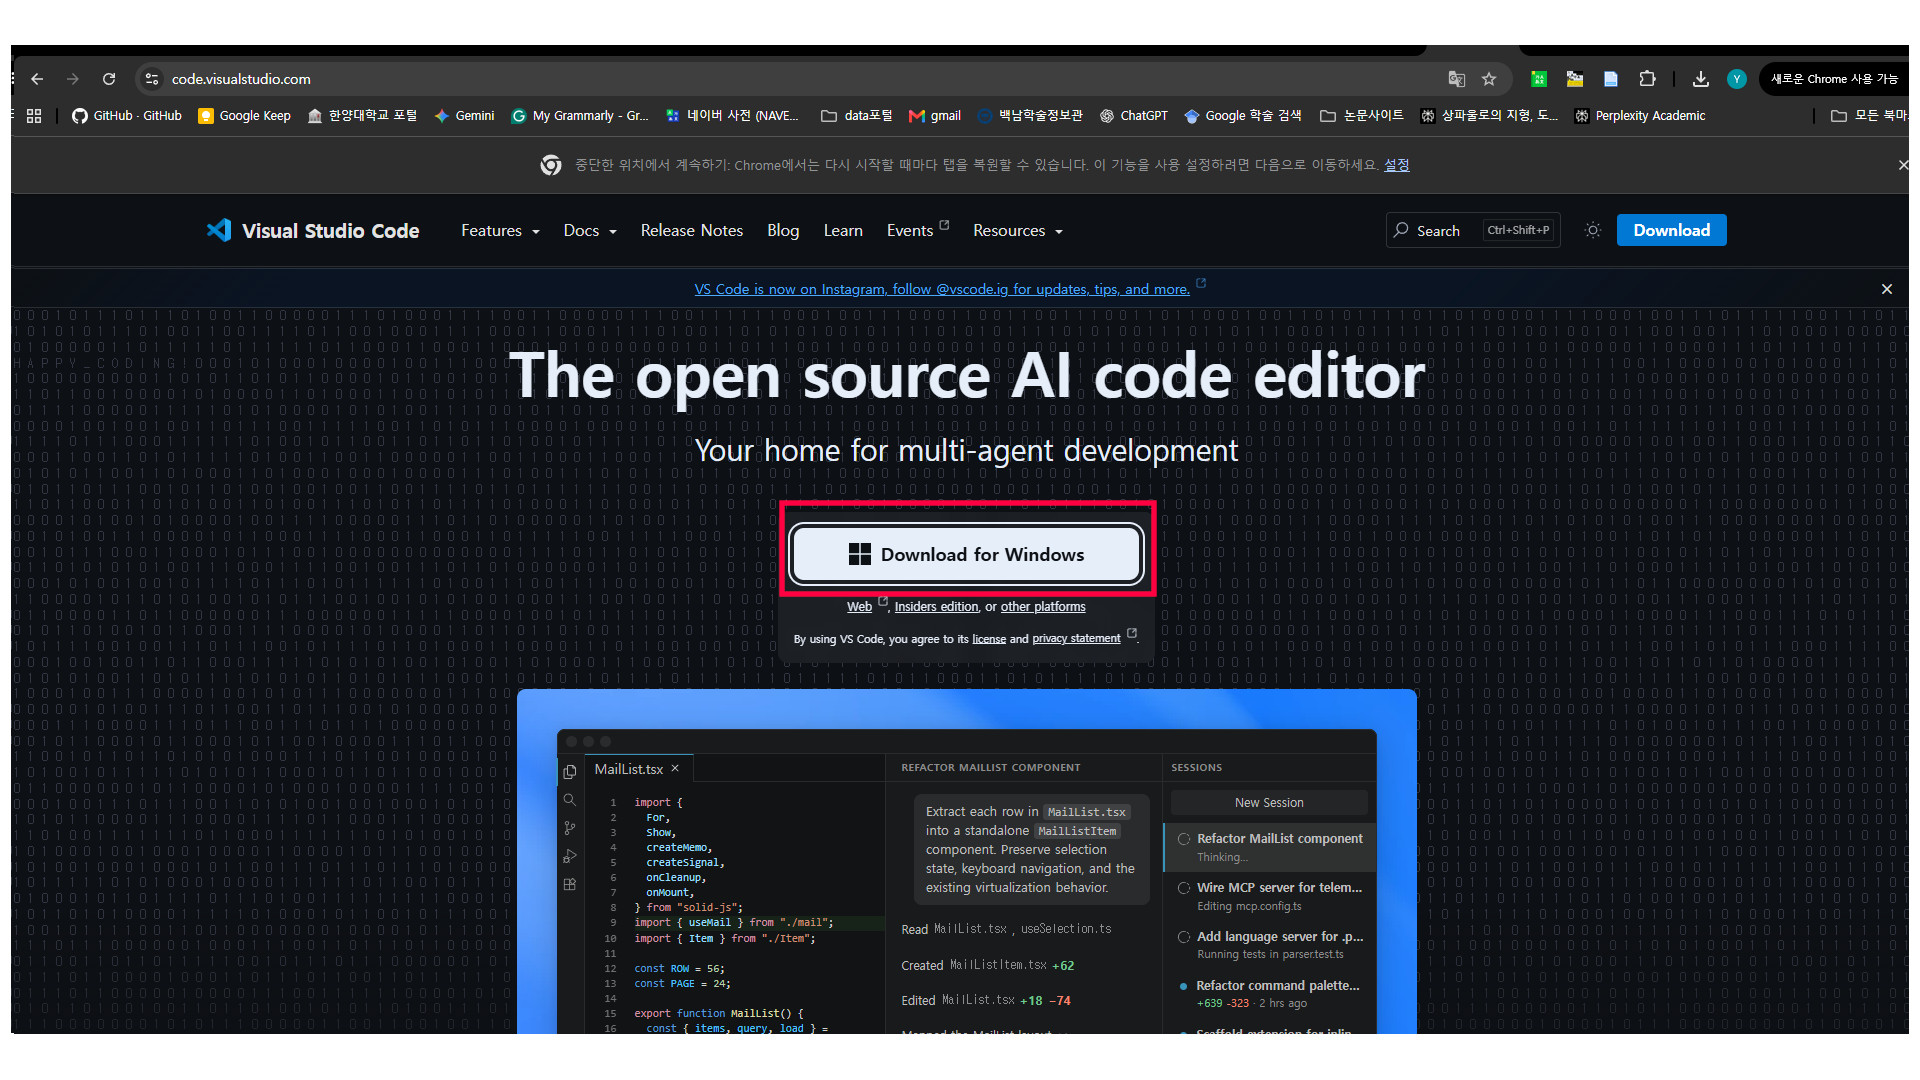
\includegraphics[keepaspectratio,alt={visual studio code main}]{image/install_window_visual_code_1.jpeg}}
\item
  설치파일 VSCodeUserSetup-x64\ldots exe 클릭.
\item
  라이센스 동의하기, Next 버튼 눌러서 진행, Default 세팅 유지
  \pandocbounded{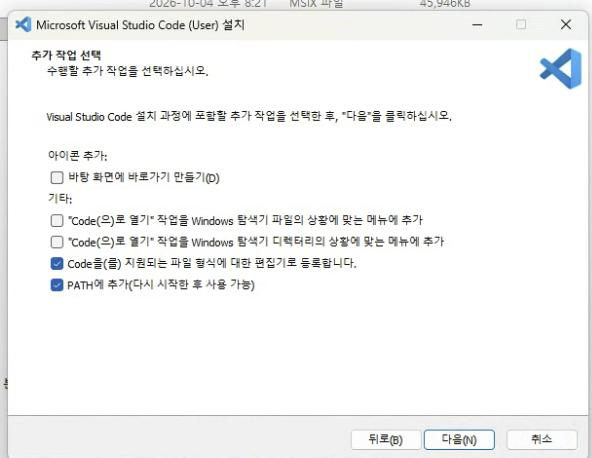
\includegraphics[keepaspectratio]{image/install_window_visual_code_2.jpeg}}
\item
  설치완료
  \pandocbounded{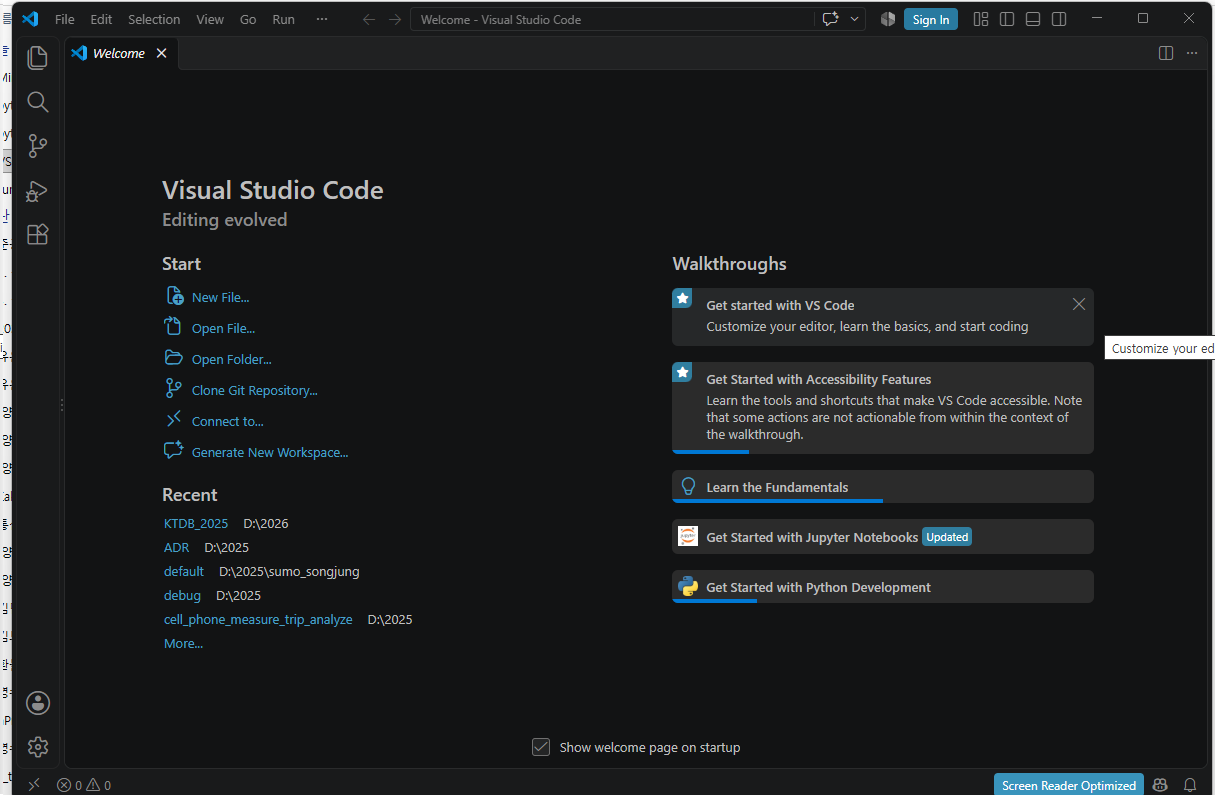
\includegraphics[keepaspectratio]{image/install_window_visual_code_3.png}}
\end{enumerate}

\chapter{Miniconda 설치 :
윈도우}\label{miniconda-uxc124uxce58-uxc708uxb3c4uxc6b0}

\section{Miniconda 설치}\label{miniconda-uxc124uxce58}

\begin{enumerate}
\def\labelenumi{\arabic{enumi}.}
\item
  \href{https://www.anaconda.com/download/success?reg=skipped-miniconda}{Miniconda
  Installer page} 접속 후, miniconda installer 다운로드
  \pandocbounded{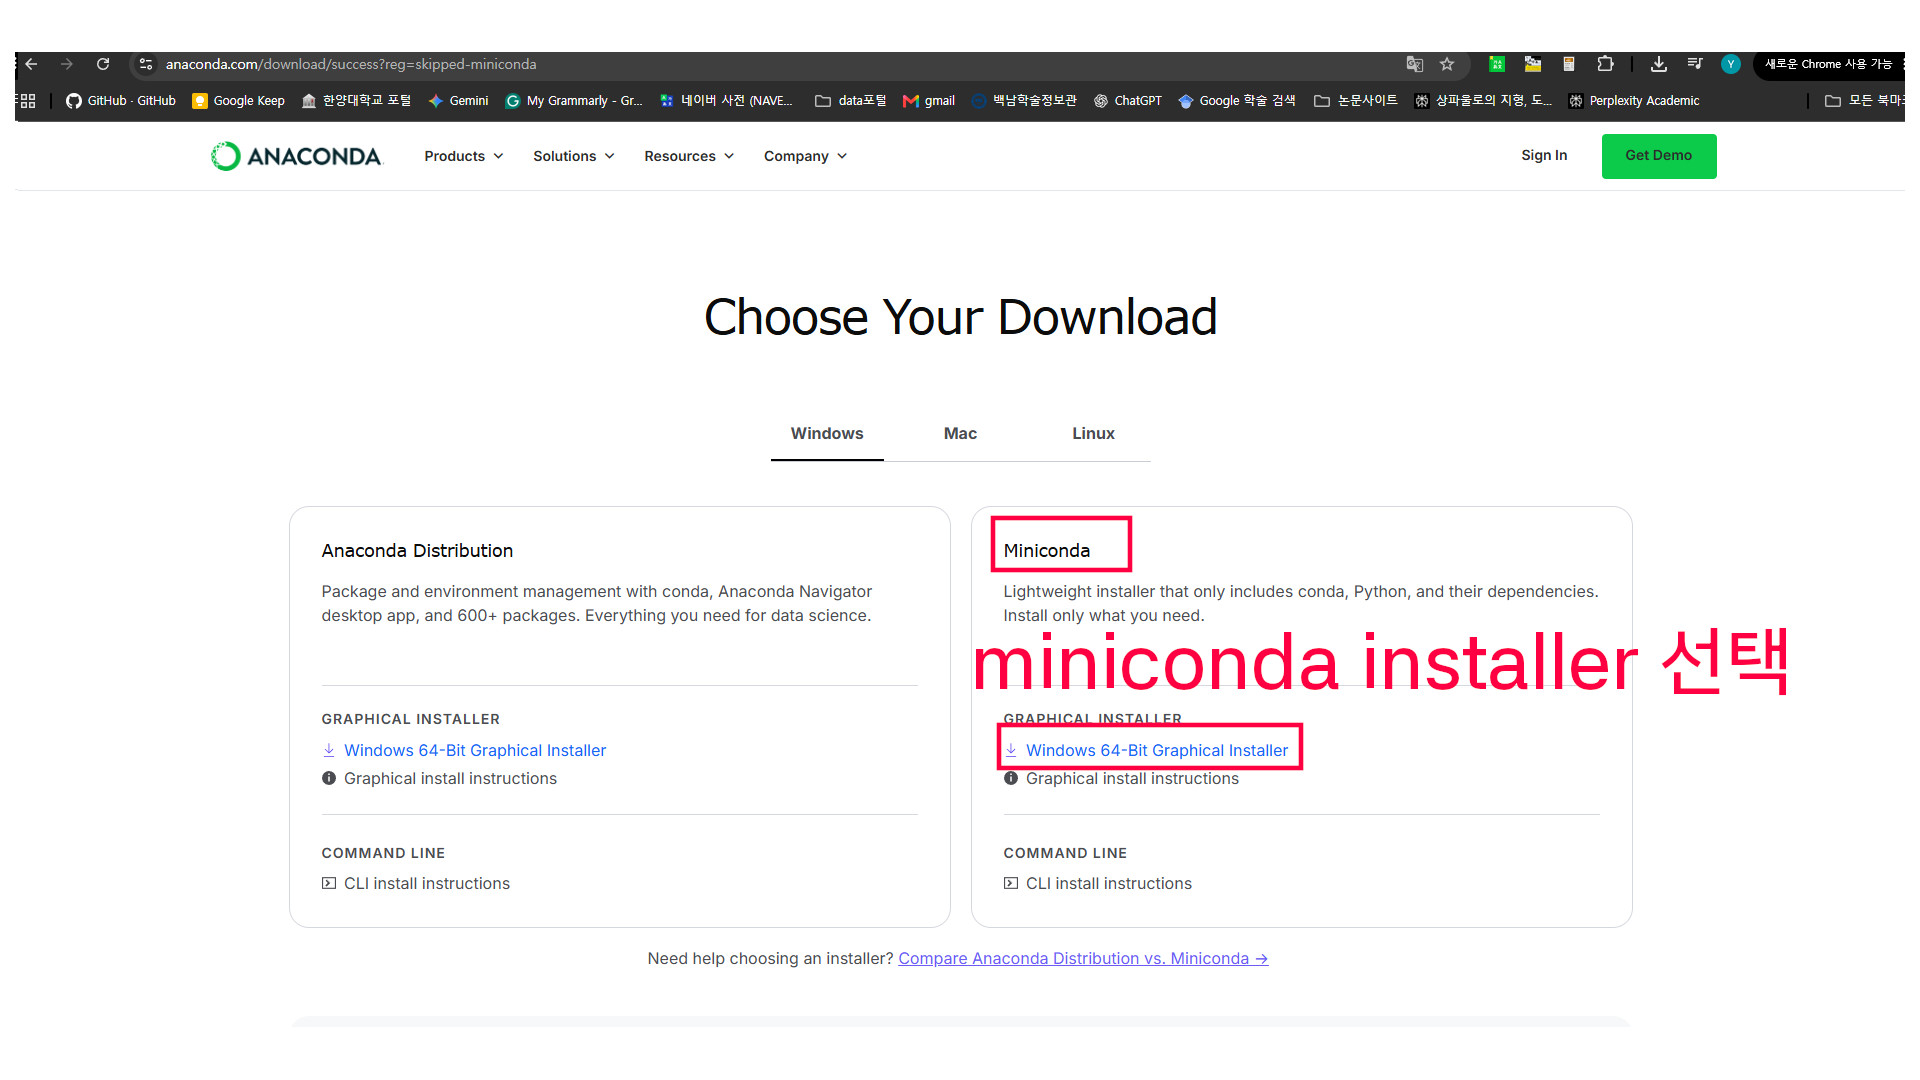
\includegraphics[keepaspectratio]{image/install_miniconda_1.jpeg}}
\item
  miniconda 설치파일을 열기, 아래의 그림과 지시사항에 따라 진행
\item
  Select Installation Type화면에서 All users 선택
\item
  Miniconda 설치 폴더 정하기

  \begin{itemize}
  \tightlist
  \item
    Destination 옆 설치폴더 정하기 버튼 클릭
  \item
    로컬디스크 C 선택
  \item
    새폴더만들기 선택
  \item
    새폴더 이름을 miniconda로 입력
  \item
    확인버튼 클릭
  \end{itemize}
\item
  Advanced Installation Option에서 Create shortcuts, Clear the package
  cache upon completion 체크 박스 선택
\item
  설치 완료 후, 윈도우 프로그램 창에서 anaconda prompt 찾아서 연 후,
  아래의 명령어 입력

  \begin{itemize}
  \tightlist
  \item
    이 작업을 하는 이유는 cmd 창에서 conda 명령어를 사용할 수 있게 하기
    위해서입니다.
  \end{itemize}

\begin{Shaded}
\begin{Highlighting}[]
\NormalTok{conda init cmd.exe}
\end{Highlighting}
\end{Shaded}

  \pandocbounded{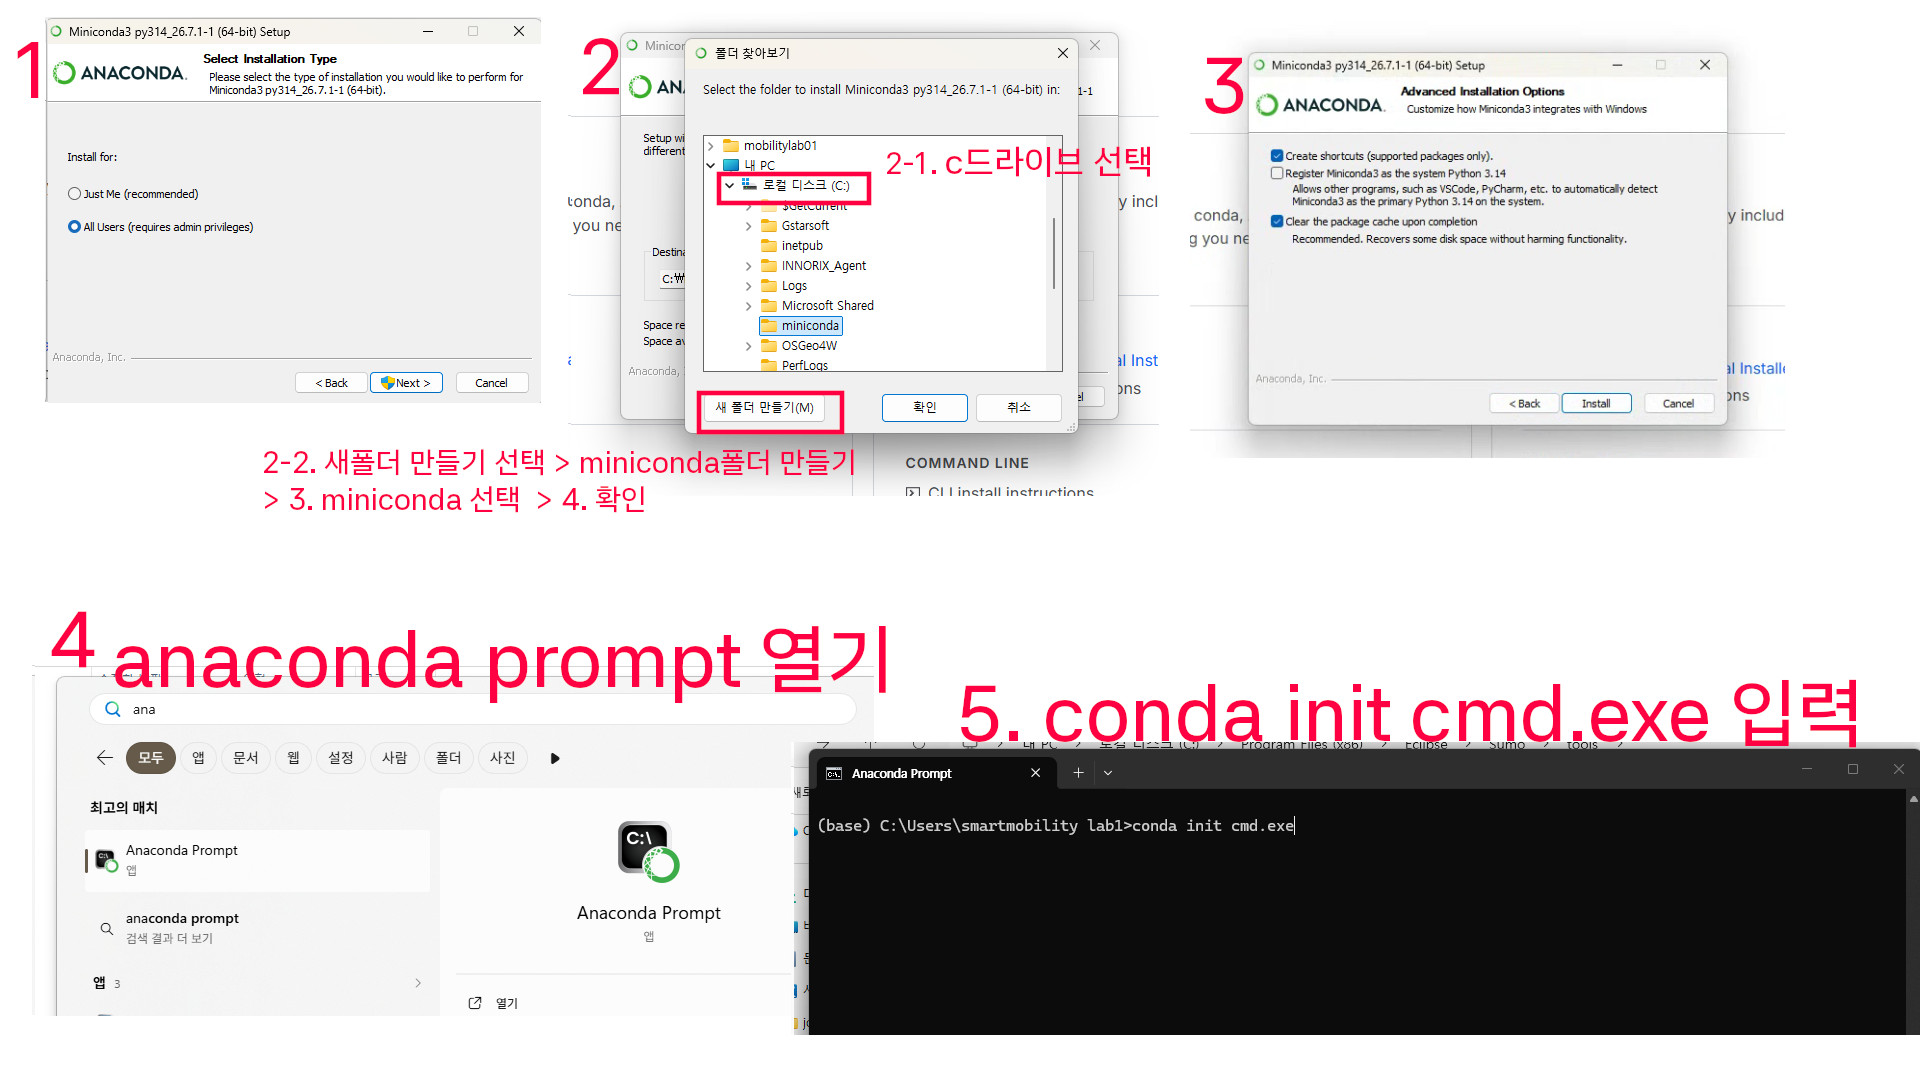
\includegraphics[keepaspectratio]{image/install_miniconda_2.jpeg}}
\item
  윈도우 프로그램 창에 cmd 입력, 관리자 권한으로 cmd 열기 클릭
\item
  cmd 창에 아래의 명령어 입력 후, 다음 명령줄 앞에 (base)가 아래 그림과
  같이 뜨면 miniconda 설치 성공
  \pandocbounded{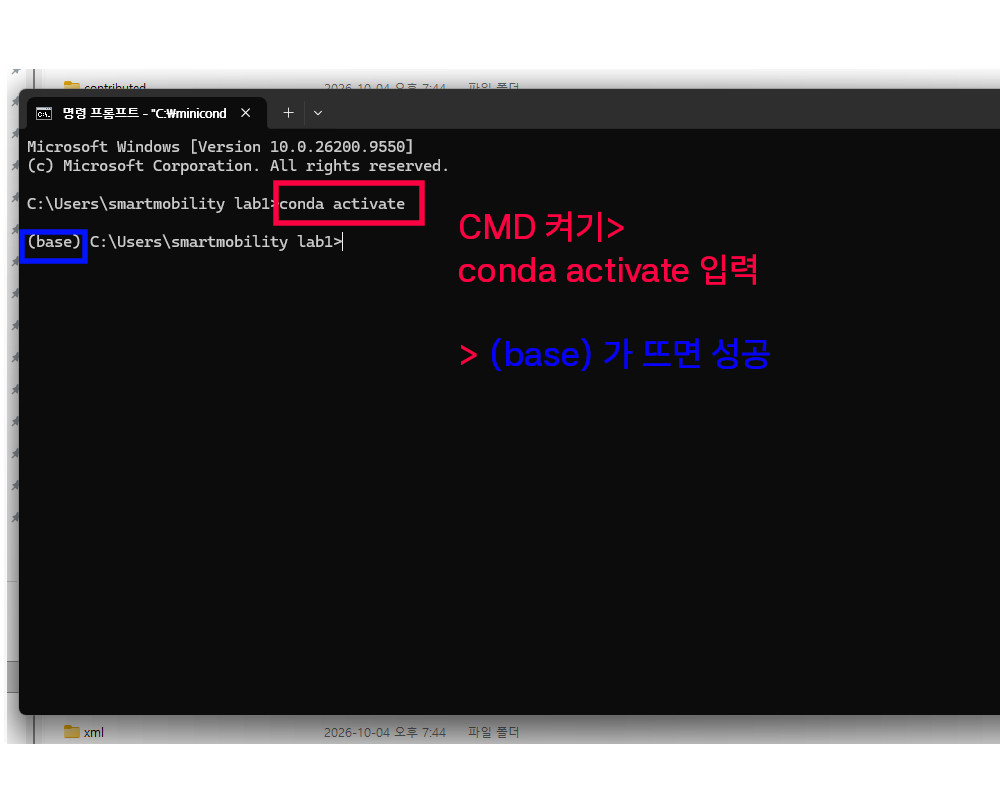
\includegraphics[keepaspectratio]{image/install_miniconda_3.jpeg}}
\end{enumerate}

\begin{center}\rule{0.5\linewidth}{0.5pt}\end{center}

\section{SUMO 콘다 파이썬 환경
만들기}\label{sumo-uxcf58uxb2e4-uxd30cuxc774uxc36c-uxd658uxacbd-uxb9ccuxb4e4uxae30}

\begin{enumerate}
\def\labelenumi{\arabic{enumi}.}
\item
  cmd 창 열기
\item
  sumo 전용 conda 환경을 만들기 위해 아래 명령어 입력

  \begin{itemize}
  \tightlist
  \item
    환경명 : sumopy
  \item
    파이썬 버전 : 3.11
  \item
    만약 파이썬 버전 3.11에서 sumo tool을 쓰는 데 문제가 생긴다면,
    3.7버전의 새로운 환경을 만들어서 사용하시면 됩니다.
  \end{itemize}

\begin{Shaded}
\begin{Highlighting}[]
\NormalTok{conda create }\AttributeTok{{-}n}\NormalTok{ sumopy python=3.11}
\end{Highlighting}
\end{Shaded}

  \pandocbounded{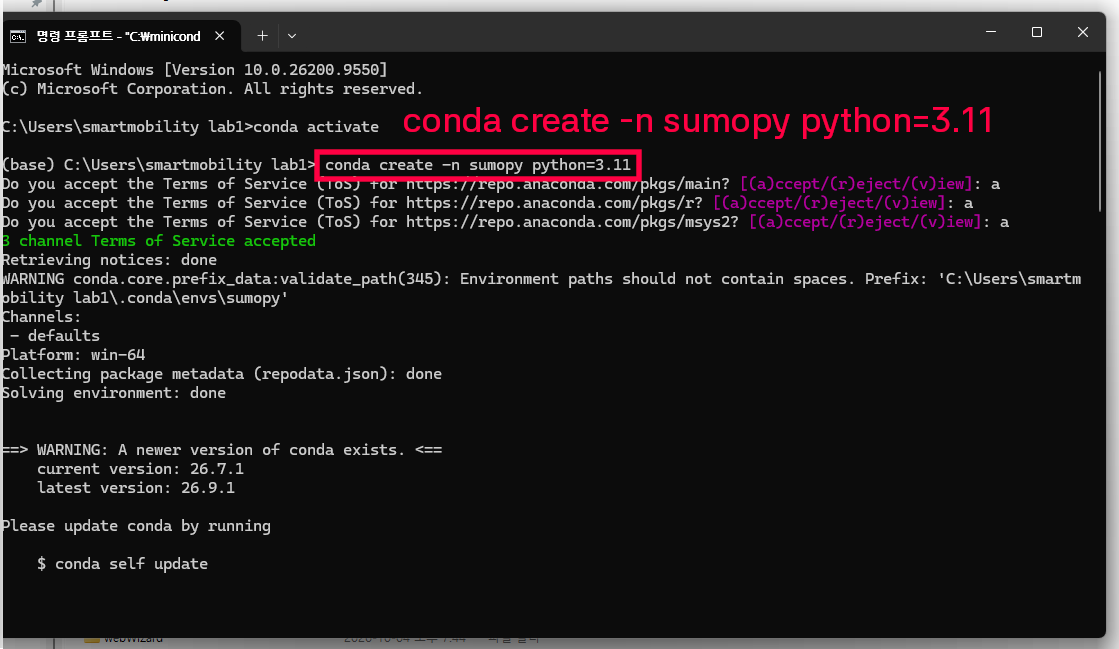
\includegraphics[keepaspectratio]{image/install_miniconda_4.png}}
\item
  명령어 입력하여 sumopy 활성화 하기

  \begin{itemize}
  \tightlist
  \item
    아래 명령어 입력 후, 나오는 다음 명령줄 앞에 (sumopy)가 나오면
    환경이 정상적으로 생성된 것입니다.
  \end{itemize}

\begin{Shaded}
\begin{Highlighting}[]
\NormalTok{conda activate sumopy}
\end{Highlighting}
\end{Shaded}
\item
  python 버전 확인하기

  \begin{itemize}
  \tightlist
  \item
    파이썬 버전이 나오면 환경에서 파이썬이 정상적으로 설치된 것입니다.
  \end{itemize}

\begin{Shaded}
\begin{Highlighting}[]
\NormalTok{python {-}}\AttributeTok{{-}version}
\end{Highlighting}
\end{Shaded}
\item
  아래 명령어를 입력하여, sumo python tools에 필요한 패키지 설치
\end{enumerate}

\begin{Shaded}
\begin{Highlighting}[]
\NormalTok{python }\AttributeTok{{-}m}\NormalTok{ pip install }\AttributeTok{{-}r} \StringTok{"}\PreprocessorTok{\%}\VariableTok{SUMO\_HOME}\PreprocessorTok{\%}\StringTok{\textbackslash{}tools\textbackslash{}requirements.txt"}
\end{Highlighting}
\end{Shaded}

\pandocbounded{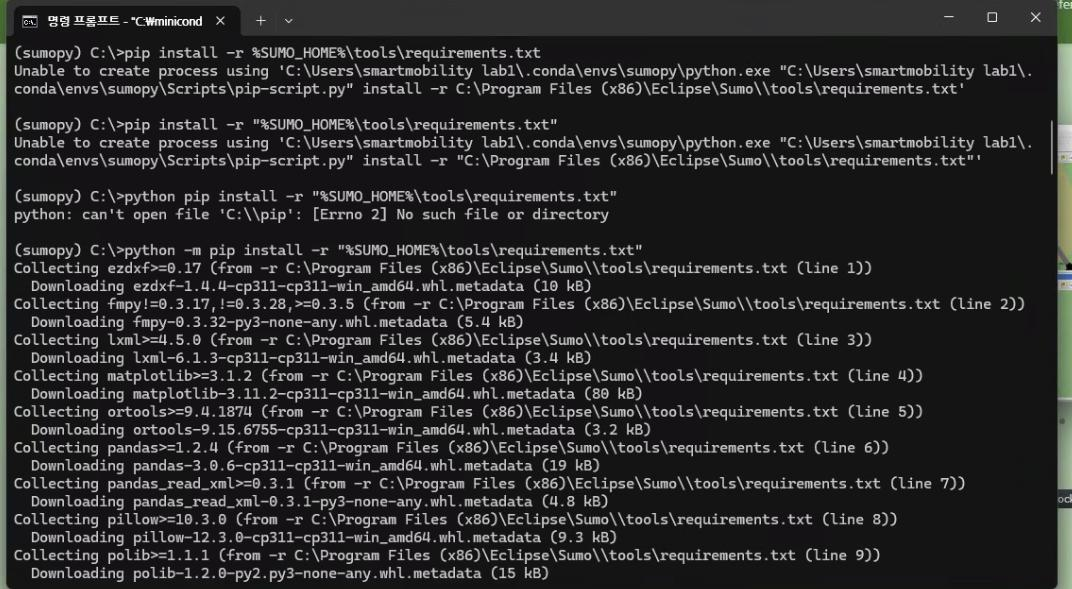
\includegraphics[keepaspectratio]{image/install_miniconda_6.jpeg}}

\begin{enumerate}
\def\labelenumi{\arabic{enumi}.}
\setcounter{enumi}{5}
\tightlist
\item
  sumopy를 활성화한 뒤에 sumo 관련 파이썬 코드를 사용하거나 관련
  패키지를 설치하는 것이 좋습니다.
\end{enumerate}

\chapter{SUMO 설치 : 윈도우}\label{sumo-uxc124uxce58-uxc708uxb3c4uxc6b0}

\begin{enumerate}
\def\labelenumi{\arabic{enumi}.}
\item
  \href{https://eclipse.dev/sumo/}{SUMO} 접속,
  \texttt{SUMO\ 1.27.1\ for\ Windows\ 64-bit}을 클릭하여 SUMO 설치
  프로그램 다운로드
  \pandocbounded{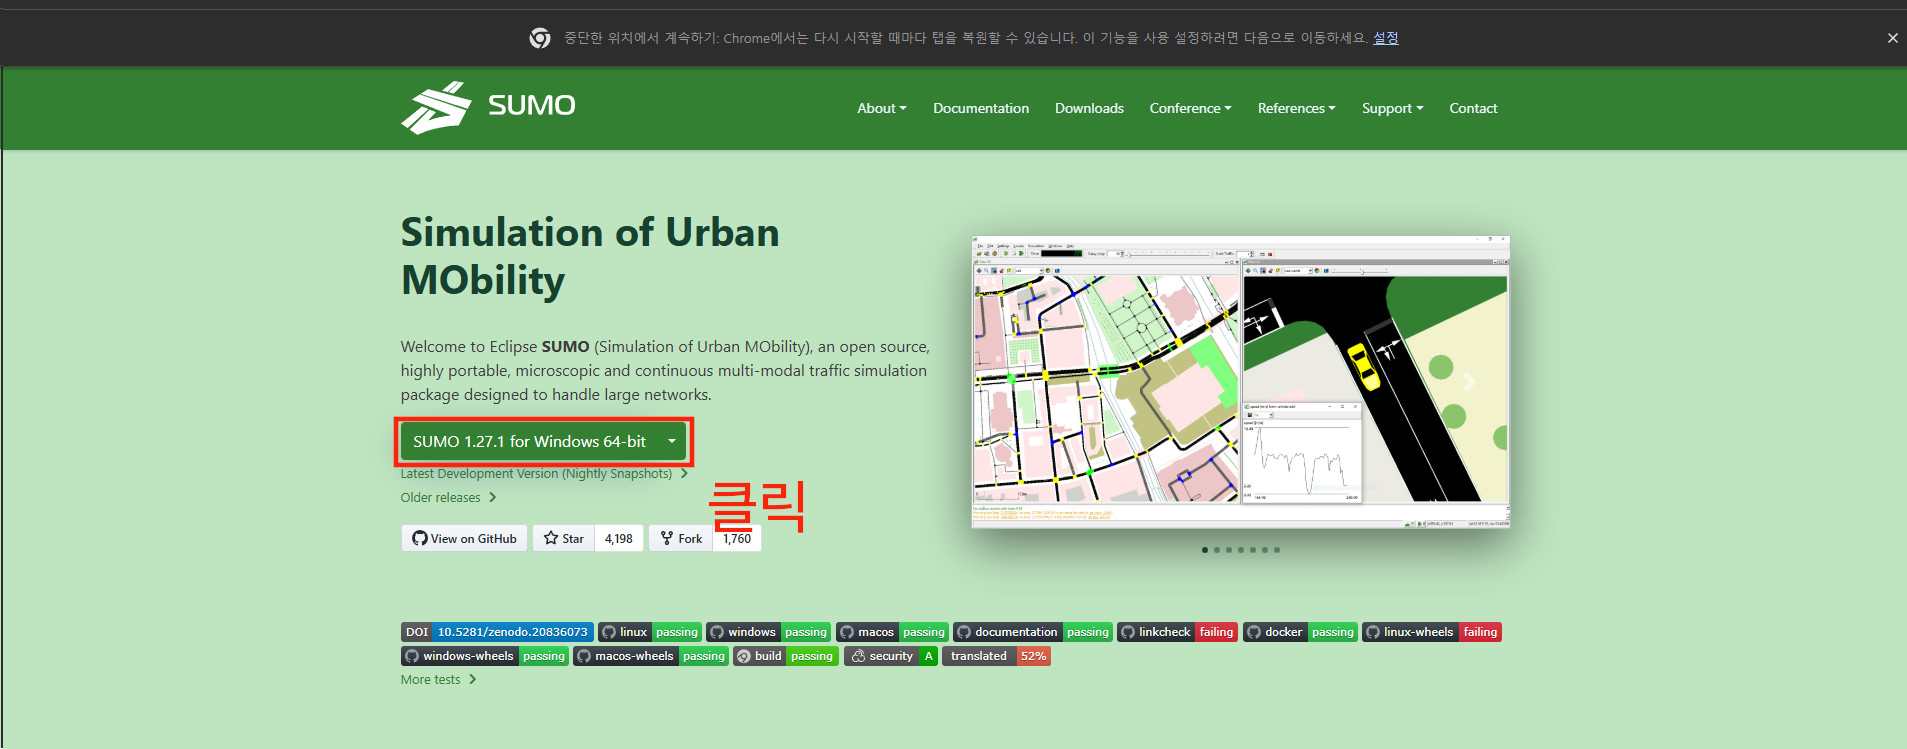
\includegraphics[keepaspectratio]{image/install_window_down1.jpeg}}
\item
  SUMO 설치 프로그램 클릭하여 설치 시작, SUMO 설치 주소는 디폴트 경로로
  유지, \texttt{set\ SUMO\_HOME\ and} 체크박스 선택
  \pandocbounded{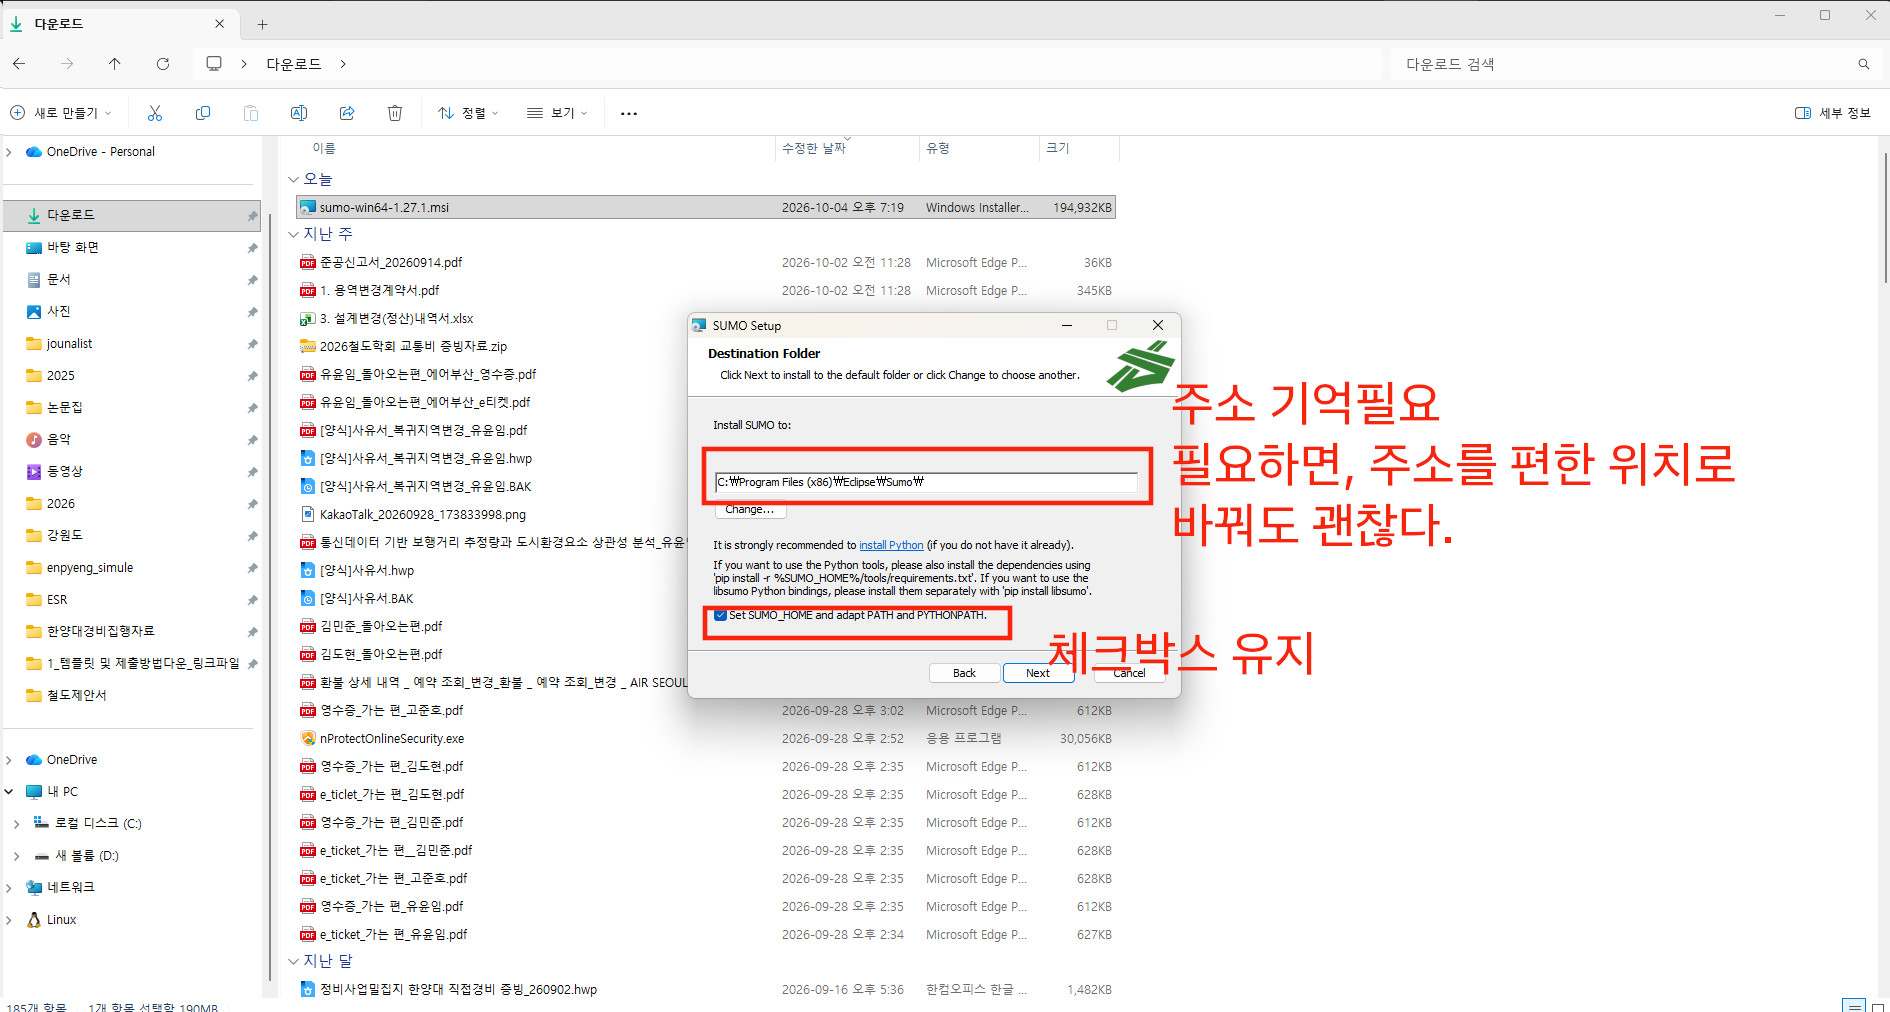
\includegraphics[keepaspectratio]{image/install_window_down3.jpeg}}
\item
  설정한 주소에 SUMO 폴더가 설치되어 있는지 확인

  \begin{itemize}
  \tightlist
  \item
    디폴트 경로대로 설치하였다면,
    \texttt{내\ pc\ \textgreater{}\ 로컬디스크\ C\ \textgreater{}\ Program\ Files\ (x86)\ \textgreater{}\ Eclipse\ \textgreater{}\ Sumo}에
    프로그램 폴더가 설치되어 있다.
    \pandocbounded{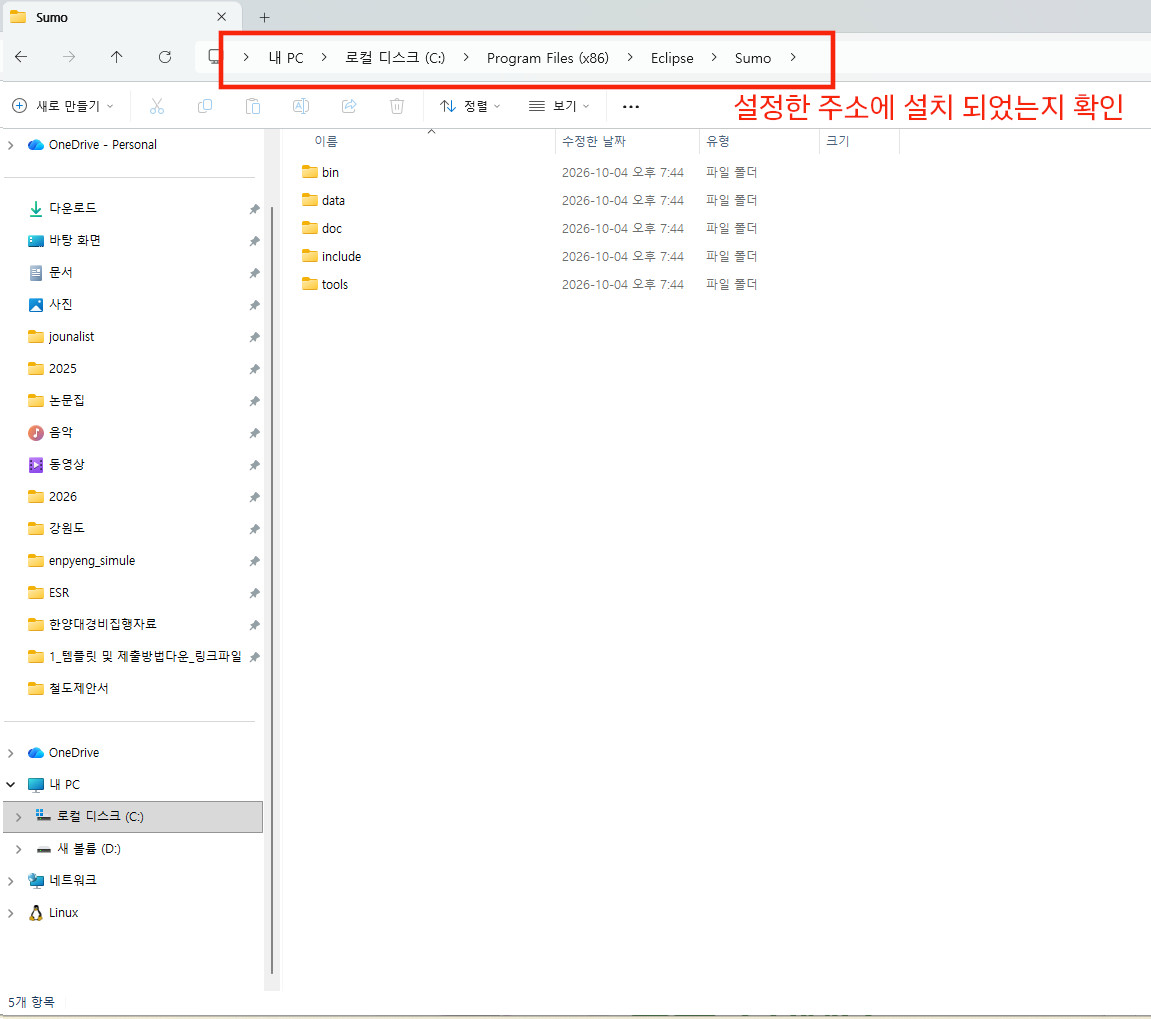
\includegraphics[keepaspectratio]{image/install_window_down4.jpeg}}
  \end{itemize}
\item
  tools 폴더 안에 SUMO python 프로그램이 있다. 각 프로그램별 기능은
  \href{https://sumo.dlr.de/docs/index.html}{SUMO document}에서 검색해서
  찾아볼 수 있다.
  \pandocbounded{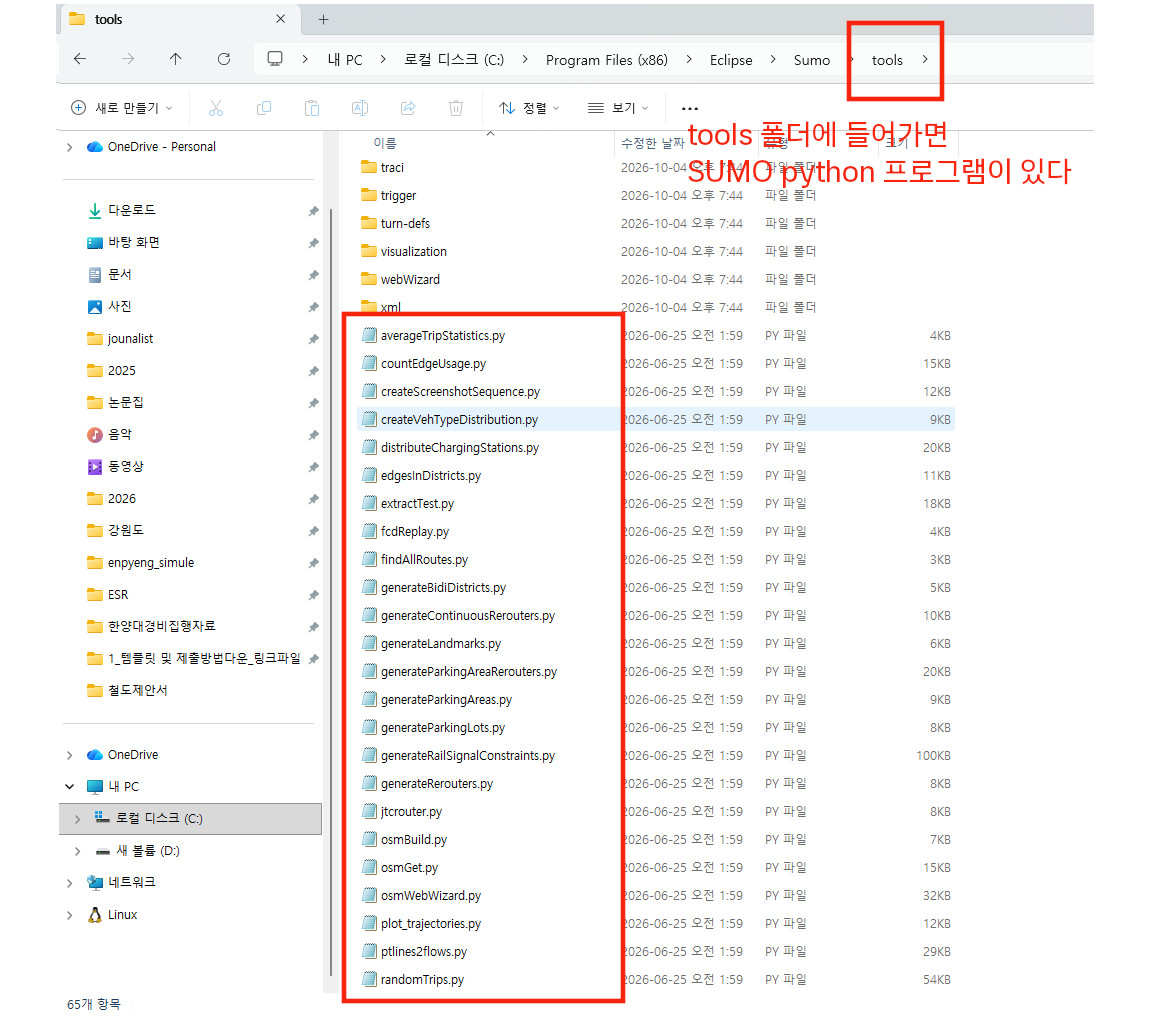
\includegraphics[keepaspectratio]{image/install_window_down5.jpeg}}
\item
  CMD 창을 켜서, SUMO가 잘 작동하는지 확인한다. 만약, 프로그램 폴더가
  있지만, CMD에서 sumo가 작동하지 않는다면 환경변수 설정에서 오류가 생긴
  것으로 아래 환경변수 설정을 따라하자.
\end{enumerate}

명령어 입력

\begin{Shaded}
\begin{Highlighting}[]
\NormalTok{sumo {-}}\AttributeTok{{-}version}
\end{Highlighting}
\end{Shaded}

\pandocbounded{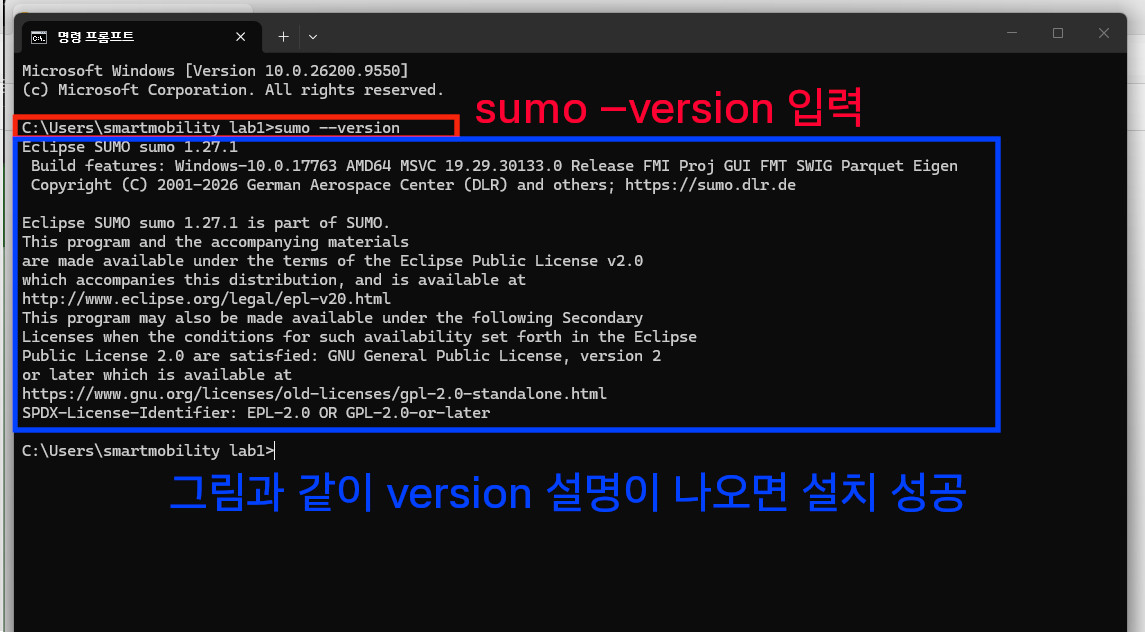
\includegraphics[keepaspectratio]{image/install_window_down7.jpeg}}

\section{sumo 환경변수
설정}\label{sumo-uxd658uxacbduxbcc0uxc218-uxc124uxc815}

환경변수 설정 1. sumo bin path를 환경변수로 설정해야합니다. 2. SUMO Path
환경변수 설정하기 3.내가 설치한 SUMO 폴더를 찾는다 4.SUMO 폴더에
들어간다 5.bin폴더에 들어간다. 6.폴더 바탕에서 오른쪽 키를 클릭한다
7.속성을 클릭한다 8.보안탭에 들어간다 9.개체 이름을 복사한다. 10. 복사한
값은 sumo bin 폴더의 path(주소)이다. 11.
\texttt{F:\textbackslash{}Program\ Files\textbackslash{}sumo\textbackslash{}bin}(자기
sumo\textgreater bin 폴더의 주소값) 12.
윈도우키\textgreater 설정\textgreater 시스템\textgreater 정보\textgreater 고급시스템
설정 \textgreater 고급 Tab clik 1. 환경변수 클릭 2. Path 클릭 3. 편집
클릭 4. 새로만들기 클릭 5. 복사한 주소값 넣기 6. 적용 7. cmd 켜기 8.
작동확인 9. ppt에 나와있는대로 SUMO\_HOME, Path에 sumo bin 구성되어 있는
지 확인 10. 안되면 sumo 삭제 후, 디폴트 상태로 재설치(환경변수 추가에
Check하여 설치) or 메일로 문의

\pandocbounded{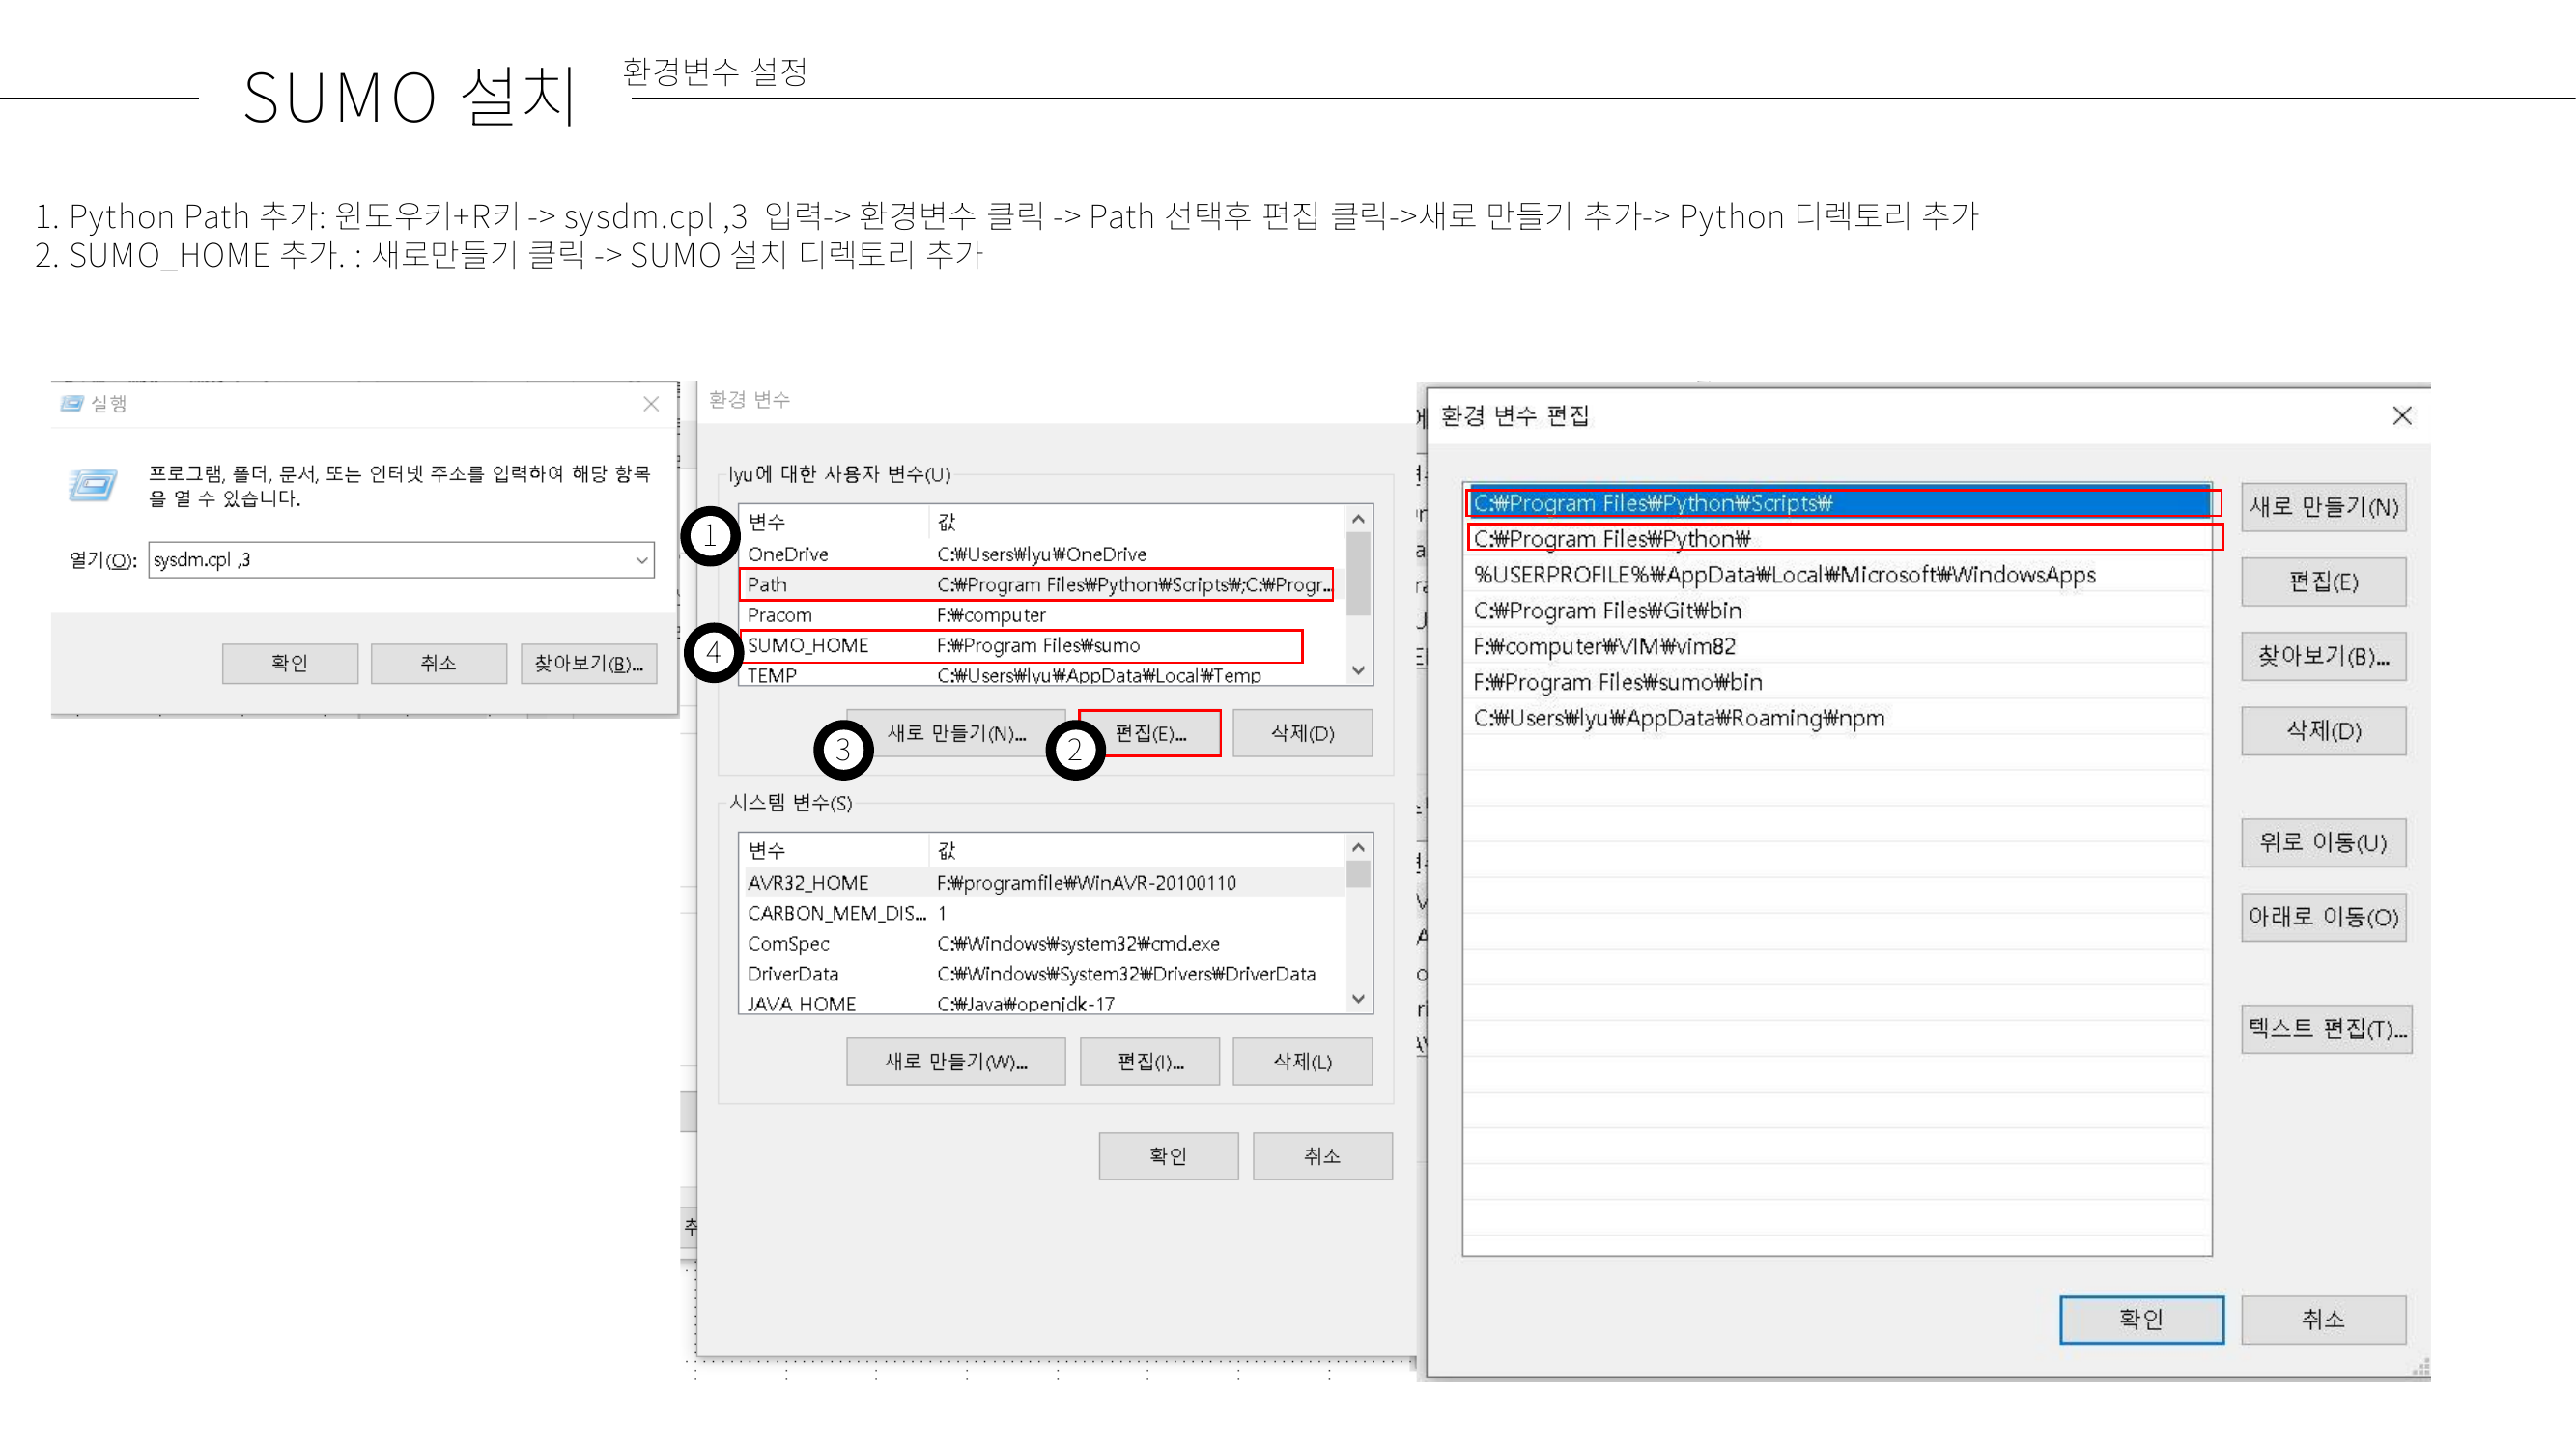
\includegraphics[keepaspectratio]{image/page-09.png}}

\chapter{MAC 설치}\label{mac-uxc124uxce58}

\href{https://sumo.dlr.de/docs/Installing/MacOS_Build.html}{sumo mac
build} https://sumo.dlr.de/docs/Downloads.php\#macos download sumo
SUMO\_HOME environment sumo lunchers download

\subsection{git 설치, Homebrew
설치}\label{git-uxc124uxce58-homebrew-uxc124uxce58}

아래 블로그 링크 따라하기

\href{https://velog.io/@wiseah/Git-\%EC\%84\%A4\%EC\%B9\%98-\%EB\%B0\%8F-\%ED\%99\%98\%EA\%B2\%BD\%EC\%84\%A4\%EC\%A0\%95mac-os}{wiseah
블로그}

\subsection{First}\label{first}

\begin{enumerate}
\def\labelenumi{\arabic{enumi}.}
\tightlist
\item
  Python 설치

  \begin{enumerate}
  \def\labelenumii{\arabic{enumii}.}
  \tightlist
  \item
    terminal
  \end{enumerate}

\begin{verbatim}
brew install python3       
\end{verbatim}
\end{enumerate}

\begin{Shaded}
\begin{Highlighting}[]
\ExtensionTok{python3} \AttributeTok{{-}V}
\end{Highlighting}
\end{Shaded}

\begin{Shaded}
\begin{Highlighting}[]
\FunctionTok{vi}\NormalTok{ \textasciitilde{}/.zshrc}
\end{Highlighting}
\end{Shaded}

\begin{Shaded}
\begin{Highlighting}[]
\NormalTok{alias python ="python3"}
\NormalTok{esc + : wq}
\end{Highlighting}
\end{Shaded}

\begin{Shaded}
\begin{Highlighting}[]
\BuiltInTok{source}\NormalTok{ \textasciitilde{}/.zshrc}
\end{Highlighting}
\end{Shaded}

https://priming.tistory.com/154 https://jerryjerryjerry.tistory.com/90

\begin{enumerate}
\def\labelenumi{\arabic{enumi}.}
\setcounter{enumi}{1}
\tightlist
\item
  XQuartz 설치

  \begin{enumerate}
  \def\labelenumii{\arabic{enumii}.}
  \tightlist
  \item
    \href{https://www.xquartz.org/}{https://www.xquartz.org} 접속
  \item
    .dmg 파일 다운로드
  \item
    shift+우클릭 다운로드 파일 진행
  \item
    mac 로그아웃, 로그인
  \item
    Launchpad\textgreater{} 기타
  \item
    \$ ssh -X root@local IP sumo
  \end{enumerate}
\end{enumerate}

참고 : https://blog.naver.com/asa4209/222219869485 3. sumo-1.24.0.pkg
설치

\section{second}\label{second}

\subsection{Hombrew install is
recommended}\label{hombrew-install-is-recommended}

\begin{itemize}
\tightlist
\item
  terminal 켜기
  \pandocbounded{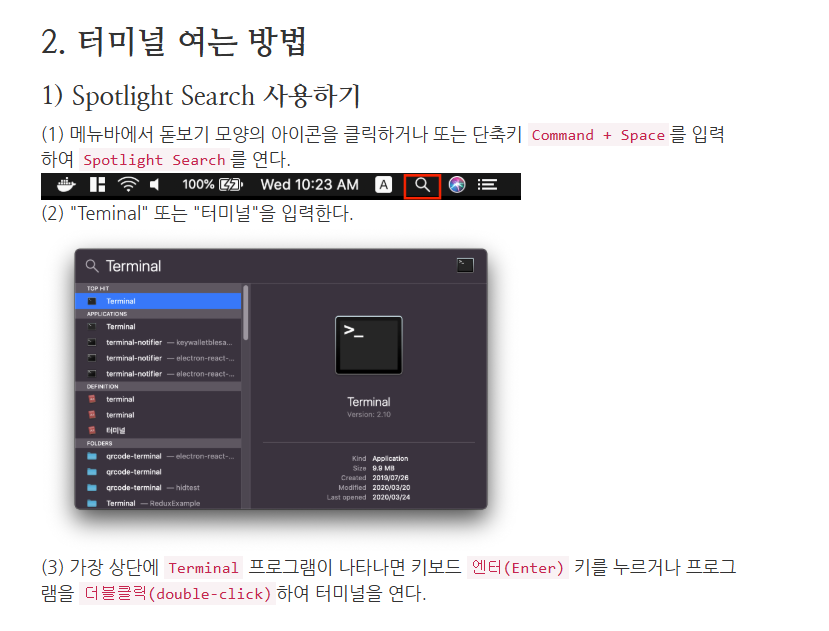
\includegraphics[keepaspectratio]{image/Pasted image 20251103204710.png}}
\end{itemize}

termainal 순서대로 입력(복붙)

\begin{Shaded}
\begin{Highlighting}[]
\ExtensionTok{/bin/bash} \AttributeTok{{-}c} \StringTok{"}\VariableTok{$(}\ExtensionTok{curl} \AttributeTok{{-}fsSL}\NormalTok{ https://raw.githubusercontent.com/Homebrew/install/master/install.sh}\VariableTok{)}\StringTok{"}
\end{Highlighting}
\end{Shaded}

\begin{Shaded}
\begin{Highlighting}[]
\ExtensionTok{brew}\NormalTok{ update}
\end{Highlighting}
\end{Shaded}

\begin{Shaded}
\begin{Highlighting}[]
\ExtensionTok{xcode{-}select} \AttributeTok{{-}{-}install}
\end{Highlighting}
\end{Shaded}

\begin{Shaded}
\begin{Highlighting}[]
\FunctionTok{clang} \AttributeTok{{-}{-}version}
\end{Highlighting}
\end{Shaded}

\begin{Shaded}
\begin{Highlighting}[]
\ExtensionTok{brew}\NormalTok{ install cmake}
\end{Highlighting}
\end{Shaded}

\begin{Shaded}
\begin{Highlighting}[]
\ExtensionTok{brew}\NormalTok{ install }\AttributeTok{{-}{-}cask}\NormalTok{ xquartz}
\end{Highlighting}
\end{Shaded}

\begin{Shaded}
\begin{Highlighting}[]
\ExtensionTok{brew}\NormalTok{ install xerces{-}c fox proj gdal gl2ps}
\end{Highlighting}
\end{Shaded}

\begin{Shaded}
\begin{Highlighting}[]
\NormalTok{brew install python ccache googletest fmt swig eigen apache{-}arrow pygobject3 gtk+3 adwaita{-}icon{-}theme python3 {-}m pip install texttest}
\end{Highlighting}
\end{Shaded}

\begin{Shaded}
\begin{Highlighting}[]
\FunctionTok{git}\NormalTok{ clone }\AttributeTok{{-}{-}recursive}\NormalTok{ https://github.com/eclipse{-}sumo/sumo }
\end{Highlighting}
\end{Shaded}

\begin{Shaded}
\begin{Highlighting}[]
\BuiltInTok{export} \VariableTok{SUMO\_HOME}\OperatorTok{=}\StringTok{"}\VariableTok{$PWD}\StringTok{/sumo"}
\end{Highlighting}
\end{Shaded}

\begin{Shaded}
\begin{Highlighting}[]
\BuiltInTok{cd} \VariableTok{$SUMO\_HOME}
\end{Highlighting}
\end{Shaded}

\begin{Shaded}
\begin{Highlighting}[]
\FunctionTok{cmake} \AttributeTok{{-}B}\NormalTok{ build .}
\end{Highlighting}
\end{Shaded}

\begin{Shaded}
\begin{Highlighting}[]
\BuiltInTok{cd} \VariableTok{$SUMO\_HOME}
\end{Highlighting}
\end{Shaded}

\begin{Shaded}
\begin{Highlighting}[]
\FunctionTok{cmake} \AttributeTok{{-}{-}build}\NormalTok{ build }\AttributeTok{{-}{-}parallel} \VariableTok{$(}\ExtensionTok{sysctl} \AttributeTok{{-}n}\NormalTok{ hw.ncpu}\VariableTok{)}
\end{Highlighting}
\end{Shaded}

Download SUMO lanchers

\part{SUMO 기초 실습}

간단한 네트워크 만들기와 통행 생성을 통해서 SUMO 시뮬레이션을 해보는
장입니다. 간단한 실습을 통해서 SUMO를 사용해보는 것이 목적입니다. 이
실습 장 이후에 SUMO 이론과 동작 순서를 설명하겠습니다. 이런 프로그램은
우선 일단 한 번 돌려보면, 사용 순서나 프로그램이 구현하고자 하는 개념을
쉽게 이해할 수 있는 것 같습니다.

실습을 하기 이전에 프로젝트 폴더 만들기, Net Edit 프로그램 여는 법, Net
Edit에서 네트워크 저장하는 법, VS CODE에서 프로젝트 폴더 여는 법, VS
CODE에서 CMD 여는 법을 먼저 설명 드리겠습니다.

\section*{프로젝트 폴더
생성}\label{uxd504uxb85cuxc81duxd2b8-uxd3f4uxb354-uxc0dduxc131}
\addcontentsline{toc}{section}{프로젝트 폴더 생성}

\markright{프로젝트 폴더 생성}

SUMO 시뮬레이션을 위해서는 많은 입력 파일이 필요합니다. 한 개의 폴더에서
시뮬레이션 입력 파일을 관리하는 것이 오류를 찾고, 고치기에 더 쉽습니다.
그래서 하나의 시뮬레이션에 하나의 폴더를 만드는 것이 좋습니다.

폴더 경로명에 한글이 있으면 오류가 생길 수 있습니다. 영문으로 된 경로에
시뮬레이션 프로젝트를 생성하는 것이 좋습니다.
\texttt{D:\textbackslash{}2026\textbackslash{}2026\_sumo\_tutorial\textbackslash{}basic\_example}과
같은 경로를 권장합니다.
\pandocbounded{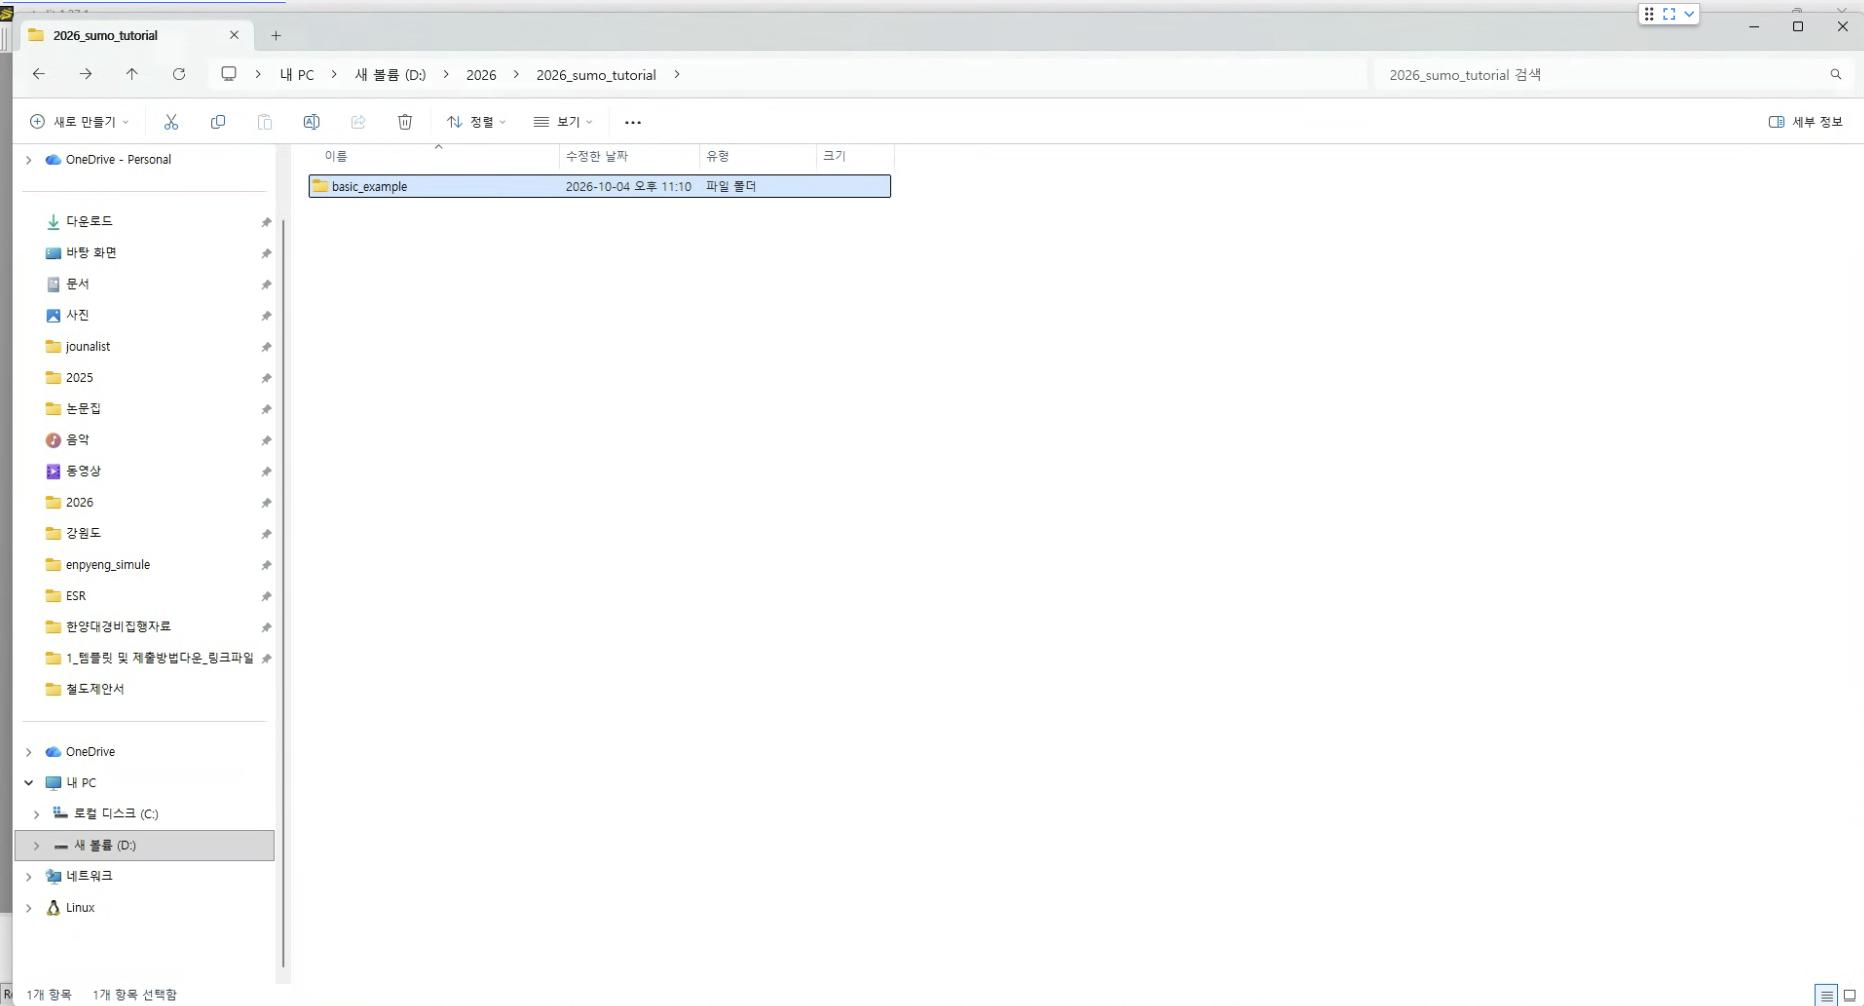
\includegraphics[keepaspectratio]{image/basic_1.jpeg}}

\section*{Net Edit}\label{net-edit}
\addcontentsline{toc}{section}{Net Edit}

\markright{Net Edit}

Net Edit은 SUMO 네트워크를 생성, 편집할 수 있는 GUI 프로그램입니다.
SUMO를 설치한 후, 윈도우 프로그램 창에 \texttt{Net\ Edit}을 검색하여
프로그램을 찾고, 열 수 있습니다.
\texttt{ctrl+s\textquotesingle{}\ 혹은}File\textgreater{} Save
Network`로 네트워크를 저장할 수 있습니다.

\pandocbounded{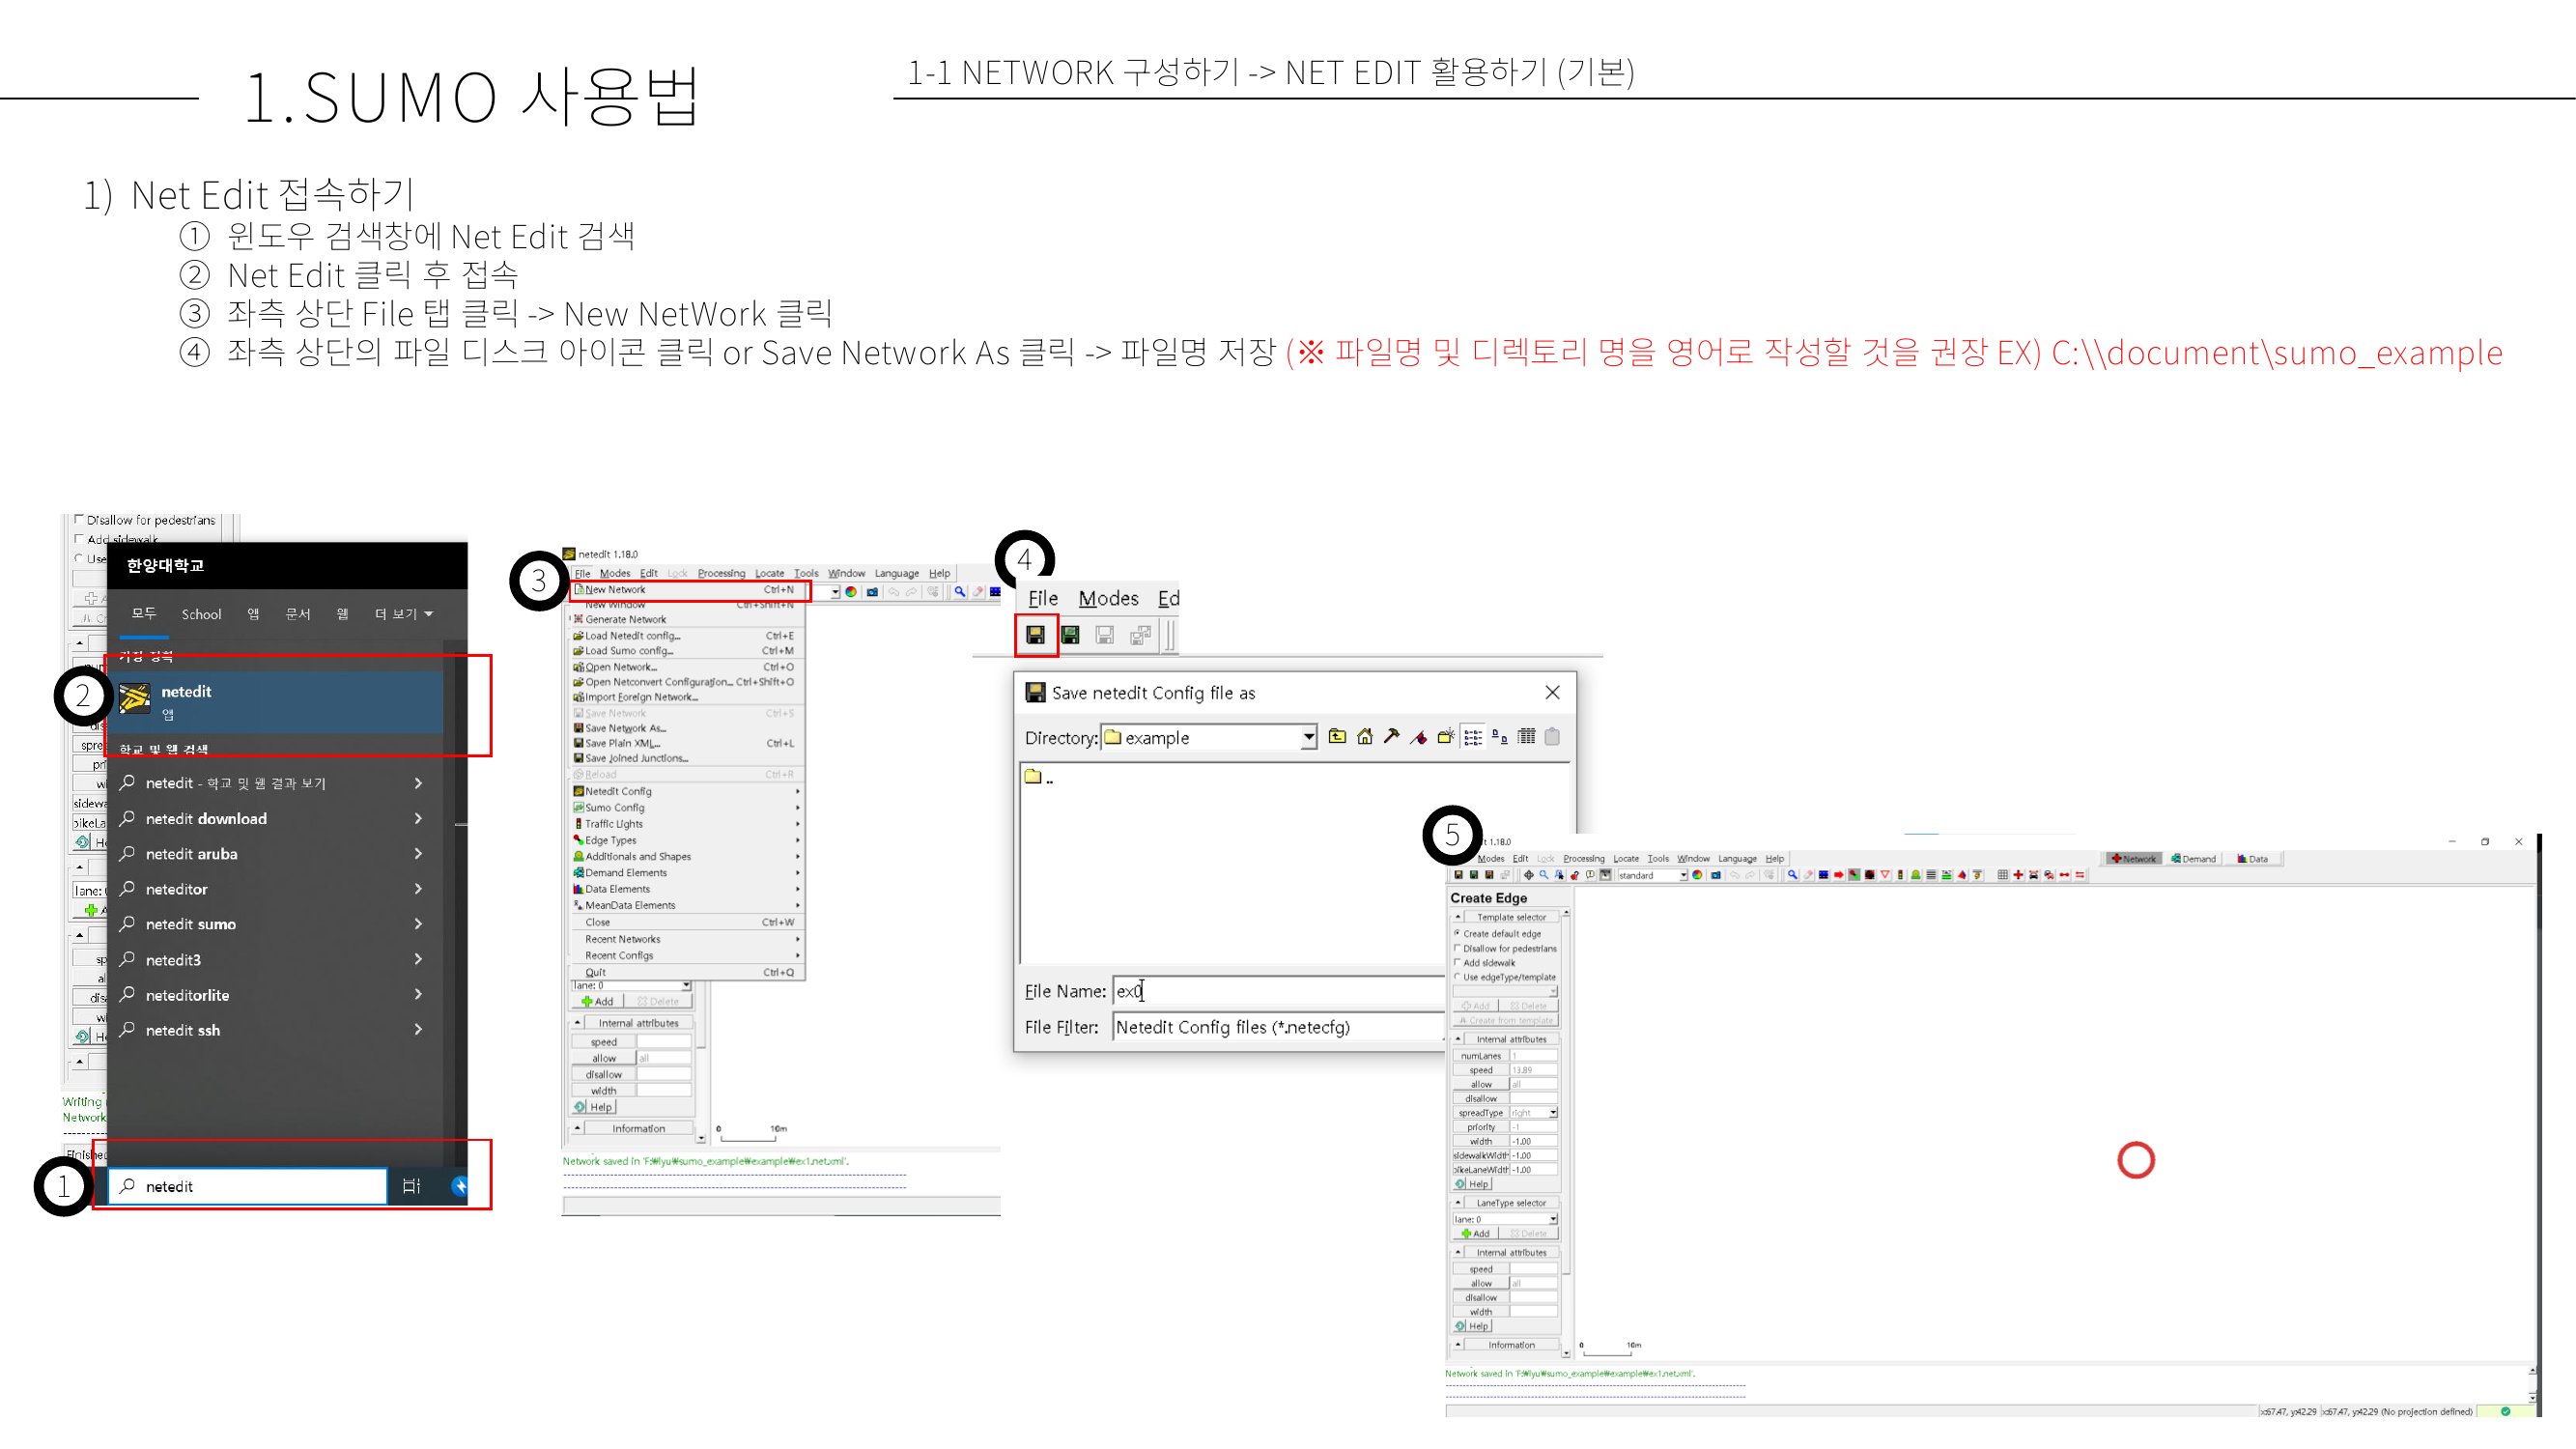
\includegraphics[keepaspectratio]{image/page-14.png}}

\subsection*{Net edit 기초
도구}\label{net-edit-uxae30uxcd08-uxb3c4uxad6c}
\addcontentsline{toc}{subsection}{Net edit 기초 도구}

Network를 작성하는 가장 기초적인 도구입니다. 그 외 도구 설명은
\href{https://sumo.dlr.de/docs/Netedit/index.html}{SUMO Documentation -
Net Edit} 참고 바랍니다.

\begin{enumerate}
\def\labelenumi{\arabic{enumi}.}
\tightlist
\item
  Inspect tool

  \begin{itemize}
  \tightlist
  \item
    오브젝트 정보 보기 \& 수정

    \begin{itemize}
    \tightlist
    \item
      ID 수정
    \item
      Node - Edge 연결정보 수정
    \item
      개체 속성값(최고 속도, 수단) 수정 등\\
    \end{itemize}
  \end{itemize}
\item
  Delete tool

  \begin{itemize}
  \tightlist
  \item
    오브젝트 삭제
  \end{itemize}
\item
  Drawing tool

  \begin{itemize}
  \tightlist
  \item
    Edge 생성
  \end{itemize}
\item
  Connection Tool

  \begin{itemize}
  \tightlist
  \item
    좌우회전, 유턴 등 Edge의 차선 lane 간의 교차로 연결 정보 보기 및
    수정 기능
  \end{itemize}
\item
  Traffic Light tool

  \begin{itemize}
  \tightlist
  \item
    교차로(Node)에 신호 정보 생성
  \item
    신호 현시 설정
  \item
    신호 간 offset 설정
  \end{itemize}
\item
  Hide junction

  \begin{itemize}
  \tightlist
  \item
    Juntion(Node) 도형 숨기기, 표출하기
  \item
    Edg와 Node 간 연결이 이상할 때, 해당 기능을 이용하여 lane 간 연결을
    볼 수 있다.
  \end{itemize}
\item
  Edge Opposite Direction

  \begin{itemize}
  \tightlist
  \item
    쌍방향 Edge를 한 번에 그릴 수 있다.
  \end{itemize}
\end{enumerate}

\pandocbounded{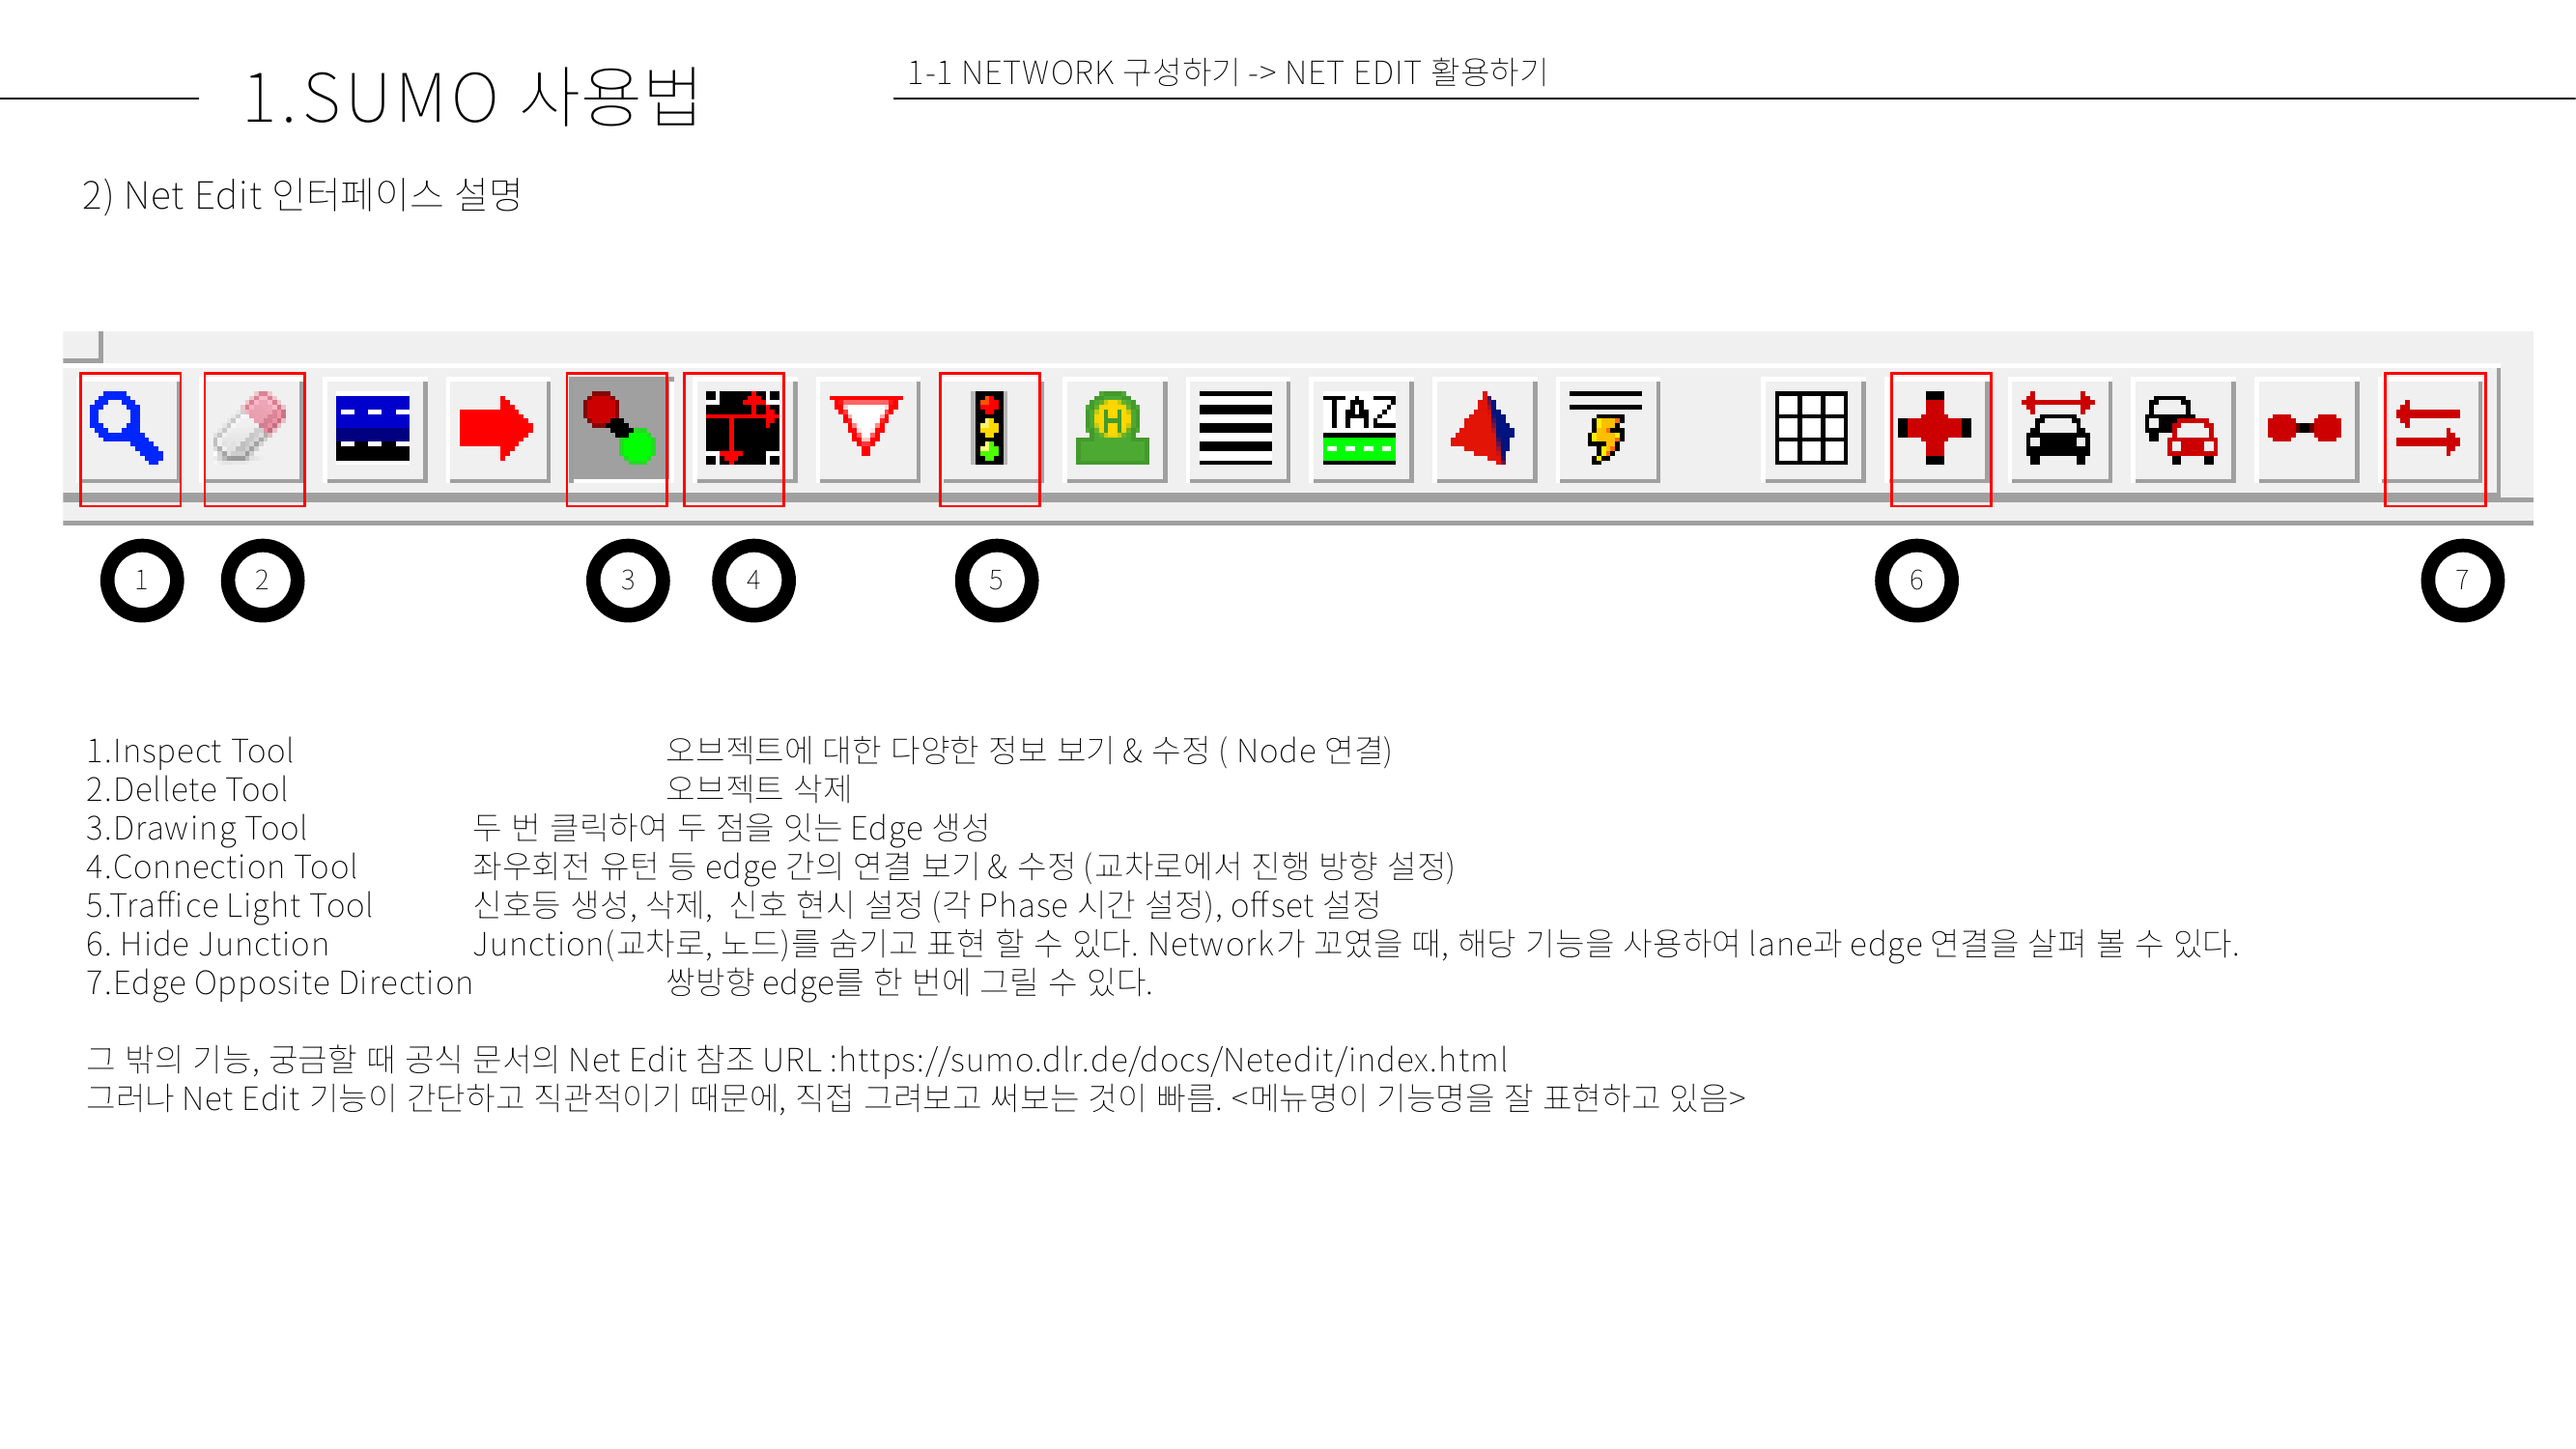
\includegraphics[keepaspectratio]{image/page-15.png}}

Inspect tool 패널에서 볼 수 있는 Edge 속성 설명

\pandocbounded{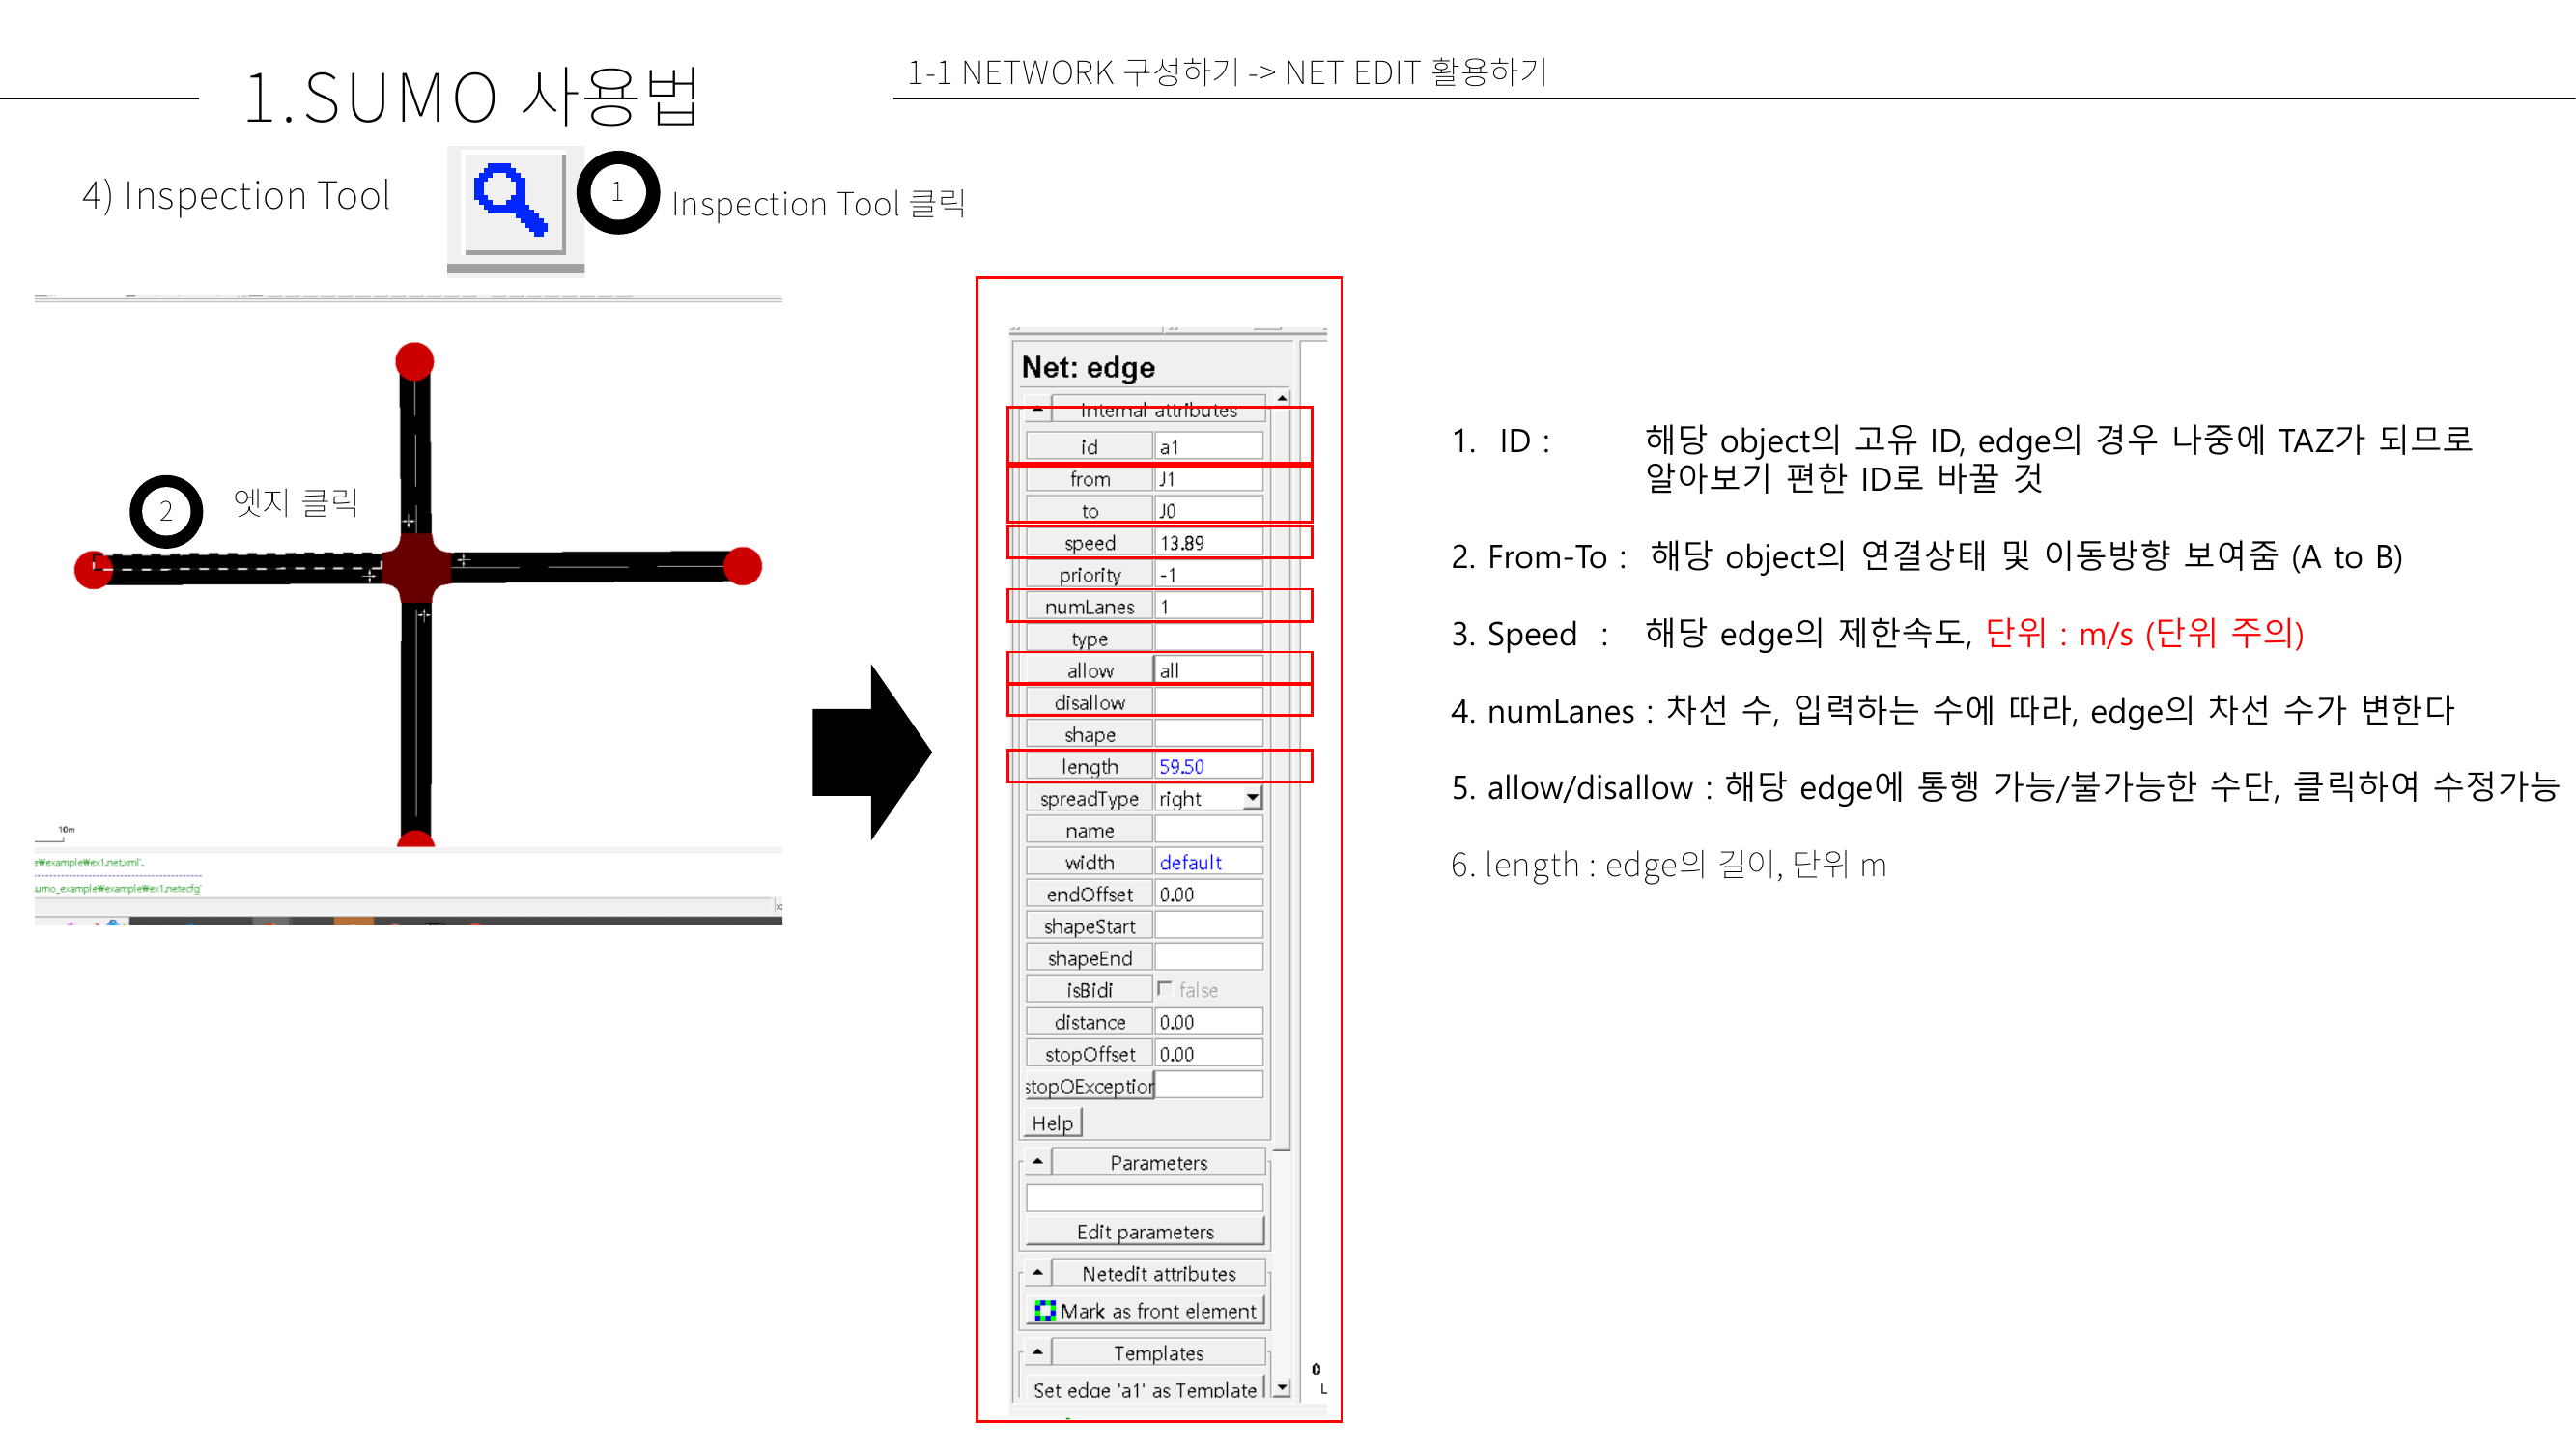
\includegraphics[keepaspectratio]{image/page-17.png}}

\section*{VS CODE}\label{vs-code}
\addcontentsline{toc}{section}{VS CODE}

\markright{VS CODE}

\subsection*{VS CODE에서 프로젝트 폴더 여는
법}\label{vs-codeuxc5d0uxc11c-uxd504uxb85cuxc81duxd2b8-uxd3f4uxb354-uxc5ecuxb294-uxbc95}
\addcontentsline{toc}{subsection}{VS CODE에서 프로젝트 폴더 여는 법}

\begin{enumerate}
\def\labelenumi{\arabic{enumi}.}
\item
  윈도우 프로그램 창에서 \texttt{vs\ code} 검색해서 vs code 열기
\item
  \texttt{File\textgreater{}\ Open\ Foler} 클릭
  \pandocbounded{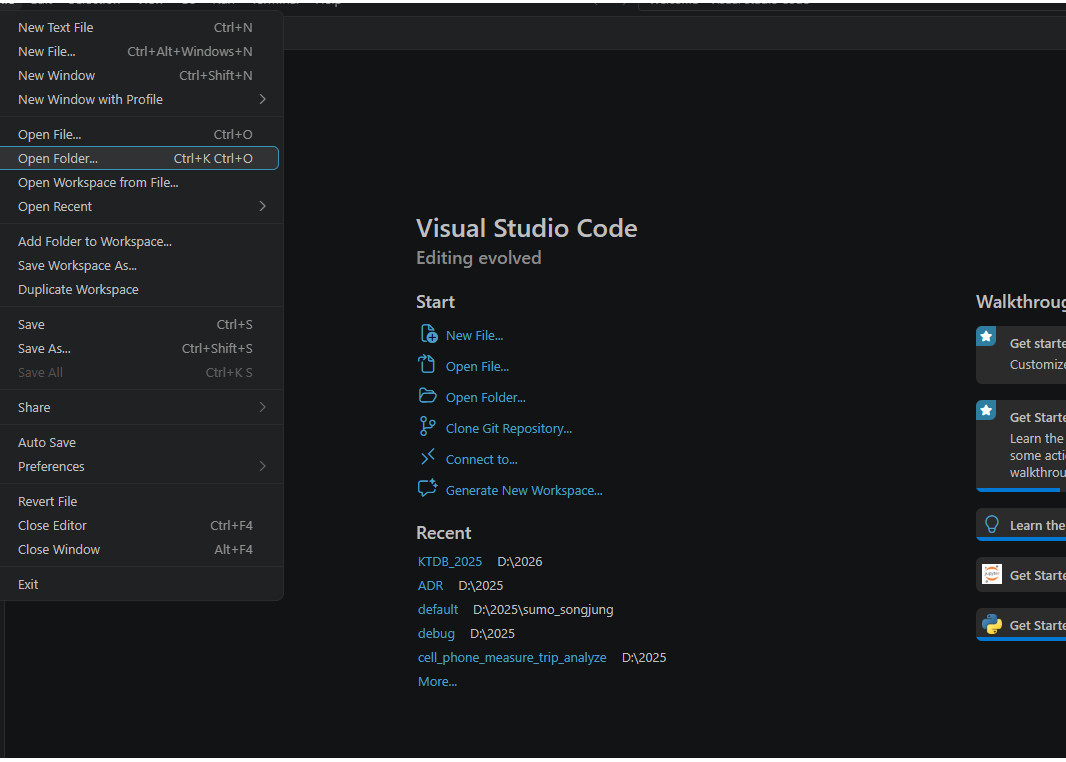
\includegraphics[keepaspectratio]{image/basic_prev0.jpeg}}
\item
  미리 생성하여 둔 프로젝트 경로 폴더 선택.
  \texttt{D:\textbackslash{}2026\textbackslash{}2026\_sumo\_tutorial\textbackslash{}basic\_example}
  \pandocbounded{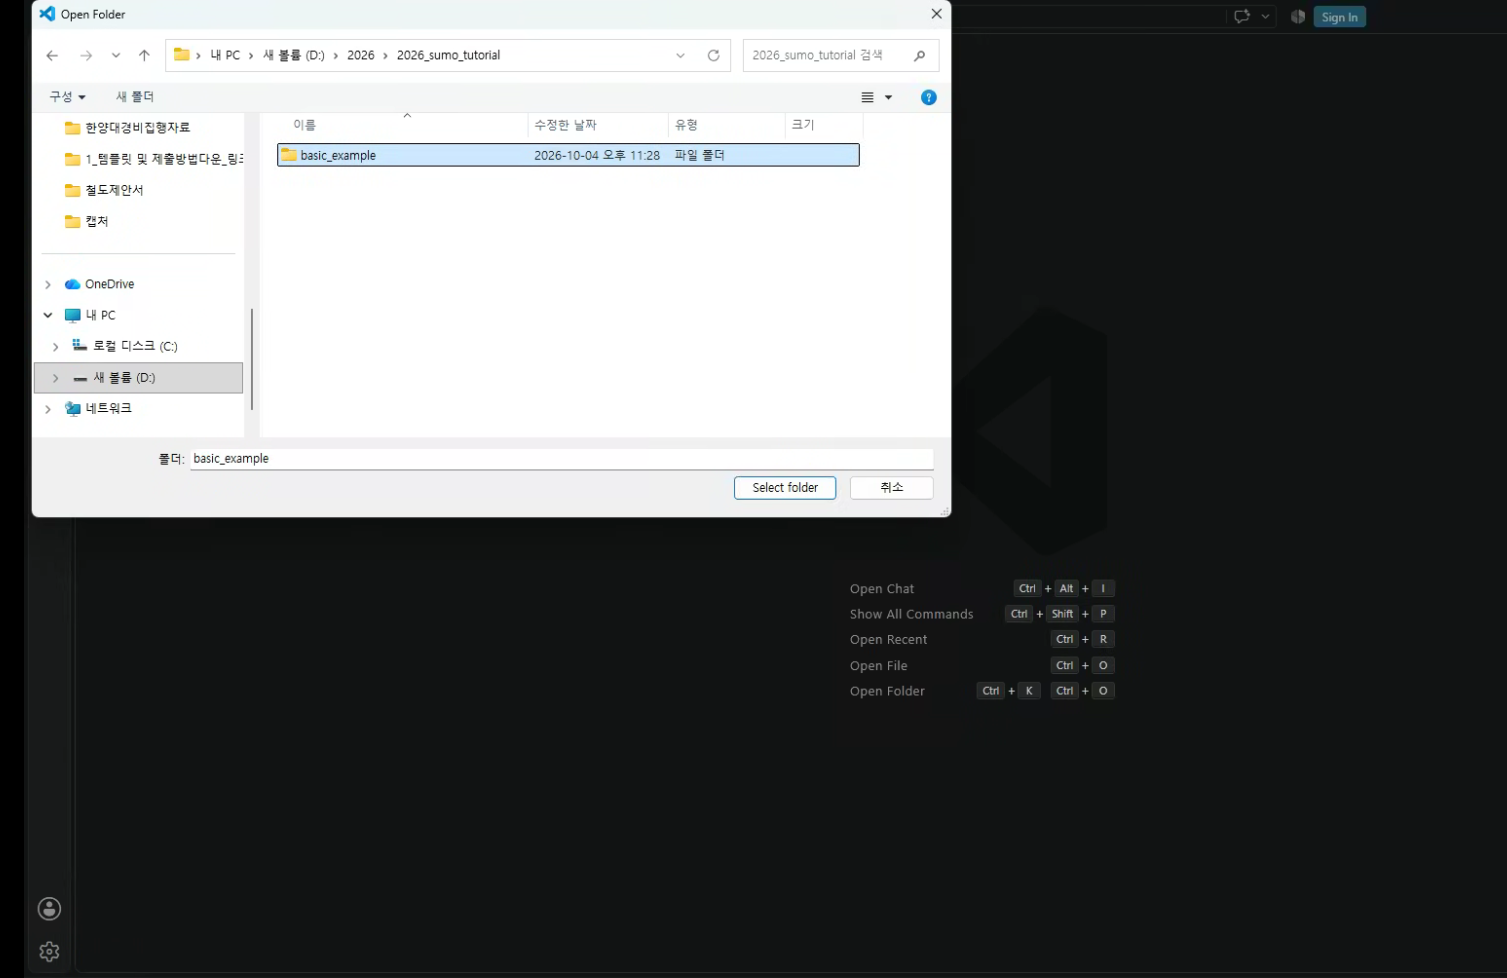
\includegraphics[keepaspectratio]{image/basic_prev01.png}}
\end{enumerate}

\subsection*{VS CODE에서 CMD 여는
법}\label{vs-codeuxc5d0uxc11c-cmd-uxc5ecuxb294-uxbc95}
\addcontentsline{toc}{subsection}{VS CODE에서 CMD 여는 법}

\begin{enumerate}
\def\labelenumi{\arabic{enumi}.}
\tightlist
\item
  단축키 \texttt{ctrl\ +\ \textasciigrave{}} 누르기 or
  \texttt{Terminal\ \textgreater{}\ New\ Terminal} 클릭
\item
  하단 Tabl에서 Termianl tab을 고르고, + 버튼을 누르고 Command Prompt
  선택
  \pandocbounded{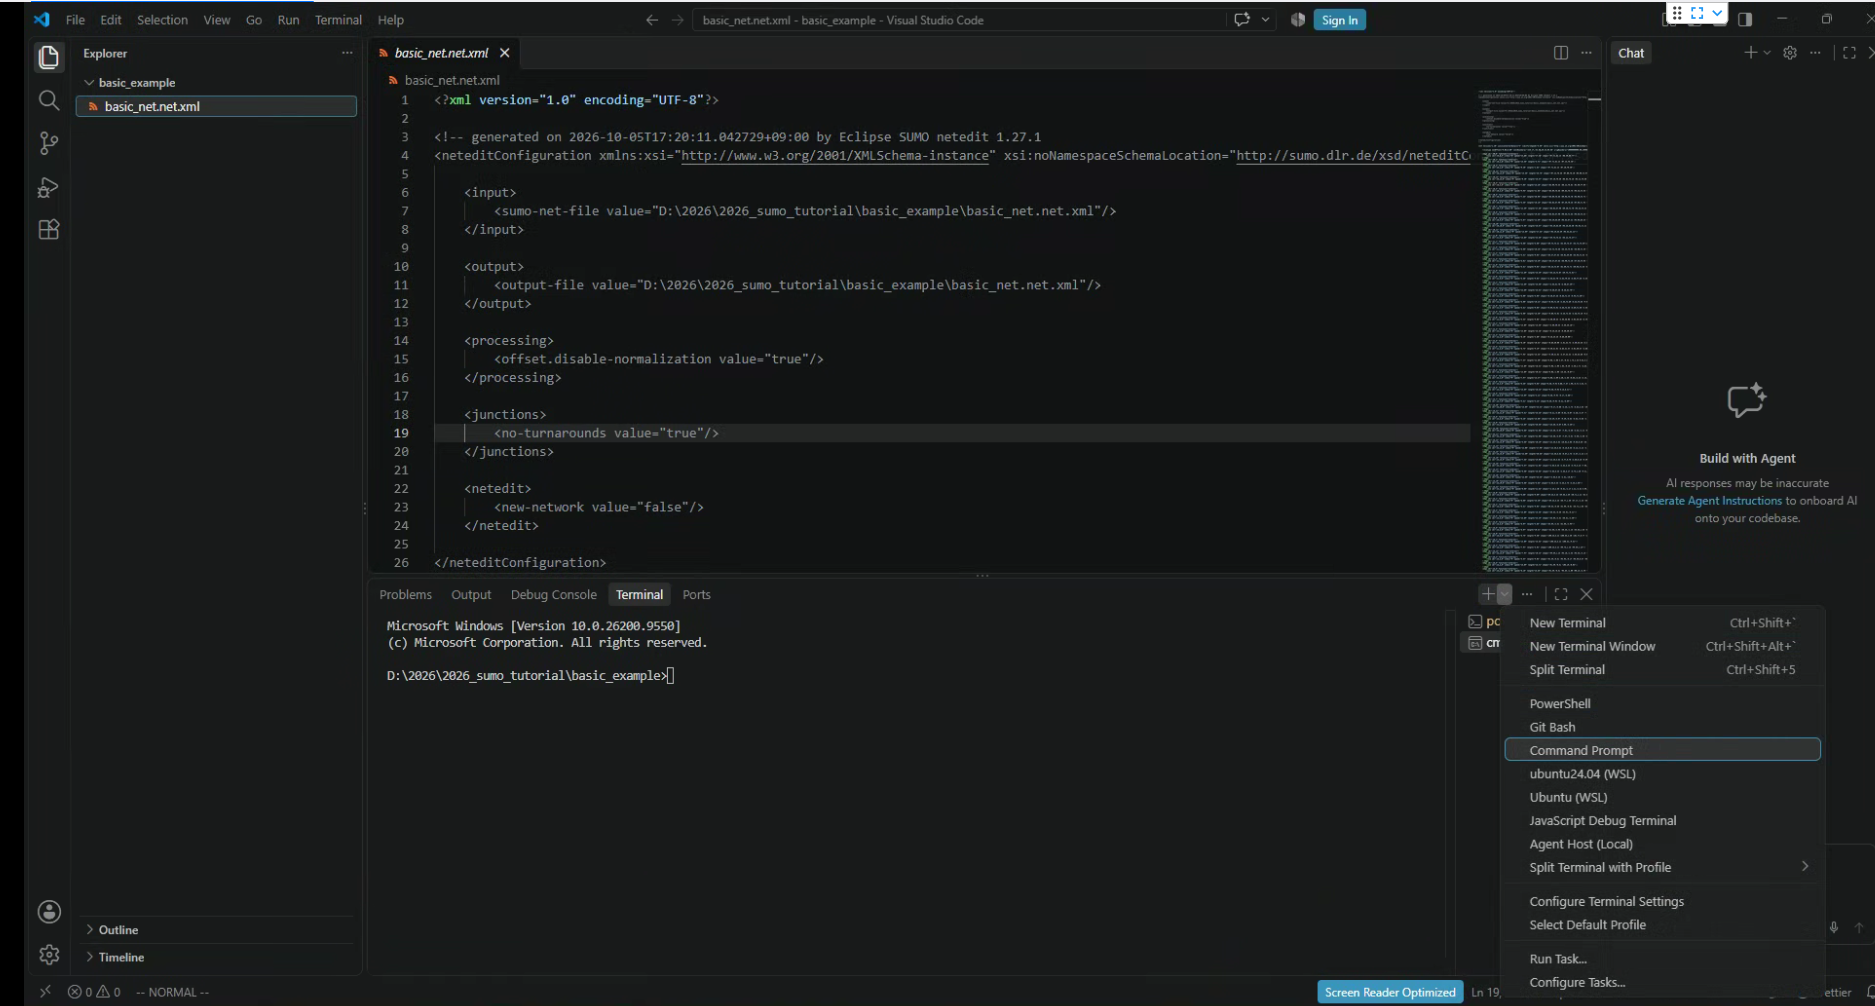
\includegraphics[keepaspectratio]{image/basic_prev02.png}}
\end{enumerate}

\chapter{Network 그리기}\label{network-uxadf8uxb9acuxae30}

\begin{enumerate}
\def\labelenumi{\arabic{enumi}.}
\tightlist
\item
  window 프로그램 창 열고, \texttt{net\ edit} 입력하여, network 편집기
  켜기

  \begin{itemize}
  \tightlist
  \item
    File \textgreater{} New Network 클릭
  \item
    File \textgreater{} Save Network As 클릭
  \item
    프로젝트 폴더 선택
  \item
    파일명으로 \texttt{basic\_net} 입력
  \end{itemize}
\item
  Edge Mode 클릭, Edge Opposite Direcition 클릭해서 아래 그림과 같이
  그리기

  \begin{itemize}
  \item
    완성 그림
    \pandocbounded{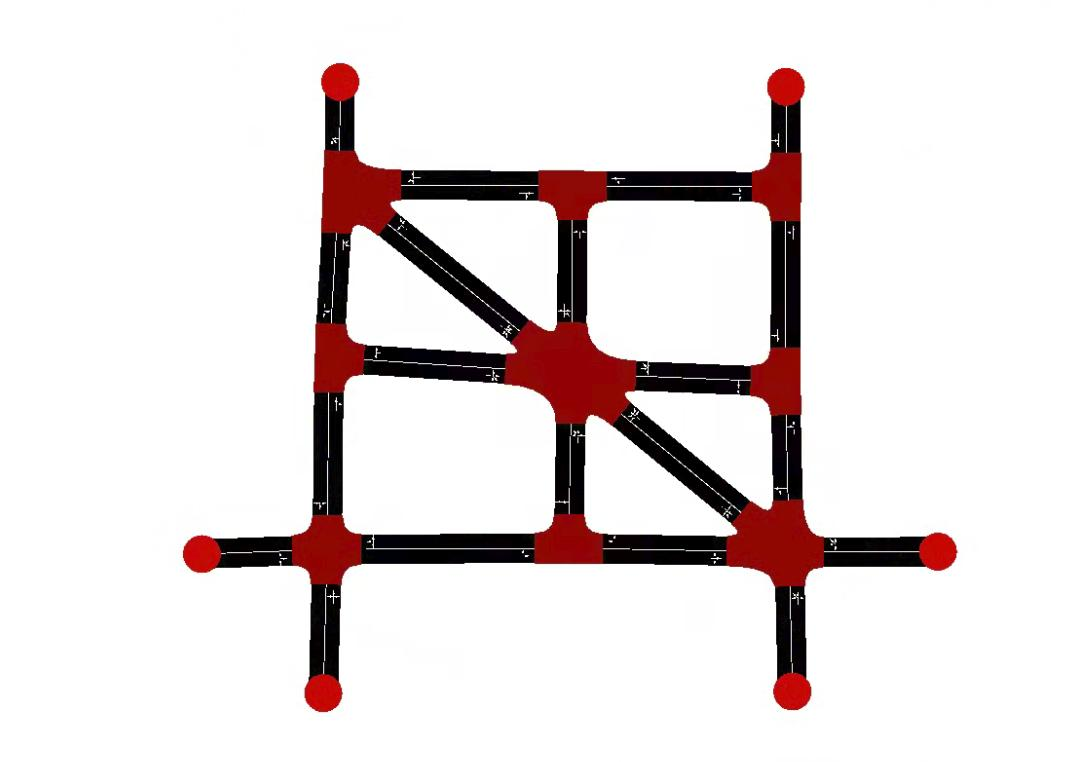
\includegraphics[keepaspectratio]{image/basic_2.jpeg}}
  \item
    EDGE 그리는 법 영상
  \end{itemize}
\end{enumerate}

\pandocbounded{\includegraphics[keepaspectratio]{image/ng.gif}}

\begin{enumerate}
\def\labelenumi{\arabic{enumi}.}
\setcounter{enumi}{2}
\tightlist
\item
  Inspect Tool 이용하여, 각 EDGE의 ID를 그림과 같이 입력해줍니다.

  \begin{itemize}
  \item
    목표 그림
    \pandocbounded{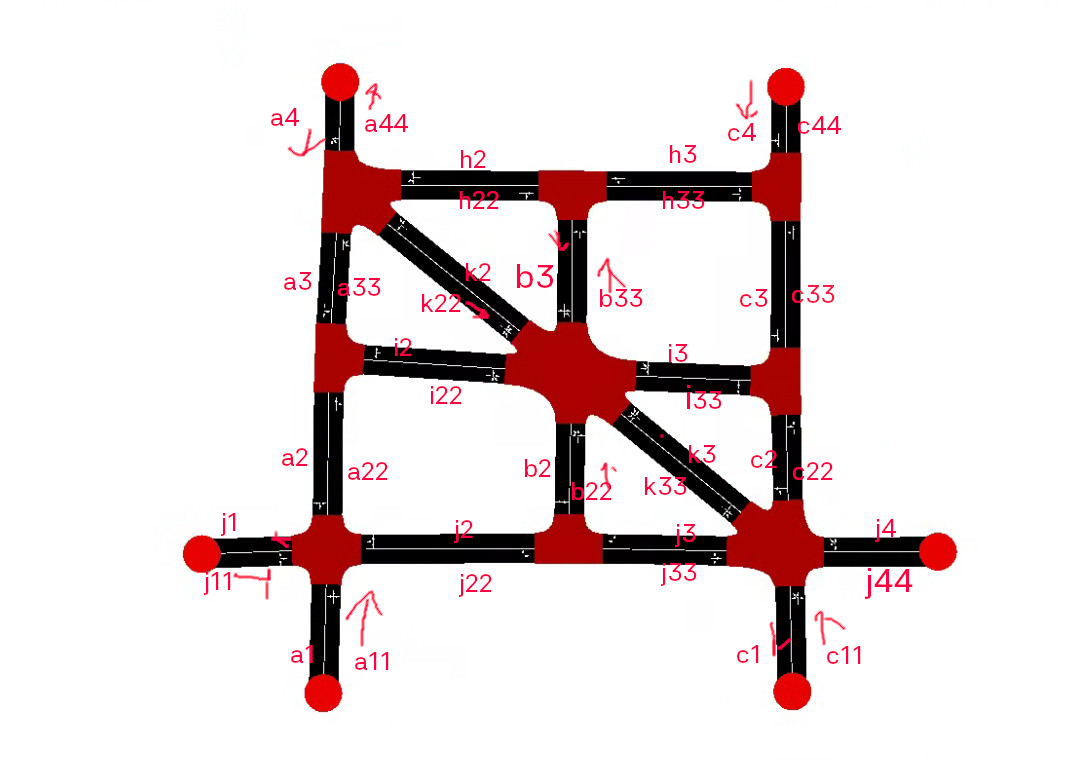
\includegraphics[keepaspectratio]{image/basic_3.jpeg}}
  \item
    ID 입력하는 법 영상
    \pandocbounded{\includegraphics[keepaspectratio]{image/id.gif}}
  \end{itemize}
\item
  VS CODE에서 프로젝트 폴더를 열면, \texttt{basic\_net.net.xml}이 생성된
  것을 확인할 수 있습니다.
  \pandocbounded{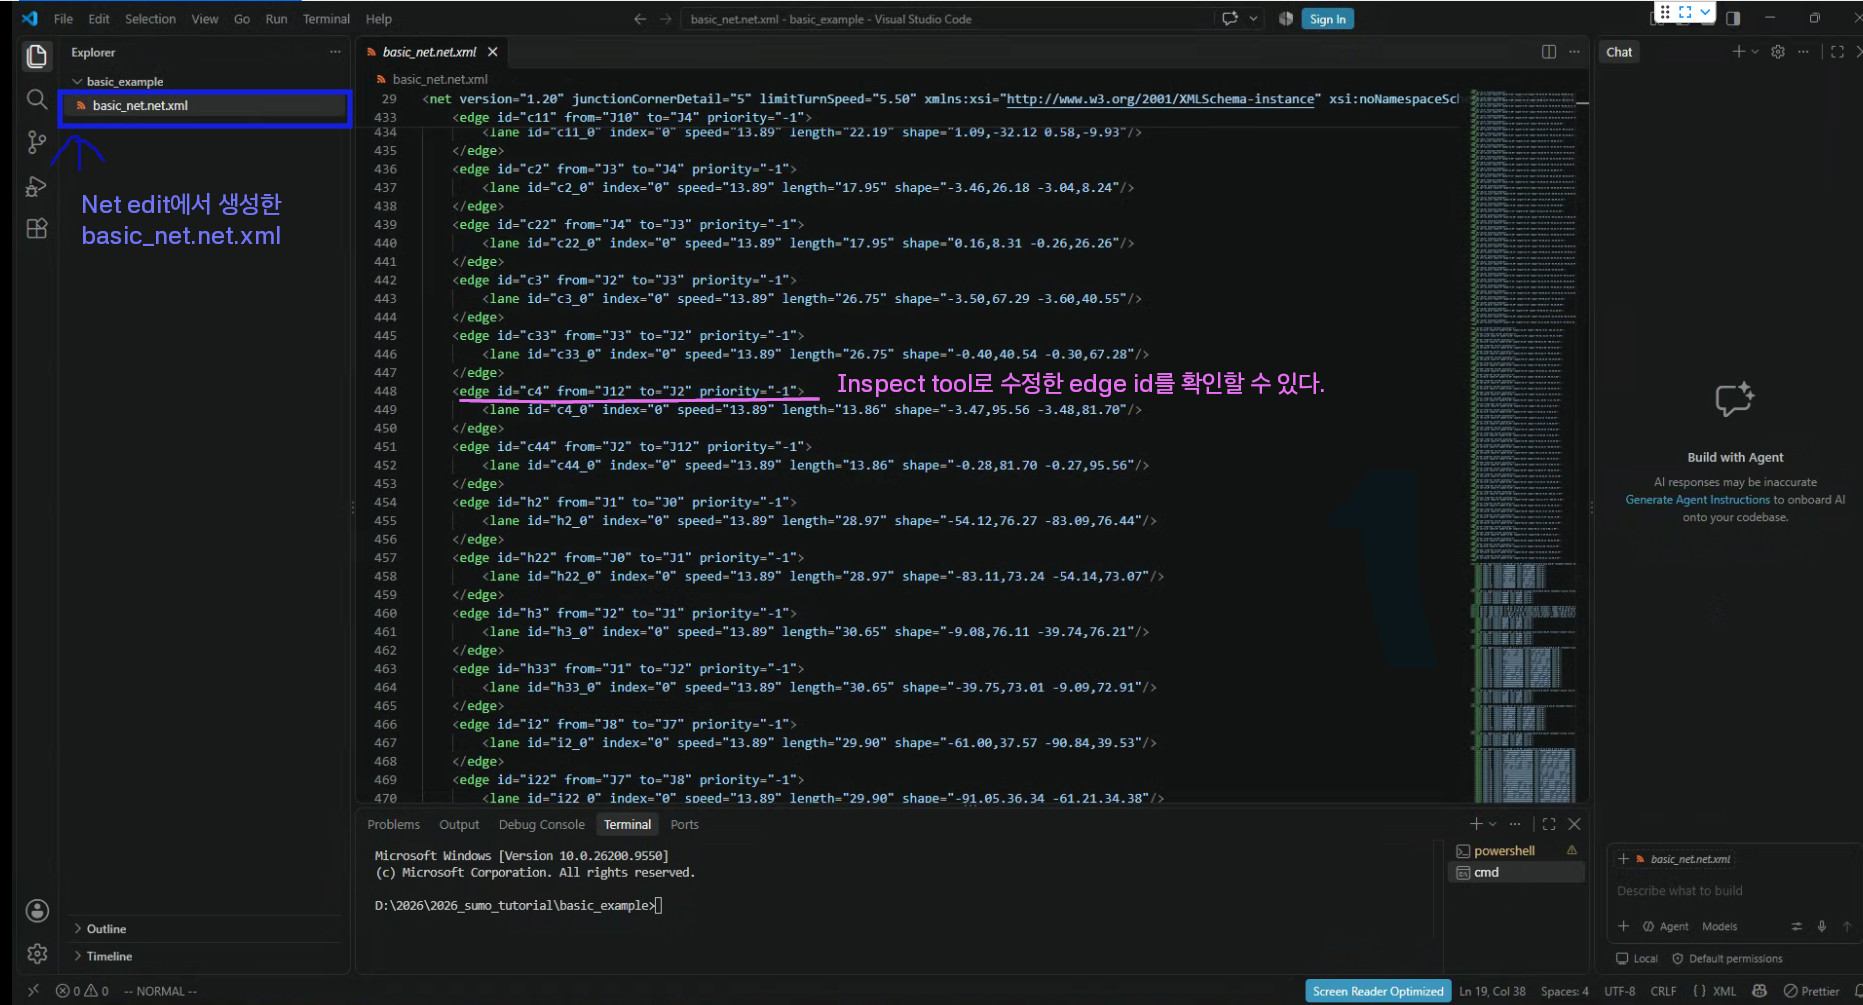
\includegraphics[keepaspectratio]{image/basic_4.jpeg}}
\end{enumerate}

\chapter{신호 입력하기}\label{uxc2e0uxd638-uxc785uxb825uxd558uxae30}

\begin{enumerate}
\def\labelenumi{\arabic{enumi}.}
\tightlist
\item
  traffic light mode를 클릭하고, 교차로(Junction)을 선택하면 신호를
  생성할 수 있다. 아래 그림과 같이 신호를 생성해봅시다.

  \begin{itemize}
  \item
    그림
    \pandocbounded{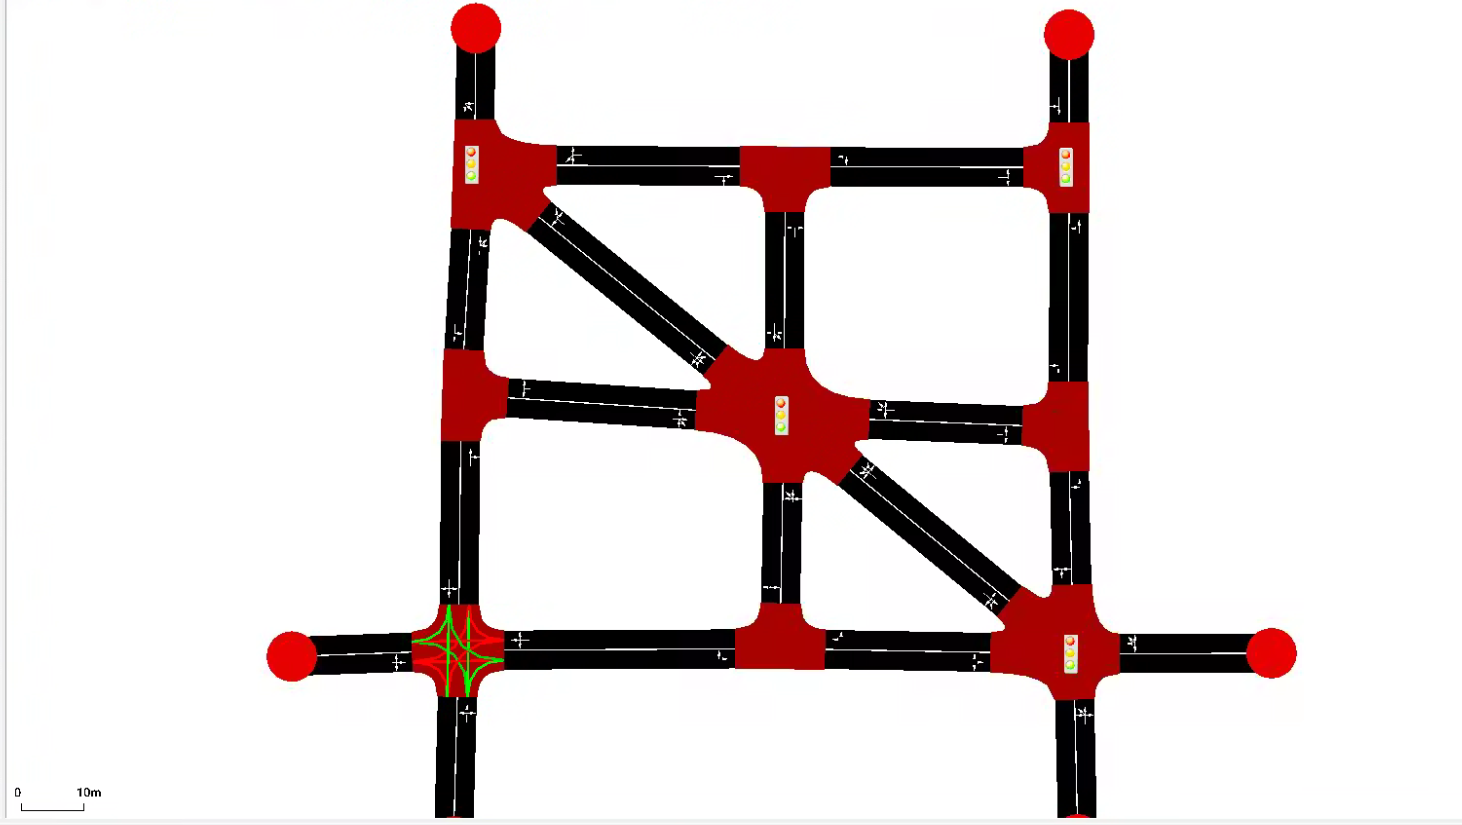
\includegraphics[keepaspectratio]{image/basic_traffic_01.png}}
  \item
    영상
    \pandocbounded{\includegraphics[keepaspectratio]{image/sign.gif}}
  \end{itemize}
\item
  좌측 \texttt{Edit\ Traffic\ Light} 패널의 Phases에서 신호 현시를
  설정할 수 있다.
\end{enumerate}

각 소문자는 교차로에서 lane-lane 간의 신호 상태를 의미한다. 시계 방향
순으로 정렬된다. r을 빨간불, g는 비보호 초록불, y는 노란불, G은
초록불이다.

Offset을 통해 신호 간 시간 간격을 설정할 수 있다.

\pandocbounded{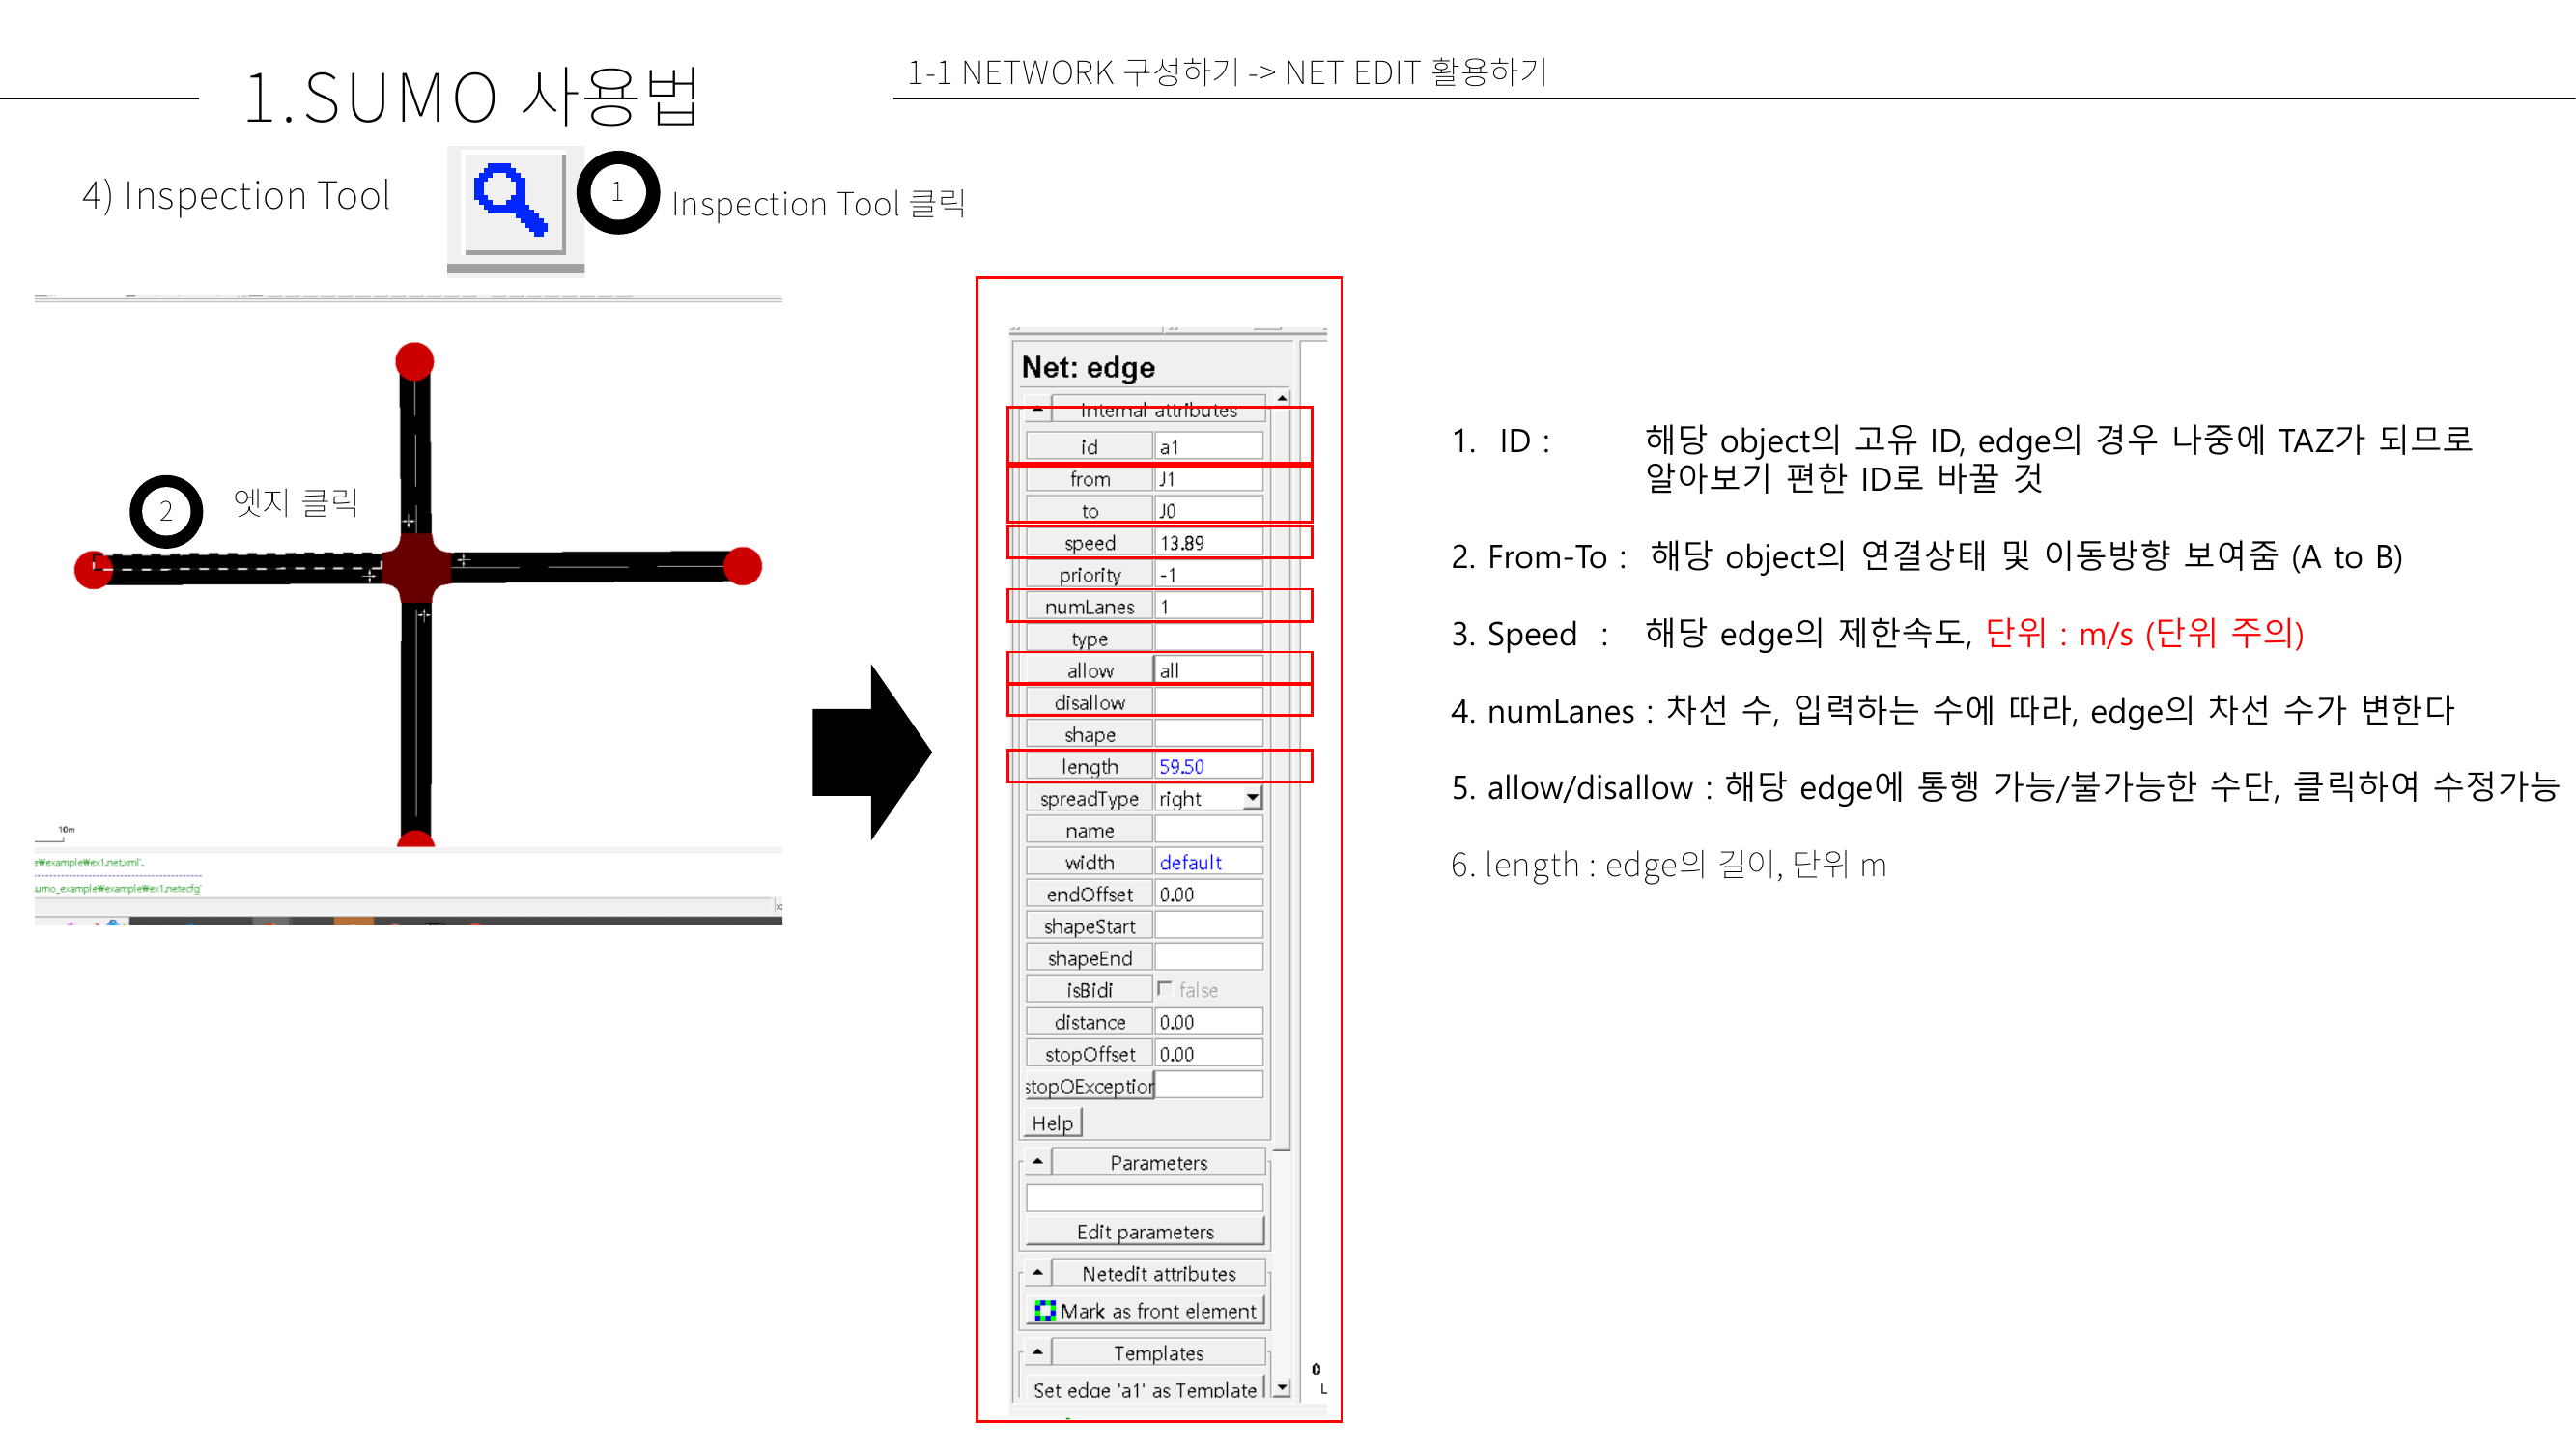
\includegraphics[keepaspectratio]{image/page-17.png}}

\begin{enumerate}
\def\labelenumi{\arabic{enumi}.}
\setcounter{enumi}{2}
\tightlist
\item
  더 궁금한 것이 있다면
  \href{https://sumo.dlr.de/docs/Simulation/Traffic_Lights.html}{sumo
  document - traffic lights}을 참고하시기 바랍니다.
\end{enumerate}

\chapter{교통 수요 생성}\label{uxad50uxd1b5-uxc218uxc694-uxc0dduxc131}

도로 위를 지나는 차량은 이 네트워크에 대한 교통 수요라고 볼 수 있습니다.
교통 수요를 SUMO에 입력하면, 특정 교통 수요가 발생했을 때의
네트워크에서의 교통 흐름을 볼 수 있습니다.

교통 흐름을 보기 위해서는 우선 교통 수요를 추정해야합니다. 교통 수요는
4단계로 추정합니다. ==통행 발생, 통행 분포, 수단 선택, 통행
배정==입니다.

우선 기본 예제 에서는 이미 수단이 차량으로 선택되어 있기 때문에, 차량의
통행 발생, 통행 분포, 통행 배정의 결과를 추정하면 됩니다. 이 추정 결과를
SUMO에 입력하면 차량 시뮬레이을 볼 수 있습니다.

SUMO는 통행 발생, 통행 분포, 노선 배정을 할 수 있는 프로그램을
제공합니다.

이번 기본 실습에서는 차량 통행 발생, 차량 통행 분포, 차량 통행 배정 즉
노선 배정(routing)을 해 보겠습니다.

\section{통행 발생, 통행 분포
생성}\label{uxd1b5uxd589-uxbc1cuxc0dd-uxd1b5uxd589-uxbd84uxd3ec-uxc0dduxc131}

sumo에서는 차량 통행 발생과 통행 분포를 \texttt{od2trips} 프로그램으로
수행할 수 있습니다. OD matrix 파일을 만들고, 이 파일을 od2trips에
넣어주면, OD matrix에 맞춰 차량 통행을 생성할 수 있습니다.

\subsection{TAZ 정의}\label{taz-uxc815uxc758}

OD matrix를 만들기 전에 우선, 이 OD가 되는 TAZ(Traffic Analysix Zone)을
설정해야합니다. sumo에서 taz는 edge들의 합으로 구성됩니다. 그러므로,
개별 edge를 taz로 만들어도 되고, 여러개의 edge를 묶어서 하나의 TAZ로
구성할 수 있습니다.

이번 실습에서는 아래 그림과 같이 4개의 TAZ를 구성해보겠습니다.
\pandocbounded{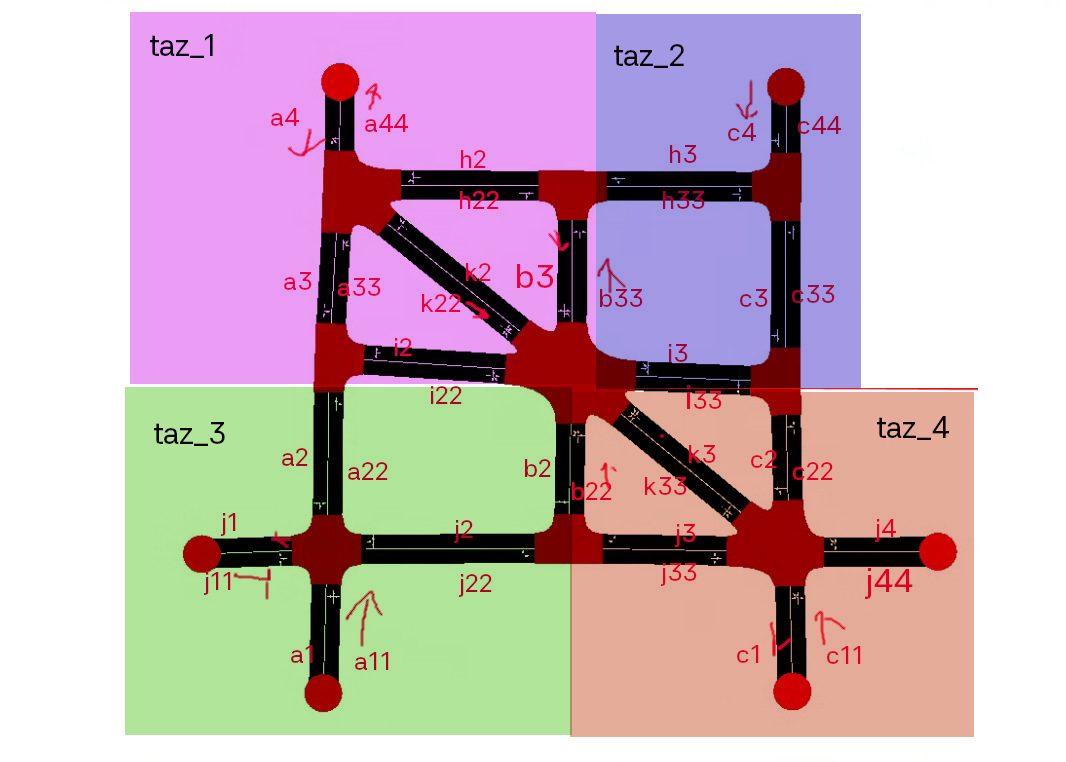
\includegraphics[keepaspectratio,alt={taz 정의}]{image/taz_define.jpeg}}

SUMO에서 TAZ 정의는 \texttt{taz.xml}파일을 통해 정의 할 수 있습니다. TAZ
정의 파일명 : \texttt{basic\_taz.taz.xml}

\begin{enumerate}
\def\labelenumi{\arabic{enumi}.}
\item
  vs code에서 프로젝트 폴더 열기 -\textgreater{} 프로젝트 폴더 옆
  \texttt{New\ File\ 아이콘\ 클릭} 혹은
  \texttt{오른쪽\ 마우스\ 클릭\ \textgreater{}\ New\ File\textquotesingle{}클릭\ -\textgreater{}\ 파일명}basic\_taz.taz.xml`입력
  \pandocbounded{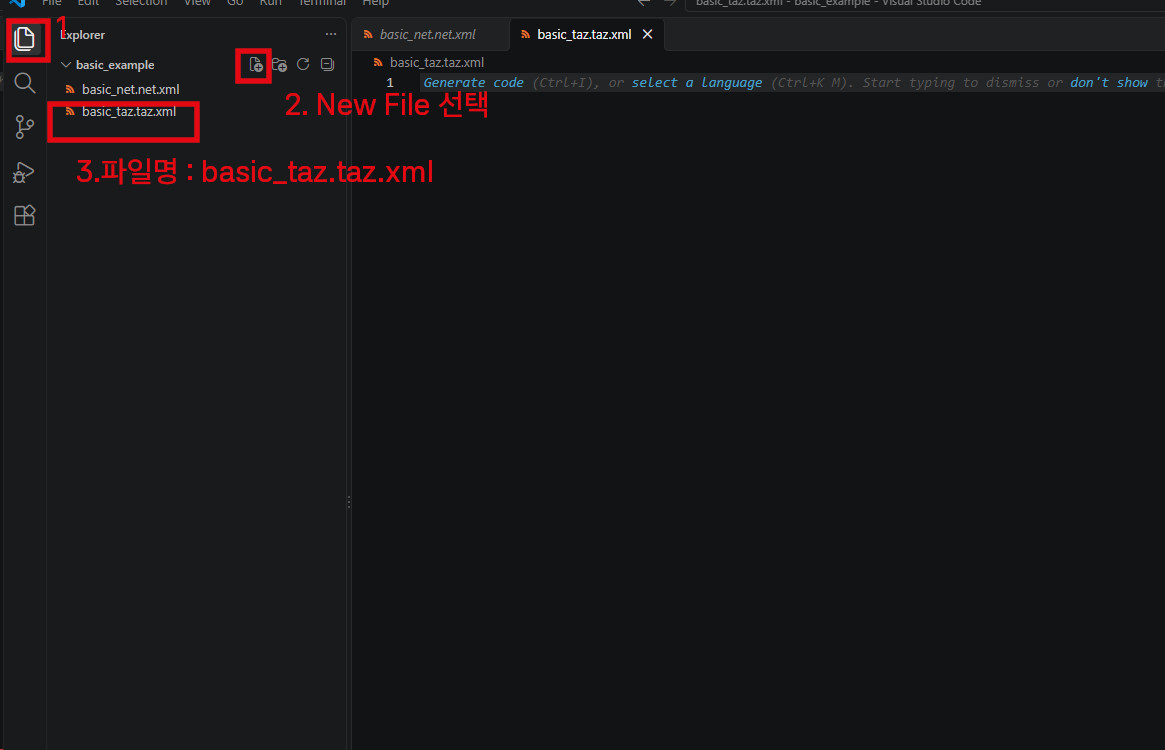
\includegraphics[keepaspectratio]{image/taz_02.jpeg}}
\item
  위 \textbf{taz 정의} 그림과 같이 taz와 edge 연결 관계 정의하기 위해
  xml 파일을 아래와 같이 작성하고 파일을 저장합니다. taz의 입구 도로,
  출구 도로를 각각 source와 sink로 표기합니다. source edge와 sink edge를
  정의하지 않으면, od2trips에서 도로 연결 관계에 맞지 않은 통행을
  생성하게 되고, 이 통행에 경로를 배정할 수 없어 시뮬레이션을 진행할 수
  없게 됩니다. sink, source 표기를 통해 도로의 연결 관계를 반영하여
  통행을 생성할 수 있습니다.
\end{enumerate}

\begin{Shaded}
\begin{Highlighting}[]
\NormalTok{\textless{}}\KeywordTok{tazs}\NormalTok{\textgreater{}}
\NormalTok{    \textless{}}\KeywordTok{taz} \OtherTok{id=}\StringTok{"taz\_1"}\NormalTok{\textgreater{} }
    \CommentTok{\textless{}!{-}{-} taz input edge 정의 {-}{-}\textgreater{}}
\NormalTok{        \textless{}}\KeywordTok{tazSource} \OtherTok{id=}\StringTok{"a33"} \OtherTok{weight} \OtherTok{=}\StringTok{"1"}\NormalTok{/\textgreater{}}
\NormalTok{        \textless{}}\KeywordTok{tazSource} \OtherTok{id=}\StringTok{"a4"} \OtherTok{weight} \OtherTok{=}\StringTok{"1"}\NormalTok{/\textgreater{}}
\NormalTok{        \textless{}}\KeywordTok{tazSource} \OtherTok{id=}\StringTok{"h2"} \OtherTok{weight=}\StringTok{"1"}\NormalTok{/\textgreater{}}
\NormalTok{        \textless{}}\KeywordTok{tazSource} \OtherTok{id=}\StringTok{"k2"} \OtherTok{weight=}\StringTok{"1"}\NormalTok{/\textgreater{}}
\NormalTok{        \textless{}}\KeywordTok{tazSource} \OtherTok{id=}\StringTok{"i2"} \OtherTok{weight=}\StringTok{"1"}\NormalTok{/\textgreater{}}
\NormalTok{        \textless{}}\KeywordTok{tazSource} \OtherTok{id=}\StringTok{"b33"} \OtherTok{weight=}\StringTok{"1"}\NormalTok{/\textgreater{}}
    \CommentTok{\textless{}!{-}{-} taz output edge 정의 {-}{-}\textgreater{}}
\NormalTok{        \textless{}}\KeywordTok{tazSink} \OtherTok{id=}\StringTok{"a3"} \OtherTok{weight=}\StringTok{"1"}\NormalTok{/\textgreater{}}
\NormalTok{        \textless{}}\KeywordTok{tazSink} \OtherTok{id=}\StringTok{"a44"} \OtherTok{weight=}\StringTok{"1"}\NormalTok{/\textgreater{}}
\NormalTok{        \textless{}}\KeywordTok{tazSink} \OtherTok{id=}\StringTok{"h22"} \OtherTok{weight=}\StringTok{"1"}\NormalTok{/\textgreater{}}
\NormalTok{        \textless{}}\KeywordTok{tazSink} \OtherTok{id=}\StringTok{"k22"} \OtherTok{weight=}\StringTok{"1"}\NormalTok{/\textgreater{}}
\NormalTok{        \textless{}}\KeywordTok{tazSink} \OtherTok{id=}\StringTok{"i22"} \OtherTok{weight=}\StringTok{"1"}\NormalTok{/\textgreater{}}
\NormalTok{        \textless{}}\KeywordTok{tazSink} \OtherTok{id=}\StringTok{"b3"} \OtherTok{weight=}\StringTok{"1"}\NormalTok{/\textgreater{}}
\NormalTok{    \textless{}/}\KeywordTok{taz}\NormalTok{\textgreater{}}
\NormalTok{    \textless{}}\KeywordTok{taz} \OtherTok{id=}\StringTok{"taz\_2"}\NormalTok{\textgreater{}}
    \CommentTok{\textless{}!{-}{-} taz input edge 정의 {-}{-}\textgreater{}}
\NormalTok{        \textless{}}\KeywordTok{tazSource} \OtherTok{id=}\StringTok{"c4"} \OtherTok{weight=}\StringTok{"1"}\NormalTok{/\textgreater{}}
\NormalTok{        \textless{}}\KeywordTok{tazSource} \OtherTok{id=}\StringTok{"c33"} \OtherTok{weight=}\StringTok{"1"}\NormalTok{/\textgreater{}}
\NormalTok{        \textless{}}\KeywordTok{tazSource} \OtherTok{id=}\StringTok{"i3"} \OtherTok{weight=}\StringTok{"1"}\NormalTok{/\textgreater{}}
\NormalTok{        \textless{}}\KeywordTok{tazSource} \OtherTok{id=}\StringTok{"h33"} \OtherTok{weight=}\StringTok{"1"}\NormalTok{/\textgreater{}}
    \CommentTok{\textless{}!{-}{-} taz output edge 정의 {-}{-}\textgreater{}}
\NormalTok{        \textless{}}\KeywordTok{tazSink} \OtherTok{id=} \StringTok{"c44"} \OtherTok{weight=}\StringTok{"1"}\NormalTok{/\textgreater{}}
\NormalTok{        \textless{}}\KeywordTok{tazSink} \OtherTok{id=} \StringTok{"c3"} \OtherTok{weight=}\StringTok{"1"}\NormalTok{/\textgreater{}}
\NormalTok{        \textless{}}\KeywordTok{tazSink} \OtherTok{id=} \StringTok{"i33"} \OtherTok{weight=}\StringTok{"1"}\NormalTok{/\textgreater{}}
\NormalTok{        \textless{}}\KeywordTok{tazSink} \OtherTok{id=} \StringTok{"h3"} \OtherTok{weight=}\StringTok{"1"}\NormalTok{/\textgreater{}}
\NormalTok{    \textless{}/}\KeywordTok{taz}\NormalTok{\textgreater{}}
\NormalTok{    \textless{}}\KeywordTok{taz} \OtherTok{id} \OtherTok{=}\StringTok{"taz\_3"}\NormalTok{\textgreater{}}
    \CommentTok{\textless{}!{-}{-} taz input edge 정의 {-}{-}\textgreater{}}
\NormalTok{        \textless{}}\KeywordTok{tazSource} \OtherTok{id=}\StringTok{"a2"} \OtherTok{weight=}\StringTok{"1"}\NormalTok{/\textgreater{}}
\NormalTok{        \textless{}}\KeywordTok{tazSource} \OtherTok{id=}\StringTok{"a11"} \OtherTok{weight=}\StringTok{"1"}\NormalTok{/\textgreater{}}
\NormalTok{        \textless{}}\KeywordTok{tazSource} \OtherTok{id=}\StringTok{"j11"} \OtherTok{weight=}\StringTok{"1"}\NormalTok{/\textgreater{}}
\NormalTok{        \textless{}}\KeywordTok{tazSource} \OtherTok{id=}\StringTok{"j2"} \OtherTok{weight=}\StringTok{"1"}\NormalTok{/\textgreater{}}
\NormalTok{        \textless{}}\KeywordTok{tazSource} \OtherTok{id=}\StringTok{"b2"} \OtherTok{weight=}\StringTok{"1"}\NormalTok{/\textgreater{}}
    \CommentTok{\textless{}!{-}{-} taz output edge 정의 {-}{-}\textgreater{}}
\NormalTok{        \textless{}}\KeywordTok{tazSink} \OtherTok{id=} \StringTok{"a22"} \OtherTok{weight=}\StringTok{"1"}\NormalTok{/\textgreater{}}
\NormalTok{        \textless{}}\KeywordTok{tazSink} \OtherTok{id=} \StringTok{"a1"} \OtherTok{weight=}\StringTok{"1"}\NormalTok{/\textgreater{}}
\NormalTok{        \textless{}}\KeywordTok{tazSink} \OtherTok{id=} \StringTok{"j1"} \OtherTok{weight=}\StringTok{"1"}\NormalTok{/\textgreater{}}
\NormalTok{        \textless{}}\KeywordTok{tazSink} \OtherTok{id=}\StringTok{"j22"} \OtherTok{weight=}\StringTok{"1"}\NormalTok{/\textgreater{}}
\NormalTok{    \textless{}/}\KeywordTok{taz}\NormalTok{\textgreater{}}
\NormalTok{    \textless{}}\KeywordTok{taz} \OtherTok{id} \OtherTok{=}\StringTok{"taz\_4"}\NormalTok{\textgreater{}}
    \CommentTok{\textless{}!{-}{-} taz input edge 정의 {-}{-}\textgreater{}}
\NormalTok{        \textless{}}\KeywordTok{tazSource} \OtherTok{id=} \StringTok{"c11"} \OtherTok{weight=}\StringTok{"1"}\NormalTok{/\textgreater{}}
\NormalTok{        \textless{}}\KeywordTok{tazSource} \OtherTok{id=} \StringTok{"j4"} \OtherTok{weight=}\StringTok{"1"}\NormalTok{/\textgreater{}}
\NormalTok{        \textless{}}\KeywordTok{tazSource} \OtherTok{id=} \StringTok{"k33"} \OtherTok{weight=}\StringTok{"1"}\NormalTok{/\textgreater{}}
\NormalTok{        \textless{}}\KeywordTok{tazSource} \OtherTok{id=} \StringTok{"c2"} \OtherTok{weight=}\StringTok{"1"}\NormalTok{/\textgreater{}}
    \CommentTok{\textless{}!{-}{-} taz output edge 정의 {-}{-}\textgreater{}}
\NormalTok{        \textless{}}\KeywordTok{tazSink} \OtherTok{id=} \StringTok{"c1"} \OtherTok{weight=}\StringTok{"1"}\NormalTok{/\textgreater{}}
\NormalTok{        \textless{}}\KeywordTok{tazSink} \OtherTok{id=} \StringTok{"j44"} \OtherTok{weight=}\StringTok{"1"}\NormalTok{/\textgreater{}}
\NormalTok{        \textless{}}\KeywordTok{tazSink} \OtherTok{id=} \StringTok{"k3"} \OtherTok{weight=}\StringTok{"1"}\NormalTok{/\textgreater{}}
\NormalTok{        \textless{}}\KeywordTok{tazSink} \OtherTok{id=} \StringTok{"c22"} \OtherTok{weight=}\StringTok{"1"}\NormalTok{/\textgreater{}}
\NormalTok{        \textless{}}\KeywordTok{tazSink} \OtherTok{id=} \StringTok{"b22"} \OtherTok{weight=}\StringTok{"1"}\NormalTok{/\textgreater{}}
\NormalTok{    \textless{}/}\KeywordTok{taz}\NormalTok{\textgreater{}}
\NormalTok{\textless{}/}\KeywordTok{tazs}\NormalTok{\textgreater{}}
\end{Highlighting}
\end{Shaded}

\pandocbounded{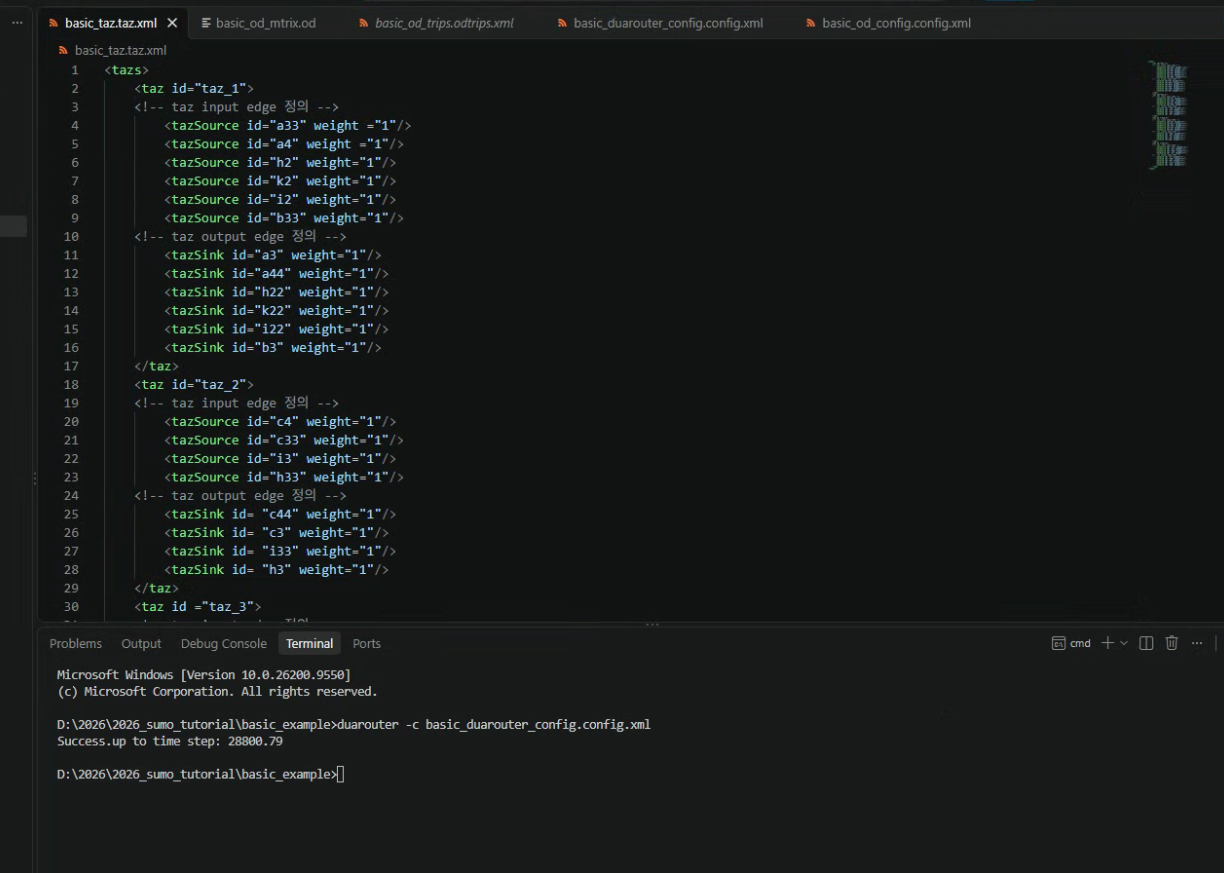
\includegraphics[keepaspectratio]{image/taz_03.png}}

\subsection{OD matrix 정의}\label{od-matrix-uxc815uxc758}

아래 그림 파란색 화살표와 숫자를 차량의 이동이라고 합시다.

\pandocbounded{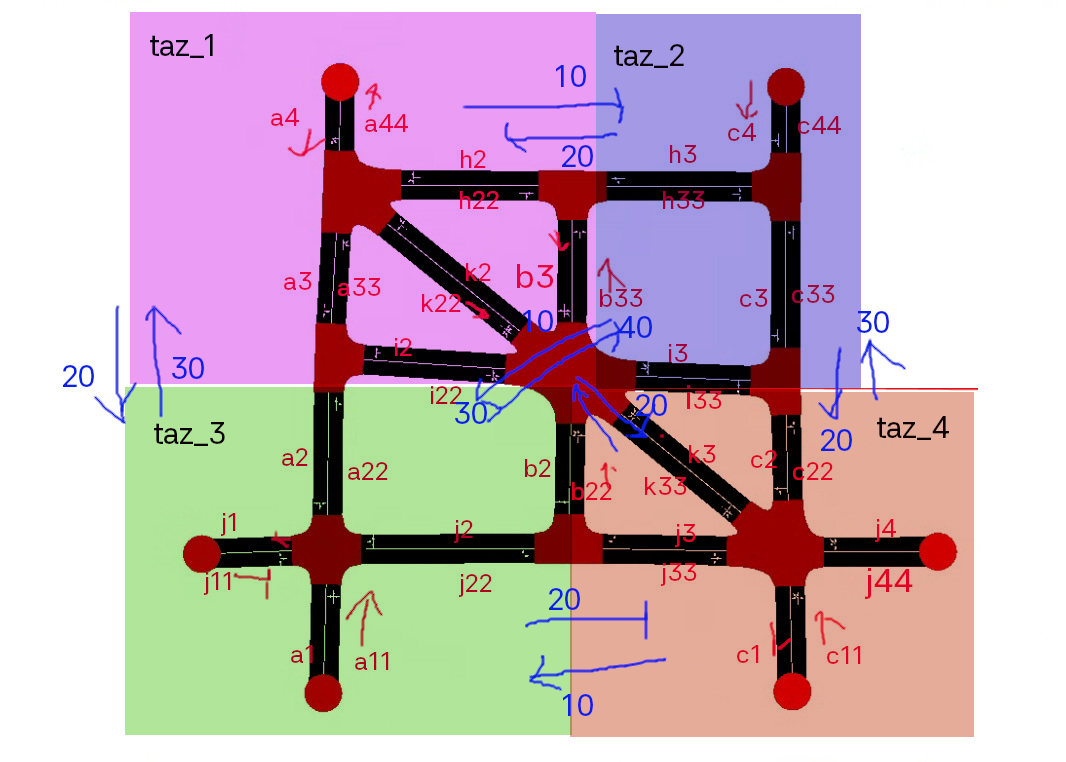
\includegraphics[keepaspectratio]{image/taz_04.png}}

이와 같은 OD 차량 흐름을 표로 정리할 수 있습니다.

{\def\LTcaptype{none} % do not increment counter
\begin{longtable}[]{@{}llr@{}}
\toprule\noalign{}
O & D & car volume \\
\midrule\noalign{}
\endhead
\bottomrule\noalign{}
\endlastfoot
taz\_1 & taz\_2 & 10.00 \\
taz\_1 & taz\_3 & 20.00 \\
taz\_1 & taz\_4 & 20.00 \\
taz\_2 & taz\_1 & 20.00 \\
taz\_2 & taz\_3 & 30.00 \\
taz\_2 & taz\_4 & 20.00 \\
taz\_3 & taz\_1 & 30.00 \\
taz\_3 & taz\_2 & 40.00 \\
taz\_3 & taz\_4 & 20.00 \\
taz\_4 & taz\_1 & 10.00 \\
taz\_4 & taz\_2 & 30.00 \\
taz\_4 & taz\_3 & 10.00 \\
\end{longtable}
}

이 표를 od2trips가 읽을 수 있는 od matrix 파일로 작성해봅시다.

\begin{enumerate}
\def\labelenumi{\arabic{enumi}.}
\tightlist
\item
  vscode 열기 \textgreater{} 새파일 \textgreater{} 파일명
  \texttt{basic\_od\_matrix.od} 작성
\item
  아래의 od matrix 파일을 입력하고 파일 저장
\end{enumerate}

\begin{verbatim}
$OR;D2
* From-Time  To-Time
0.00 1.00
* Factor
1.00
* some
* additional
* comments
        taz_1      taz_2      10.00
        taz_1      taz_3      20.00
        taz_1      taz_4      20.00
        taz_2      taz_1      20.00
        taz_2      taz_3      30.00
        taz_2      taz_4      20.00
        taz_3      taz_1      30.00
        taz_3      taz_2      40.00
        taz_3      taz_4      20.00
        taz_4      taz_1      10.00
        taz_4      taz_2      30.00
        taz_4      taz_3      10.00
\end{verbatim}

\pandocbounded{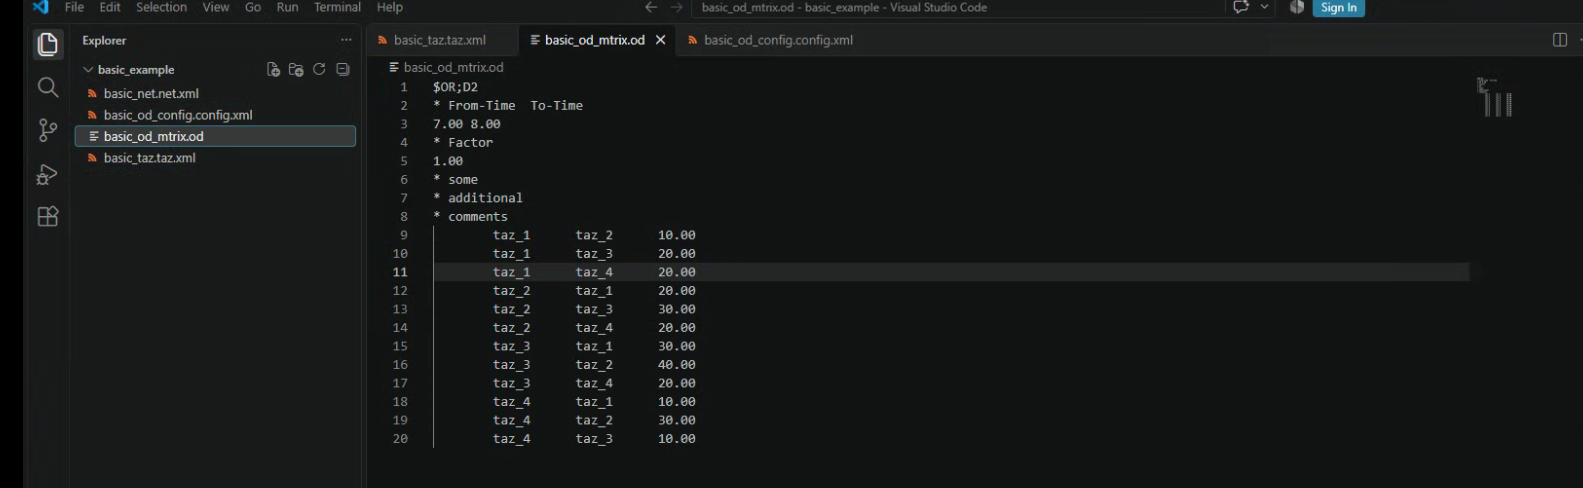
\includegraphics[keepaspectratio]{image/od_matrix.png}}

코드 설명

{\def\LTcaptype{none} % do not increment counter
\begin{longtable}[]{@{}ll@{}}
\toprule\noalign{}
줄 & 의미 \\
\midrule\noalign{}
\endhead
\bottomrule\noalign{}
\endlastfoot
\texttt{\$OR;D2} & PTV O-format 매트릭스 \\
\texttt{0.00\ 1.00} & 시뮬레이션 시작·종료 시각 1시간 시뮬레이션 \\
\texttt{1.00} & car volume에 곱하는 scale 상수 \\
\texttt{taz\_1\ taz\_2\ 10.00} & 출발 TAZ, 도착 TAZ, 차량 수 \\
* & 주석 표기 \\
\end{longtable}
}

\emph{상세한 matrix 파일 설명은
\href{https://sumo.dlr.de/docs/Demand/Importing_O/D_Matrices.html}{sumo
document - od matrix \textgreater{} PTV formats}에서 확인하실 수
있습니다.}

\subsection{od2trips configuration 파일
작성}\label{od2trips-configuration-uxd30cuxc77c-uxc791uxc131}

taz 정의와 od matrix 정의를 od2trips 프로그램에 전달하면, od2trips
프로그램을 통해 차량 통행 파일 trips을 생성할 수 있습니다. 이런 입력
파일과 결과 파일을 어떻게 od2trips에 입력할 수 있을까요? configuration
파일을 통해 od2trips의 입력, 결과 파일을 전달 할 수 있습니다.
configuration은 설정을 의미하며, od2trips 프로그램 설정을 xml로 작성한
것입니다.

\begin{enumerate}
\def\labelenumi{\arabic{enumi}.}
\tightlist
\item
  vs code 열기 \textgreater{} 새 파일 \textgreater{} 파일명
  \texttt{basic\_od\_config.config.xml} 입력
\item
  아래와 같이 od2trips configuration을 입력하고 파일 저장
\end{enumerate}

\begin{Shaded}
\begin{Highlighting}[]
\NormalTok{\textless{}}\KeywordTok{configuration}\NormalTok{\textgreater{}}
\CommentTok{\textless{}!{-}{-} od2trips input 파일 정의 {-}{-}\textgreater{}}
\NormalTok{    \textless{}}\KeywordTok{input}\NormalTok{\textgreater{}}
        \CommentTok{\textless{}!{-}{-} taz 파일 입력 {-}{-}\textgreater{}}
\NormalTok{        \textless{}}\KeywordTok{taz{-}files} \OtherTok{value=}\StringTok{"basic\_taz.taz.xml"}\NormalTok{/\textgreater{}}
        \CommentTok{\textless{}!{-}{-} od maatrix 파일 입력 {-}{-}\textgreater{}}
\NormalTok{        \textless{}}\KeywordTok{od{-}matrix{-}files} \OtherTok{value=}\StringTok{"basic\_od\_mtrix.od"}\NormalTok{/\textgreater{}}
\NormalTok{    \textless{}/}\KeywordTok{input}\NormalTok{\textgreater{}}
\CommentTok{\textless{}!{-}{-} od2trips output 파일 정의 {-}{-}\textgreater{}}
\NormalTok{    \textless{}}\KeywordTok{output}\NormalTok{\textgreater{}}
        \CommentTok{\textless{}!{-}{-} 차량 통행 파일명 정의, od2trips를 실행하고 나면, 그 결과물로 산출되는 차량 통행이 이 파일명으로 나타난다. {-}{-}\textgreater{}}
\NormalTok{        \textless{}}\KeywordTok{output{-}file} \OtherTok{value=}\StringTok{"basic\_od\_trips.odtrips.xml"}\NormalTok{/\textgreater{}}
\NormalTok{    \textless{}/}\KeywordTok{output}\NormalTok{\textgreater{}}
\NormalTok{\textless{}/}\KeywordTok{configuration}\NormalTok{\textgreater{}}
\end{Highlighting}
\end{Shaded}

\pandocbounded{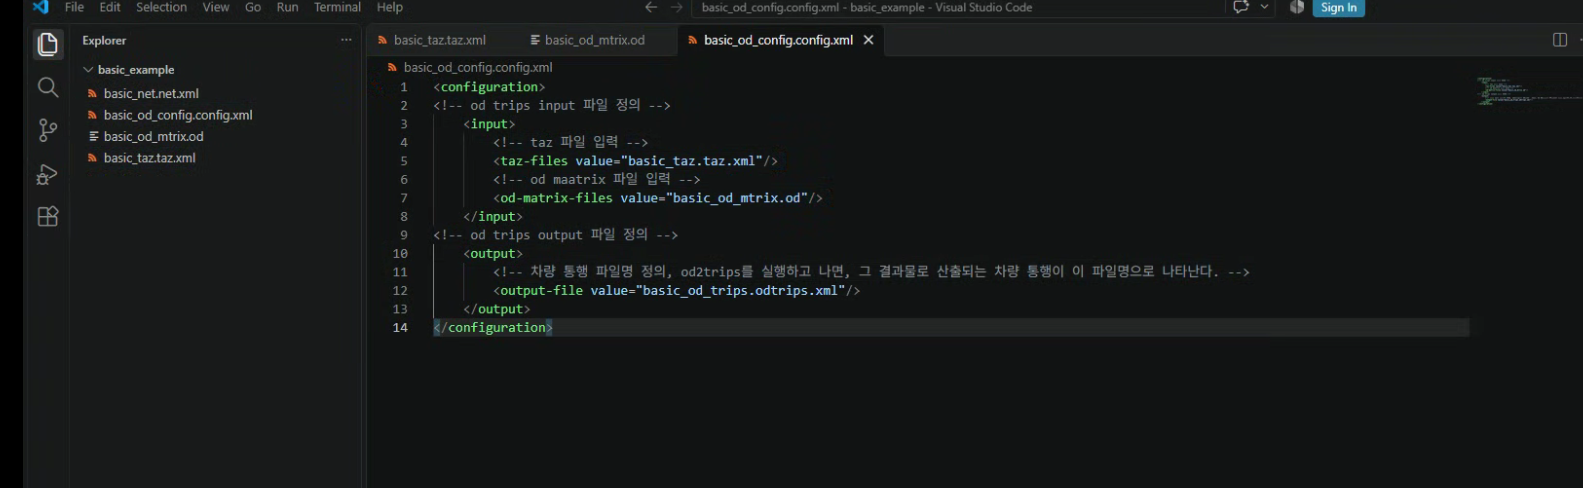
\includegraphics[keepaspectratio]{image/od_config.png}}

상세한 od2trips의 configuration 속성값은
\href{https://sumo.dlr.de/docs/od2trips.html}{sumo document
od2trips}에서 확인할 수 있습니다.

\subsection{od2trips 차량 통행
생성하기}\label{od2trips-uxcc28uxb7c9-uxd1b5uxd589-uxc0dduxc131uxd558uxae30}

\begin{enumerate}
\def\labelenumi{\arabic{enumi}.}
\tightlist
\item
  vs code 프로젝트 폴더에서 터미널 열고, cmd 켜기
  (\texttt{\textasciigrave{}ctrl+\textasciigrave{}}) 아래 명령어 입력
\end{enumerate}

\begin{Shaded}
\begin{Highlighting}[]
\NormalTok{od2trips }\AttributeTok{{-}c}\NormalTok{ basic\_od\_config.config.xml}
\end{Highlighting}
\end{Shaded}

\pandocbounded{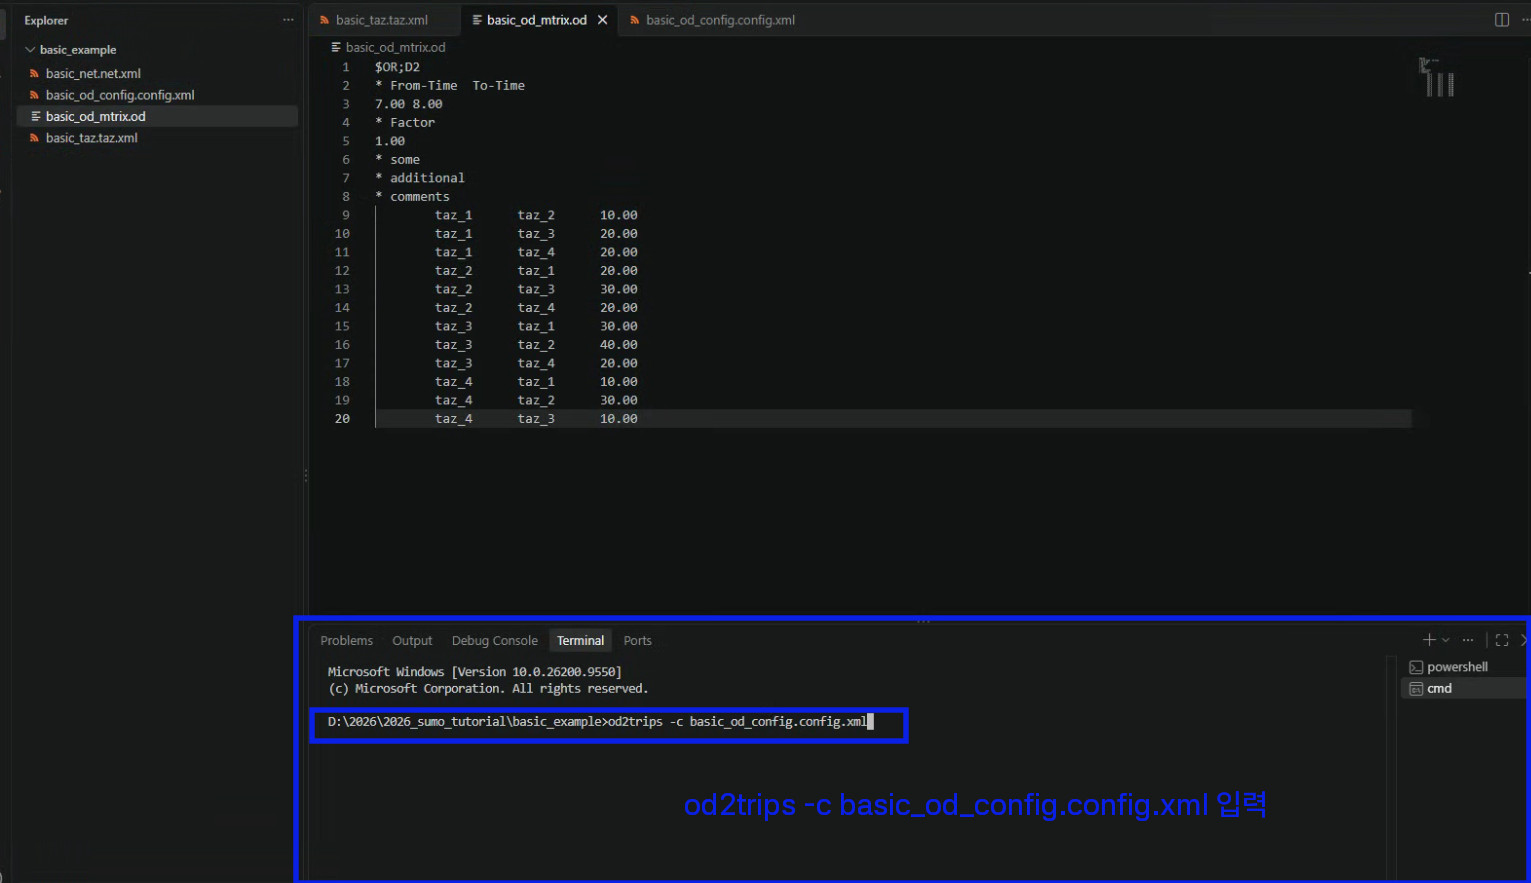
\includegraphics[keepaspectratio]{image/od2trips.jpeg}}

\begin{enumerate}
\def\labelenumi{\arabic{enumi}.}
\setcounter{enumi}{1}
\tightlist
\item
  od2trips 프로그램이 성공하면, configuration에서 정의하였던 산출물 차량
  통행 파일 \texttt{basic\_od\_trips.odtrips.xml}이 나타난다. 이로서
  통행이 생성되었다!
\end{enumerate}

\pandocbounded{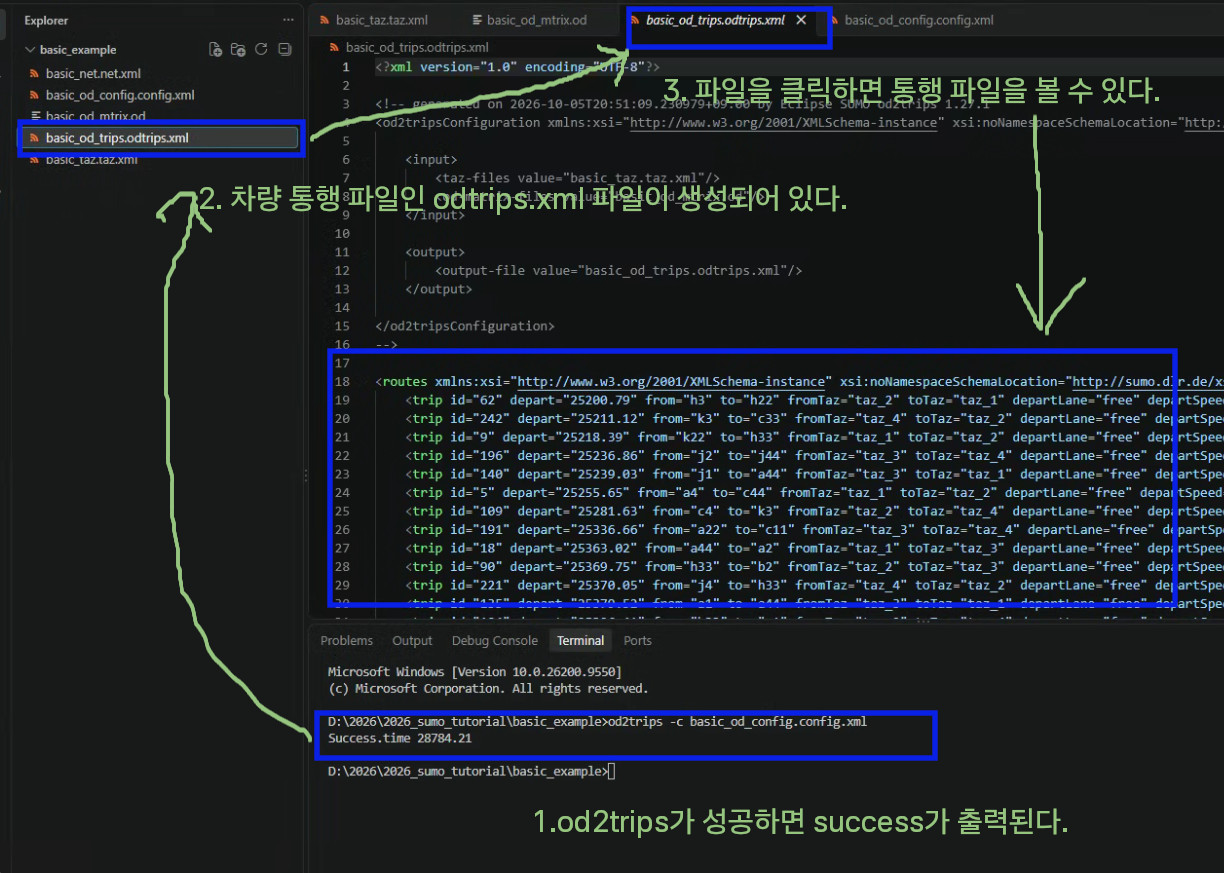
\includegraphics[keepaspectratio]{image/od2trips_result.jpeg}}

\begin{enumerate}
\def\labelenumi{\arabic{enumi}.}
\setcounter{enumi}{2}
\tightlist
\item
  \texttt{basic\_od\_trips.odtrips.xml} 파일에 나타난 통행을 해석할 수
  있다. 만약 통행 즉 \texttt{trip}이 아래의 코드와 같의 나타나있다면,
  이는 id 62 통행이 0초에 h3에서 출발해서 h22로 같나든 것이다. 출발
  taz는 taz\_2이고, 종료 taz는 h22가 속한 taz\_1이다. 이와 같이
  od2trips로 생성한 통행은 출발시각, 출발지, 목적지만 나타나있고, 그
  경로는 나타나있지 않다. 고로, 다음 작업은 각 통행에 경로를 배정하는
  일입니다.
\end{enumerate}

\begin{Shaded}
\begin{Highlighting}[]
\NormalTok{    \textless{}}\KeywordTok{trip} \OtherTok{id=}\StringTok{"62"} \OtherTok{depart=}\StringTok{"0"} \OtherTok{from=}\StringTok{"c4"} \OtherTok{to=}\StringTok{"k22"} \OtherTok{fromTaz=}\StringTok{"taz\_2"} \OtherTok{toTaz=}\StringTok{"taz\_1"} \OtherTok{departLane=}\StringTok{"free"} \OtherTok{departSpeed=}\StringTok{"max"}\NormalTok{/\textgreater{}}
\end{Highlighting}
\end{Shaded}

\section{통행에 경로 배정
하기}\label{uxd1b5uxd589uxc5d0-uxacbduxb85c-uxbc30uxc815-uxd558uxae30}

sumo에서는 경로를 배정하는 여러가지 프로그램을 제공합니다. 이번 기초
실습에서는 \textbf{duarouter}를 이용하여 경로를 배정합니다. duarouter는
통행에 최단 경로를 배정하는 프로그램입니다. duarouter 이외에도 많은 경로
배정 방법이 있습니다만, 이는 tutorial의 범위를 넘어서서 다루지 않습니다.
심화사항은
\href{https://sumo.dlr.de/docs/Demand/Introduction_to_demand_modelling_in_SUMO.html}{sumo
documentation - introduction to demand modeling in sumo}에서 확인하실 수
있습니다.

\textbf{duarouter}도 \textbf{od2trips}와 동일하게 configuration 파일을
통해, 입력, 결과 파일을 정의할 수 있습니다.

\begin{enumerate}
\def\labelenumi{\arabic{enumi}.}
\item
  vscode 열기 \textgreater{} new file \textgreater{} 파일명:
  \texttt{basic\_duarouter\_config.config.xml} 만들기
\item
  아래의 duarouter configuration 입력한 뒤, 파일 저장
\end{enumerate}

\begin{Shaded}
\begin{Highlighting}[]
\NormalTok{\textless{}}\KeywordTok{configuration}\NormalTok{\textgreater{}}
\CommentTok{\textless{}!{-}{-} duarouter input 파일 정의 {-}{-}\textgreater{}}
\NormalTok{    \textless{}}\KeywordTok{input}\NormalTok{\textgreater{}}
        \CommentTok{\textless{}!{-}{-} network 파일 입력 {-}{-}\textgreater{}}
\NormalTok{        \textless{}}\KeywordTok{net{-}file} \OtherTok{value=}\StringTok{"basic\_net.net.xml"}\NormalTok{/\textgreater{}}
        \CommentTok{\textless{}!{-}{-} routing(경로 배정)이 필요한 od trips(통행) 파일 입력 {-}{-}\textgreater{}}
\NormalTok{        \textless{}}\KeywordTok{route{-}files} \OtherTok{value=}\StringTok{"basic\_od\_trips.odtrips.xml"}\NormalTok{/\textgreater{}}
\NormalTok{    \textless{}/}\KeywordTok{input}\NormalTok{\textgreater{}}
\CommentTok{\textless{}!{-}{-} duarouter output 파일 정의 {-}{-}\textgreater{}}
\NormalTok{    \textless{}}\KeywordTok{output}\NormalTok{\textgreater{}}
        \CommentTok{\textless{}!{-}{-} 산출물인 경로 배정한 통행 파일명 정의{-}{-}\textgreater{}}
\NormalTok{        \textless{}}\KeywordTok{output{-}file} \OtherTok{value=}\StringTok{"basic\_shortest\_routes.rou.xml"}\NormalTok{/\textgreater{}}
\NormalTok{    \textless{}/}\KeywordTok{output}\NormalTok{\textgreater{}}
\CommentTok{\textless{}!{-}{-} duarouter processing option 정의 {-}{-}\textgreater{}}
\NormalTok{    \textless{}}\KeywordTok{processing}\NormalTok{\textgreater{}}
\NormalTok{        \textless{}}\KeywordTok{repair} \OtherTok{value=}\StringTok{"true"}\NormalTok{/\textgreater{}}
\NormalTok{        \textless{}}\KeywordTok{repair.from} \OtherTok{value=}\StringTok{"true"}\NormalTok{/\textgreater{}}
\NormalTok{        \textless{}}\KeywordTok{repair.to} \OtherTok{value=}\StringTok{"true"}\NormalTok{/\textgreater{}}
\NormalTok{    \textless{}/}\KeywordTok{processing}\NormalTok{\textgreater{}}
\NormalTok{\textless{}/}\KeywordTok{configuration}\NormalTok{\textgreater{}}
\end{Highlighting}
\end{Shaded}

\begin{enumerate}
\def\labelenumi{\arabic{enumi}.}
\setcounter{enumi}{2}
\tightlist
\item
  vs code에서 cmd 열기 \textgreater{} 아래 명령어 입력
\end{enumerate}

\begin{Shaded}
\begin{Highlighting}[]
\NormalTok{duarouter }\AttributeTok{{-}c}\NormalTok{ basic\_duarouter\_config.config.xml}
\end{Highlighting}
\end{Shaded}

\pandocbounded{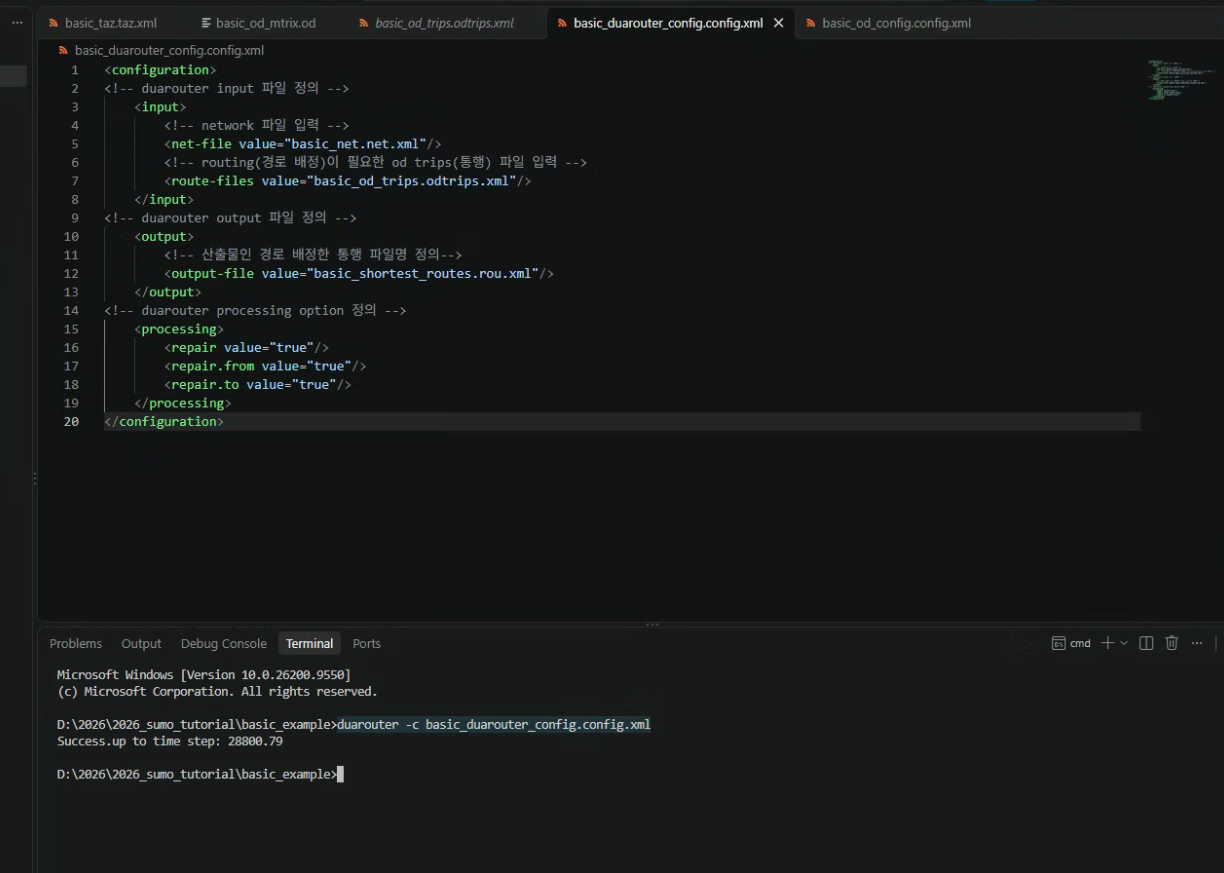
\includegraphics[keepaspectratio]{image/duarouter_succes.png}}

\begin{enumerate}
\def\labelenumi{\arabic{enumi}.}
\setcounter{enumi}{3}
\item
  명령이 성공하면, 폴더 아래 산출물 파일
  \texttt{basic\_shortest\_routes.rou.xml}이 생깁니다.
  \pandocbounded{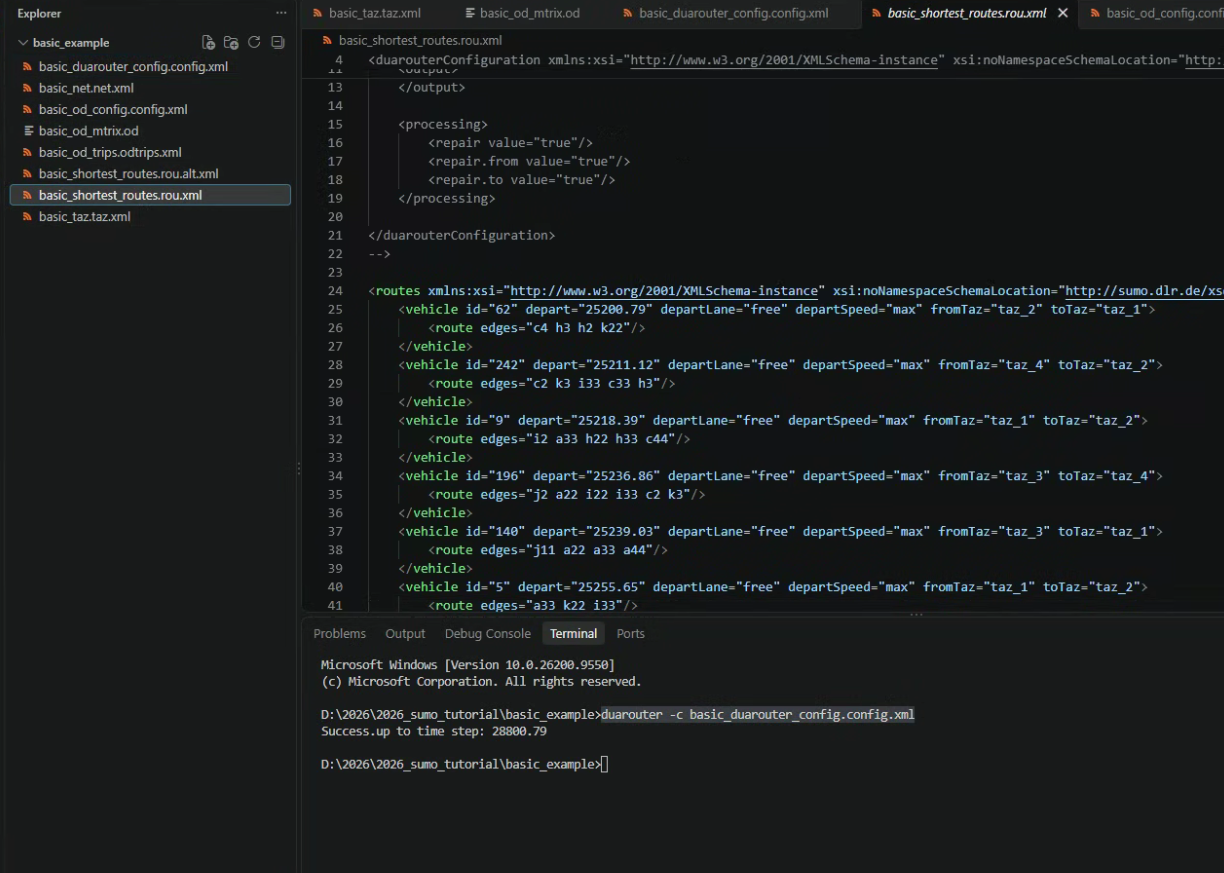
\includegraphics[keepaspectratio]{image/basic_shortest_routes.png}}
\item
  duarouter를 통해 경로가 edge \texttt{c2\ k3\ i33\ c33\ h3}가 통행
  242번에 배정된 것을 확인할 수 있습니다.
\end{enumerate}

\begin{Shaded}
\begin{Highlighting}[]
\NormalTok{\textless{}}\KeywordTok{vehicle} \OtherTok{id=}\StringTok{"242"} \OtherTok{depart=}\StringTok{"0"} \OtherTok{departLane=}\StringTok{"free"} \OtherTok{departSpeed=}\StringTok{"max"} \OtherTok{fromTaz=}\StringTok{"taz\_4"} \OtherTok{toTaz=}\StringTok{"taz\_2"}\NormalTok{\textgreater{}}
\NormalTok{        \textless{}}\KeywordTok{route} \OtherTok{edges=}\StringTok{"c2 k3 i33 c33 h3"}\NormalTok{/\textgreater{}}
\end{Highlighting}
\end{Shaded}

이로써, 드디어 교통 수요를 생성하였습니다!

\chapter{시뮬레이션
하기}\label{uxc2dcuxbbacuxb808uxc774uxc158-uxd558uxae30}

네트워크와 교통 수요를 만들었으니, 이제 시뮬레이션을 하면 됩니다. sumo는
시뮬레이션 엔진 프로그램입니다. sumo를 동작하려면 어떤 네트워크 파일과
교통 수요 파일을 사용할 것인지 정의해줘야합니다. 이또한 od2trips와
duarouter처럼, sumo\_configuration 파일로 정의할 수 있습니다. 또한,
시뮬레이션 이후에 결과 파일을 무엇을 받을지도 정의할 수 있습니다.

\section{sumo configuration
정의하기}\label{sumo-configuration-uxc815uxc758uxd558uxae30}

\begin{enumerate}
\def\labelenumi{\arabic{enumi}.}
\item
  vs code 열기 \textgreater{} 새파일 \textgreater{} 파일명
  \texttt{basic\_sumo\_config.sumocfg} 입력, 확장자 sumocfg여야 합니당!
\item
  파일에 아래 내용 입력
\end{enumerate}

\begin{Shaded}
\begin{Highlighting}[]
\NormalTok{\textless{}}\KeywordTok{configuration}\NormalTok{\textgreater{}}
\NormalTok{    \textless{}}\KeywordTok{input}\NormalTok{\textgreater{} }
    \CommentTok{\textless{}!{-}{-} 네트워크 파일명 {-}{-}\textgreater{}}
\NormalTok{        \textless{}}\KeywordTok{net{-}file} \OtherTok{value=}\StringTok{"basic\_net.net.xml"}\NormalTok{/\textgreater{} }
    \CommentTok{\textless{}!{-}{-} 경로 배정한 파일명 {-}{-}\textgreater{}}
\NormalTok{        \textless{}}\KeywordTok{route{-}files} \OtherTok{value=}\StringTok{"basic\_shortest\_routes.rou.xml"}\NormalTok{/\textgreater{} }
\NormalTok{    \textless{}/}\KeywordTok{input}\NormalTok{\textgreater{} }
\NormalTok{    \textless{}}\KeywordTok{time}\NormalTok{\textgreater{} }
    \CommentTok{\textless{}!{-}{-} 만약 시뮬레이션을 간단하게 하고 싶으면 OD matrix에서 0, 1을 입력하여서, 0, 3600을 여기에 입력하면 됨{-}{-}\textgreater{}}
\NormalTok{        \textless{}}\KeywordTok{begin} \OtherTok{value=}\StringTok{"0"}\NormalTok{/\textgreater{} }
\NormalTok{        \textless{}}\KeywordTok{end} \OtherTok{value=}\StringTok{"3600"}\NormalTok{/\textgreater{} }
\NormalTok{    \textless{}/}\KeywordTok{time}\NormalTok{\textgreater{}}
\NormalTok{    \textless{}}\KeywordTok{output}\NormalTok{\textgreater{}}
    \CommentTok{\textless{}!{-}{-} edge 시뮬레이션 결과 출력{-}{-}\textgreater{}}
\NormalTok{        \textless{}}\KeywordTok{edgedata{-}output} \OtherTok{value=}\StringTok{"edge\_output.xml"}\NormalTok{/\textgreater{}}
    \CommentTok{\textless{}!{-}{-} edge lane 차선 시뮬레이션 결과 출력{-}{-}\textgreater{}}
\NormalTok{        \textless{}}\KeywordTok{lanedata{-}output} \OtherTok{value=}\StringTok{"lane\_output.xml"}\NormalTok{/\textgreater{}}
    \CommentTok{\textless{}!{-}{-} vehicle 별 통행 시뮬레이션 결과 출력{-}{-}\textgreater{}}
\NormalTok{        \textless{}}\KeywordTok{tripinfo{-}output} \OtherTok{value} \OtherTok{=}\StringTok{"trip\_info.xml"}\NormalTok{/\textgreater{}}
\NormalTok{    \textless{}/}\KeywordTok{output}\NormalTok{\textgreater{}}
\NormalTok{\textless{}/}\KeywordTok{configuration}\NormalTok{\textgreater{}}
\end{Highlighting}
\end{Shaded}

\pandocbounded{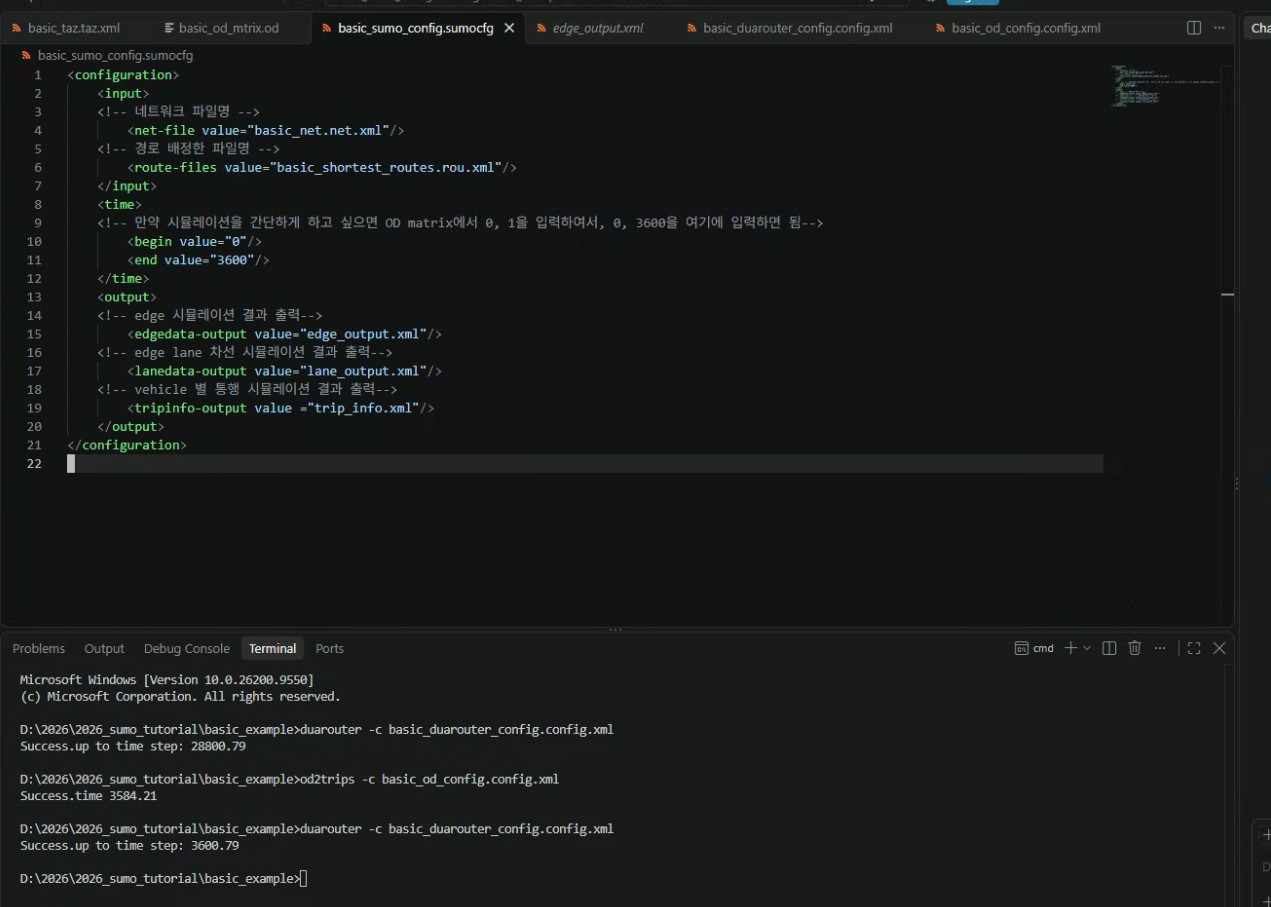
\includegraphics[keepaspectratio]{image/sumo_config.jpeg}}

\begin{enumerate}
\def\labelenumi{\arabic{enumi}.}
\setcounter{enumi}{2}
\item
  윈도우 파일 탐색기 켜기 \textgreater{} 프로젝트 폴더 \textgreater{}
  'basic\_sumo\_config.sumocfg'위에서 오른쪽 마우스키 클릭
  \textgreater{} sumo 열기 클릭
  \pandocbounded{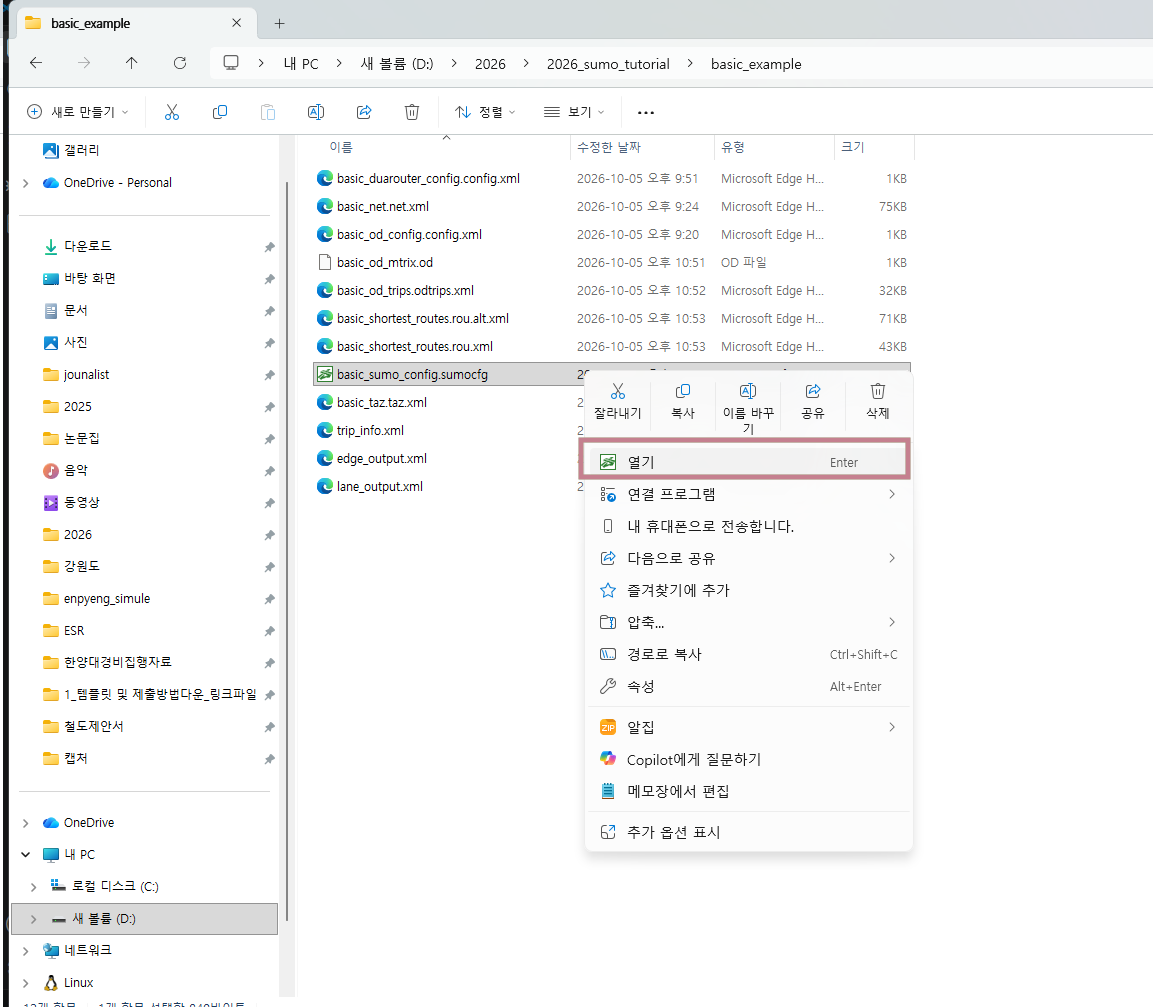
\includegraphics[keepaspectratio]{image/sumo_01.png}}
\item
  상단 도구줄에서 delay 200 입력, standard \textgreater{} real world로
  변경, 재생 버튼 클릭
  \pandocbounded{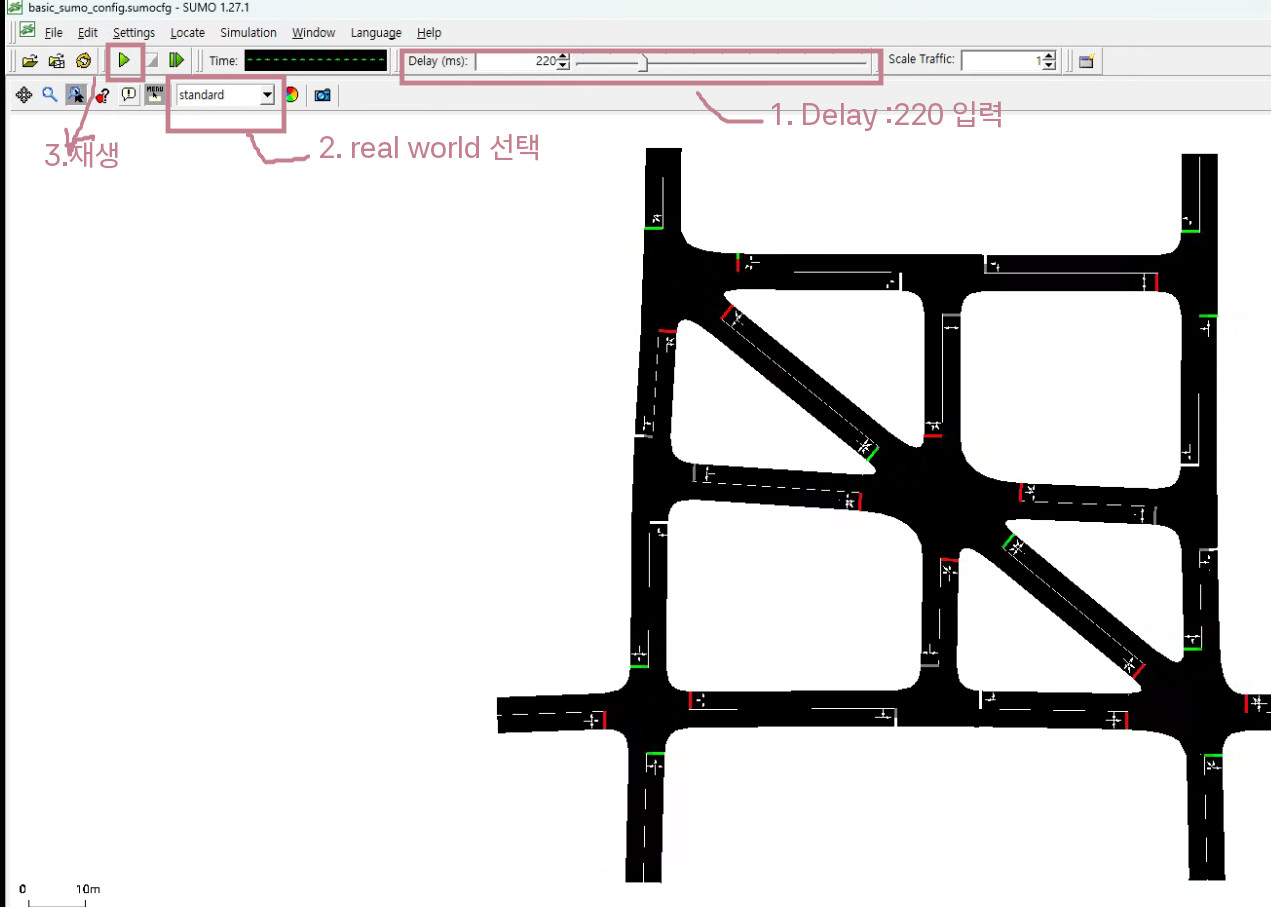
\includegraphics[keepaspectratio]{image/sumo2.jpeg}}
\end{enumerate}

시뮬레이션 영상
\pandocbounded{\includegraphics[keepaspectratio]{image/simule.gif}}

\begin{enumerate}
\def\labelenumi{\arabic{enumi}.}
\setcounter{enumi}{4}
\tightlist
\item
  3600초 동안의 시뮬레이션이 완료되고 나서, vs code에서 프로젝트 폴더를
  열어보면 output file이 만들어진 것을 확인할 수 있습니다.
  \pandocbounded{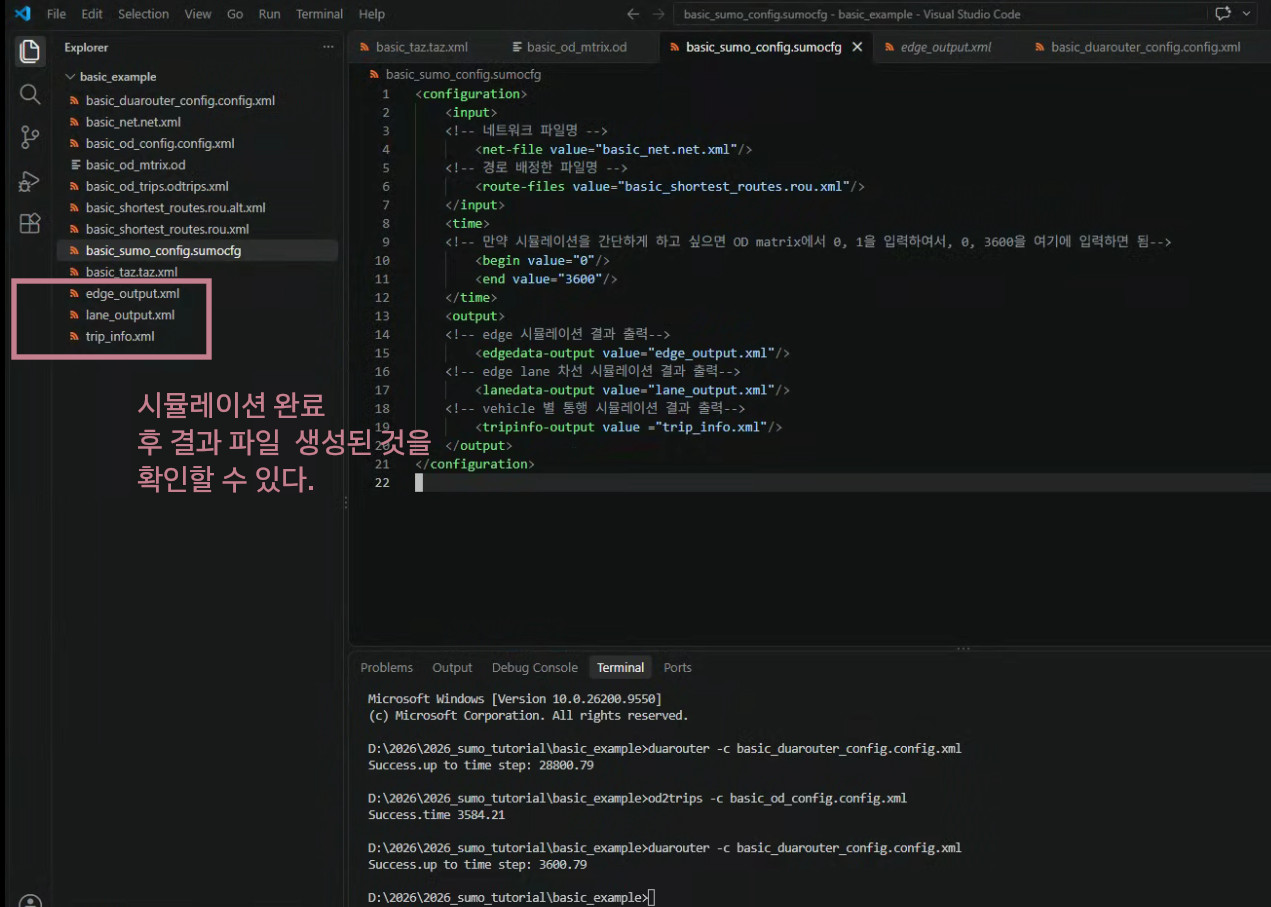
\includegraphics[keepaspectratio]{image/sumo_result.jpeg}}
\end{enumerate}

\chapter{결과 파일 해석}\label{uxacb0uxacfc-uxd30cuxc77c-uxd574uxc11d}

\section{edge\_output.xml Parameter
설명}\label{edge_output.xml-parameter-uxc124uxba85}

\begin{itemize}
\tightlist
\item
  travelTime : 평균 구간속도 기준 edge, lane 구간을 통과하는데 걸리는
  시간(초)
\item
  watingTime: lane에서 달리지 못하고 대기하는 자동차의 대기 시간의
  총합(대기시간)

  \begin{itemize}
  \tightlist
  \item
    ==watingTime이 직관적으로 이해하기 쉽다==
  \end{itemize}
\item
  timeLoss: desired 속도보다 느리게 달려서 잃게 되는 시간의 총합

  \begin{itemize}
  \tightlist
  \item
    desired의 결정방식
  \end{itemize}
\end{itemize}

\subsection{edge based}\label{edge-based}

{\def\LTcaptype{none} % do not increment counter
\begin{longtable}[]{@{}
  >{\raggedright\arraybackslash}p{(\linewidth - 4\tabcolsep) * \real{0.0471}}
  >{\raggedright\arraybackslash}p{(\linewidth - 4\tabcolsep) * \real{0.0554}}
  >{\raggedright\arraybackslash}p{(\linewidth - 4\tabcolsep) * \real{0.8975}}@{}}
\toprule\noalign{}
\begin{minipage}[b]{\linewidth}\raggedright
Name
\end{minipage} & \begin{minipage}[b]{\linewidth}\raggedright
Type
\end{minipage} & \begin{minipage}[b]{\linewidth}\raggedright
Description
\end{minipage} \\
\midrule\noalign{}
\endhead
\bottomrule\noalign{}
\endlastfoot
begin & (simulation) seconds & The first time step the values were
collected in \\
end & (simulation) seconds & The last time step + DELTA\_T in which the
reported values were collected \\
edge@id & (edge) id & The name of the reported edge \\
lane@id & (lane) id & The name of the reported lane \\
sampledSeconds & s & The number of vehicles that are present on the
edge/lane in each second summed up over the measurement interval (may be
subseconds if a vehicle enters/leaves the edge/lane). \\
traveltime & s & Time needed to pass the edge/lane, note that this is
just an estimation based on the mean speed, not the exact time the
vehicles needed. The value is based on the time needed for the front of
the vehicle to pass the edge. \\
overlapTraveltime & s & Time needed to pass the edge/lane completely,
note that this is just an estimation based on the mean speed, not the
exact time the vehicles needed. The value is based on the time any part
of the vehicle was the edge. \\
density & \#veh/km & Vehicle density on the edge \\
overlapDensity & \#veh/km & Vehicle density on the edge. This value
counts vehicles if any part along it's length touches the edge. This
should not be used for flow computation \\
laneDensity & \#veh/km/lane & Vehicle density on the edge per lane \\
occupancy & \% & Occupancy of the edge/lane in \%. A value of 100 would
indicate vehicles standing bumper to bumper on the whole edge
(minGap=0). \\
waitingTime & s & The total number of seconds vehicles were considered
halting (speed \textless{} speedThreshold). Summed up over all
vehicles \\
timeLoss & s & The total number of seconds vehicles lost due to driving
slower than desired (summed up over all vehicles) \\
speed & m/s & The mean speed on the edge/lane within the reported
interval. \textbf{Caution:} This is an average over time and space
(space-mean-speed), rather than a local average over the vehicles
(time-mean-speed). Since slow vehicles spend more time on the edge they
will have a proportionally bigger influence on average speed. \\
speedRelative & - & quotient of mean speed value (see above) and the
lane speed limit \\
departed & \#veh & The number of vehicles that have been emitted onto
the edge/lane within the described interval \\
arrived & \#veh & The number of vehicles that have finished their route
on the edge lane \\
entered & \#veh & The number of vehicles that have entered the edge/lane
by moving from upstream \\
left & \#veh & The number of vehicles that have left the edge/lane by
moving downstream \\
laneChangedFrom & \#veh & The number of vehicles that changed away from
this lane \\
laneChangedTo & \#veh & The number of vehicles that changed to this
lane \\
vaporized & \#veh & The number of vehicles vaporized on this edge
\textbf{(only present if \#veh \textgreater{} 0)} \\
teleported & \#veh & The number of vehicles teleported from this edge
\textbf{(only present if \#veh \textgreater{} 0)} \\
flow & \#veh/hour & The number of vehicles passing this edge per hour.
Vehicles that depart on this edge beyond position 0 or arrive before the
end of the edge are fractionally disocunted \\
\end{longtable}
}

{\def\LTcaptype{none} % do not increment counter
\begin{longtable}[]{@{}
  >{\raggedright\arraybackslash}p{(\linewidth - 4\tabcolsep) * \real{0.0483}}
  >{\raggedright\arraybackslash}p{(\linewidth - 4\tabcolsep) * \real{0.1018}}
  >{\raggedright\arraybackslash}p{(\linewidth - 4\tabcolsep) * \real{0.8499}}@{}}
\toprule\noalign{}
\begin{minipage}[b]{\linewidth}\raggedright
Attribute Name
\end{minipage} & \begin{minipage}[b]{\linewidth}\raggedright
Value Type
\end{minipage} & \begin{minipage}[b]{\linewidth}\raggedright
Description
\end{minipage} \\
\midrule\noalign{}
\endhead
\bottomrule\noalign{}
\endlastfoot
\textbf{id} & id (string) & The id of this set of measurements. This
user-defined id is needed for differentiating between multiple sets of
measurements in a single output file. \\
\textbf{file} & filename & The path to the output file. The path may be
relative. \\
period (alias freq) & int (time) & The aggregation period the values the
detector collects shall be summed up. If not given the whole time
interval from begin to end (see below) is aggregated. \\
begin & int (time) & The time to start writing (intervals starting
before this time are discarded). If not given, the simulation's begin is
used. \\
end & int (time) & The time to end writing (intervals starting at or
after this time are discarded). If not given the simulation's end is
used. \\
excludeEmpty & string (true, false, defaults, modified) & If set to
true, edges/lanes which were not used by a vehicle during this period
will not be written; \emph{default: false}. If set to ``defaults''
default values for travel time and speed depending on edge length and
maximum speed get printed, ``modified'' will print values only for empty
edges which have a dynamically adapted maximum speed. \\
withInternal & bool & If set, junction internal edges/lanes will be
written as well; \emph{default: false}. \\
maxTraveltime & float (time) & The maximum traveltime in seconds to
write if only very small movements occur; \emph{default 100000}. \\
minSamples & float (time) & The minimum total number of seconds vehicles
have to be on the edge / lane to consider it non-empty; \emph{default:
\textgreater0}. \\
speedThreshold & float (m/s) & The maximum speed to consider a vehicle
halting; \emph{default 0.1}. \\
vTypes & string & space separated list of vehicle type ids to consider.
If not given, all vTypes will be considered. \\
trackVehicles & bool & whether aggregation should be performed over all
vehicles that entered the edge/lane in the aggregation interval \\
detectPersons & string list & whether pedestrians shall be recorded
instead of vehicles. Allowed value is \emph{walk}. \textbf{Note:}
further modes are planned \\
writeAttributes & string list & list of attribute names that shall be
written (defaults to all attribute) \\
edges & string list & restrict output to the given list of edge ids \\
edgesFile & filename & restrict output to the given the list of edges
given in file (either one edgeID per line or an id prefixed with `edge:'
as in a
\href{https://sumo.dlr.de/docs/Netedit/editModesCommon.html\#selection_operations}{selection
file}) \\
\end{longtable}
}

\chapter{Reference}\label{reference}

\begin{itemize}
\tightlist
\item
  \href{https://sumo.dlr.de/docs/Simulation/Output/Lane-_or_Edge-based_Traffic_Measures.html}{sumo
  document : Lane or Edge based traffic measures}
\item
  \href{https://sumo.dlr.de/docs/Simulation/Output/TripInfo.html}{sumo
  document : trip info}
\end{itemize}

\bookmarksetup{startatroot}

\chapter{OSM Network import}\label{osm-network-import}

\begin{enumerate}
\def\labelenumi{\arabic{enumi}.}
\item
  \href{https://www.openstreetmap.org/}{OpenStreetMap} 접속
\item
  대상지 찾기
\item
  좌측상단 \texttt{내보내기} 클릭
\item
  \texttt{수동으로\ 다른\ 지역\ 선택} 클릭
\item
  대상지 범위만큼 조절하고 \texttt{내보내기} 클릭
  \pandocbounded{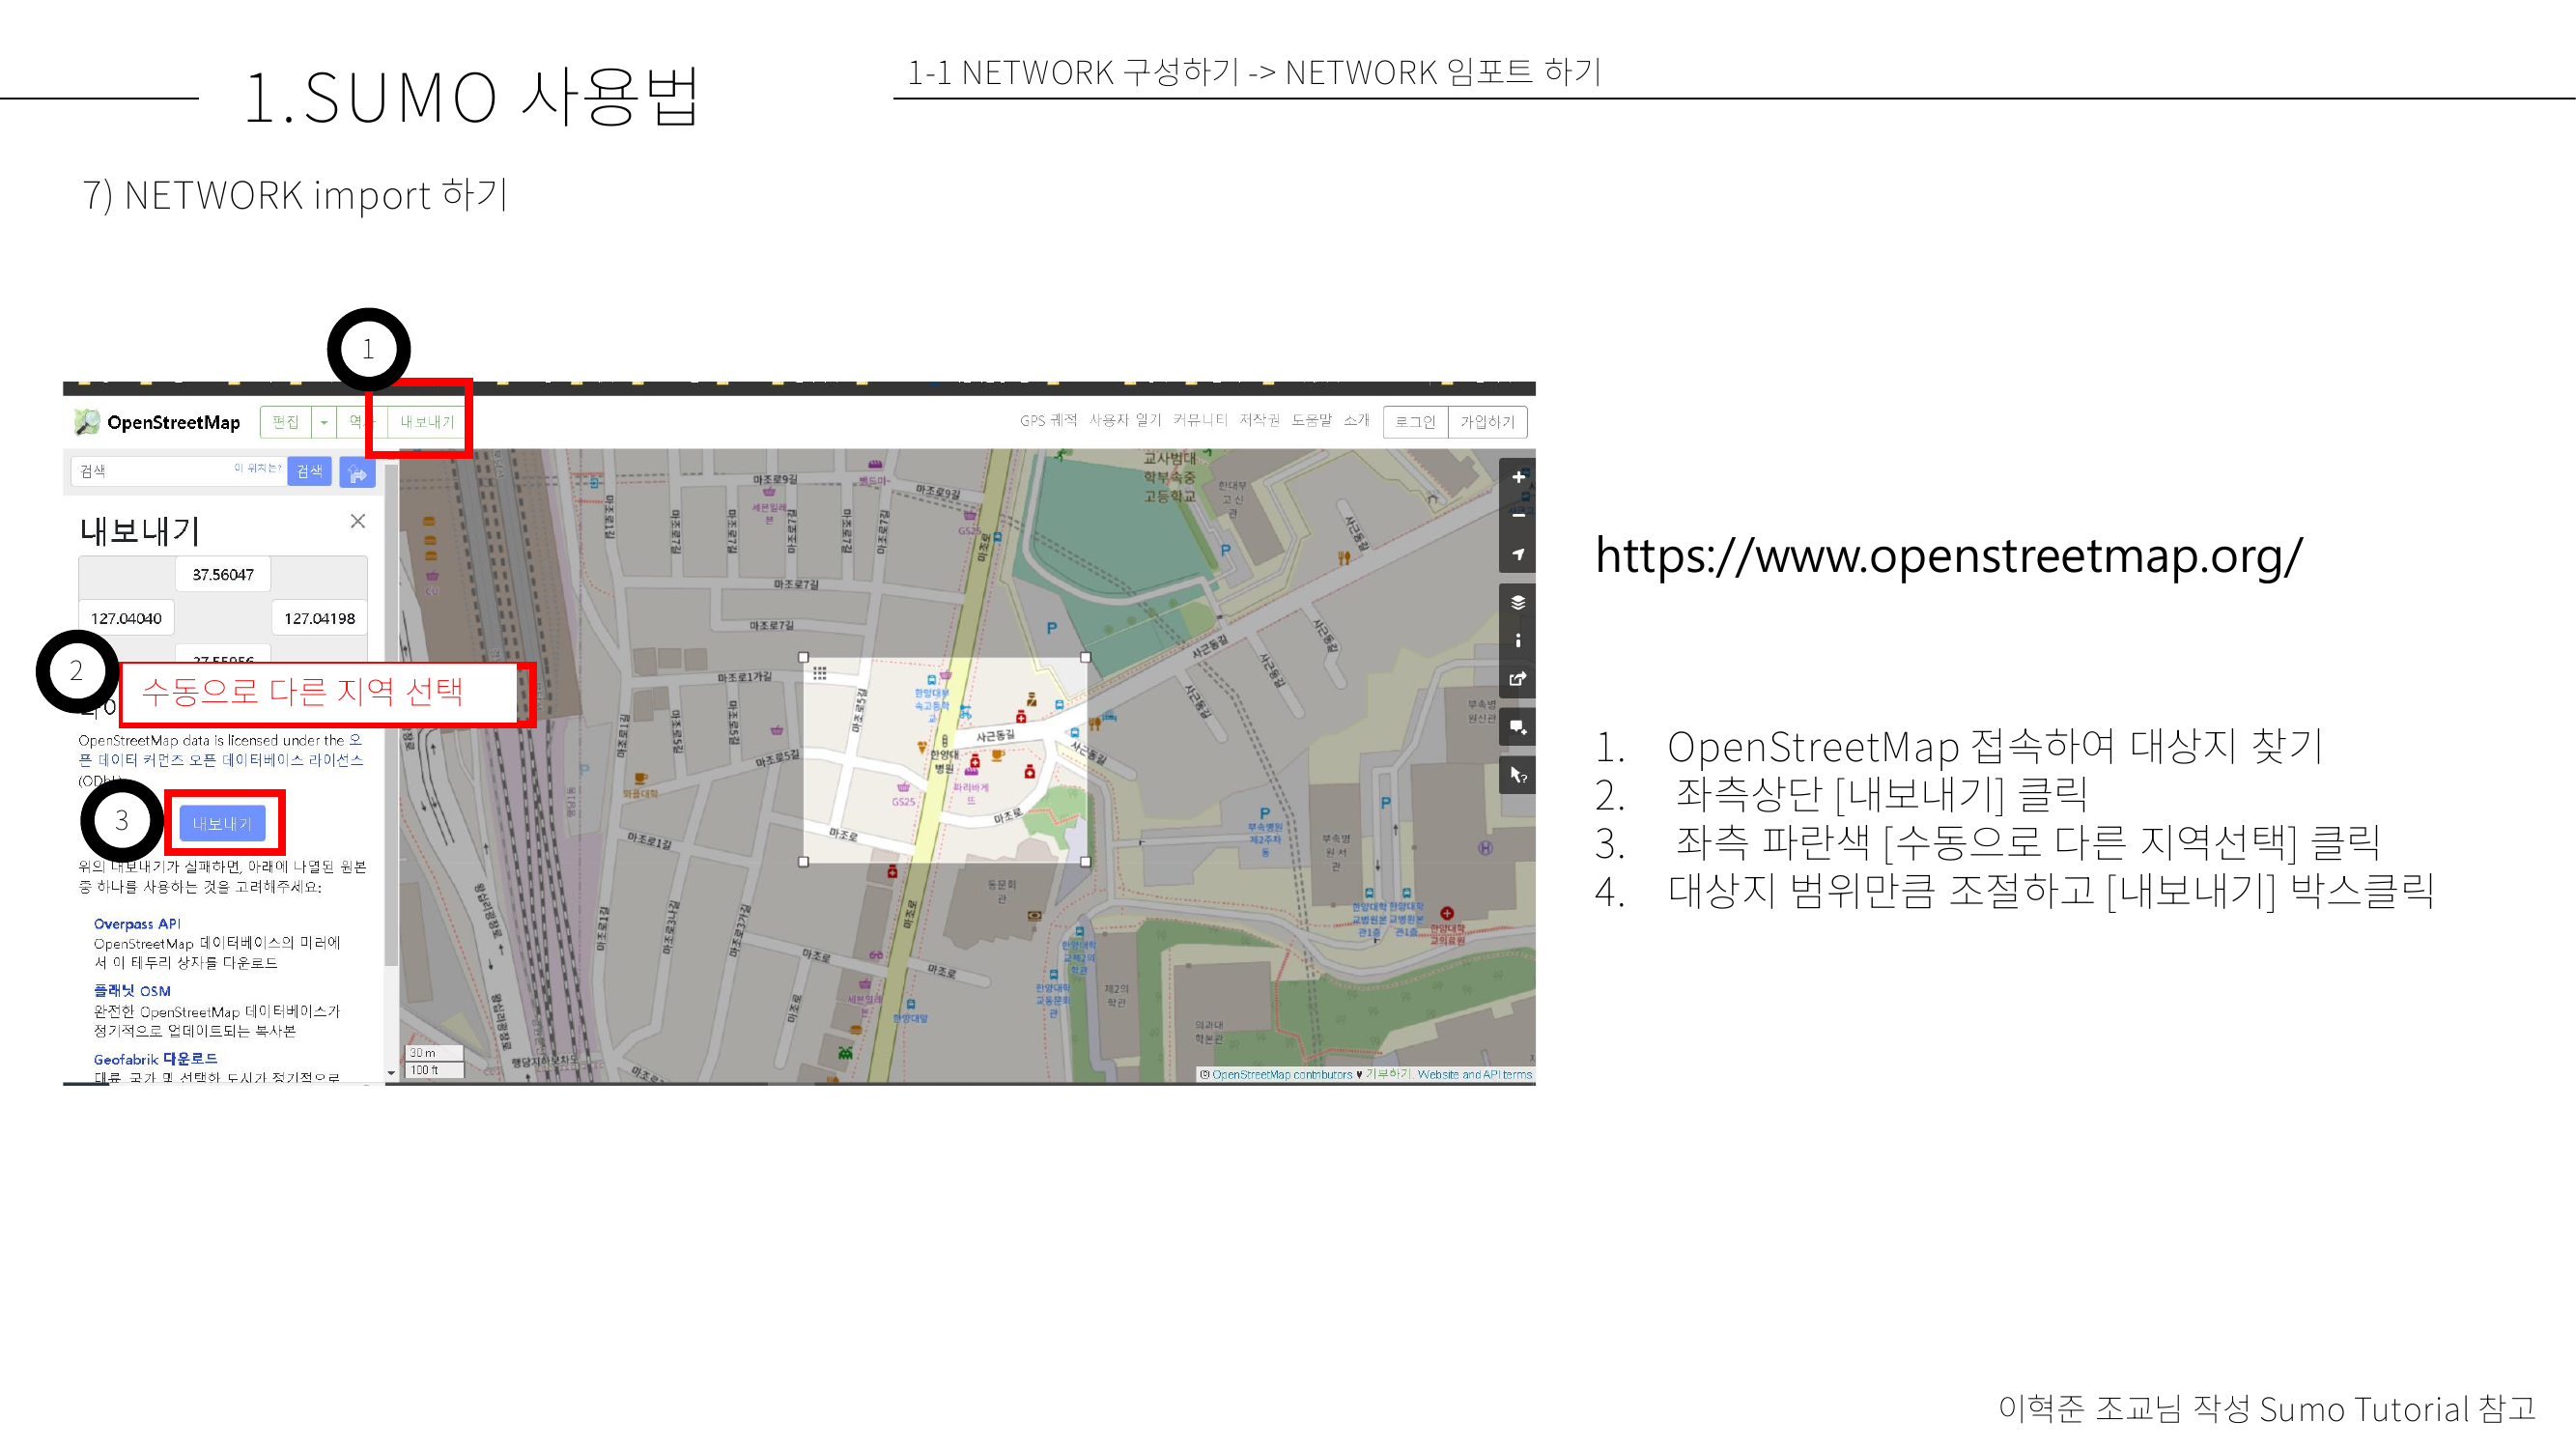
\includegraphics[keepaspectratio]{image/page-19.png}}
\item
  osm\_용 별도 프로젝트 폴더 만들기 \texttt{oms\_sumo}와 같이 생성
\item
  다운로드 받은 map.osm을 해당 프로젝트 폴더로 옮기기
  \pandocbounded{\includegraphics[keepaspectratio]{image/page-20.pdf}}
\item
  \texttt{Net\ Edit} 실행하여
  \texttt{File\textgreater{}Import\ Foreign\ Network}클릭
\item
  다운로드 받은 \texttt{map.osm} 선택
\item
  좌측 하단 확인 클릭
  \pandocbounded{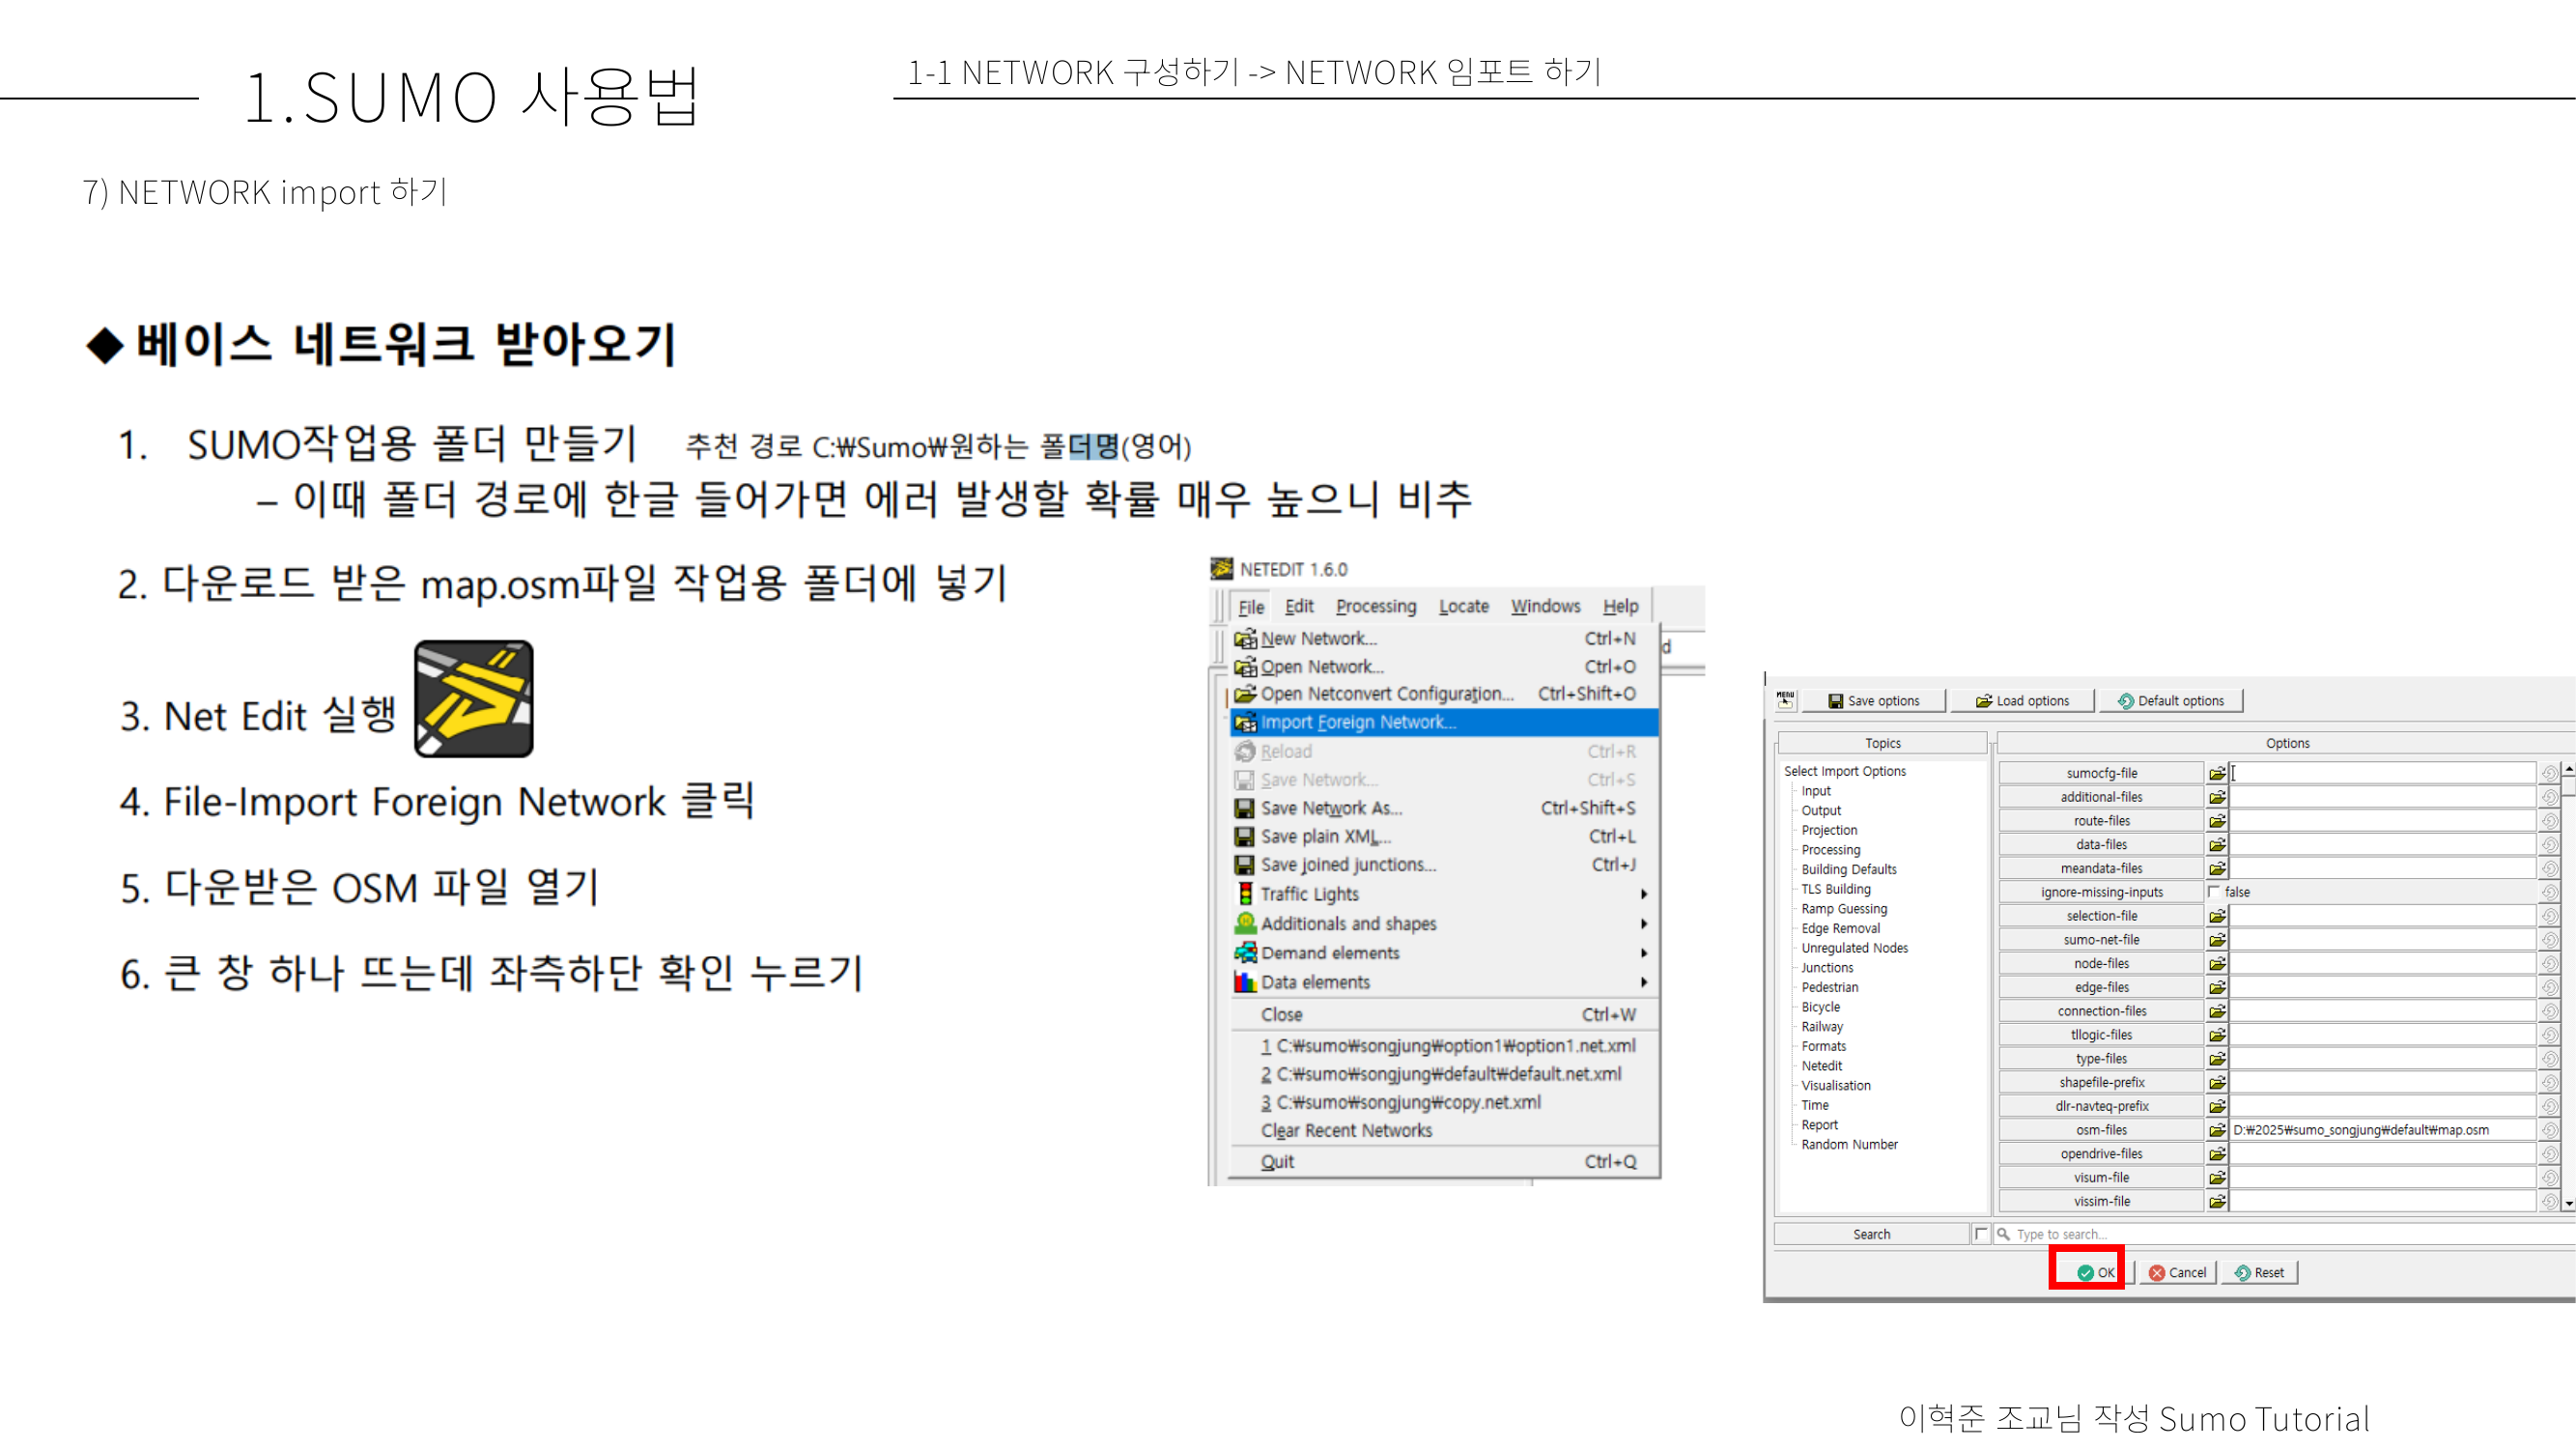
\includegraphics[keepaspectratio]{image/page-21.png}}
\end{enumerate}

\bookmarksetup{startatroot}

\chapter{요약}\label{uxc694uxc57d}

\section{SUMO 사용 순서}\label{sumo-uxc0acuxc6a9-uxc21cuxc11c}

\begin{enumerate}
\def\labelenumi{\arabic{enumi}.}
\tightlist
\item
  교통 공급(Supply) 정의 교통 인프라 공급을 정의하는 것
\end{enumerate}

\begin{itemize}
\tightlist
\item
  Network 파일 만들기

  \begin{itemize}
  \tightlist
  \item
    도로 Edge 속성 설정

    \begin{itemize}
    \tightlist
    \item
      차선 수
    \item
      허용 교통 수단
    \item
      최고 속도 등
    \end{itemize}
  \item
    교차로 설정
  \item
    신호 설정 등
  \end{itemize}
\end{itemize}

\begin{enumerate}
\def\labelenumi{\arabic{enumi}.}
\setcounter{enumi}{1}
\tightlist
\item
  교통 수요(Demand) 정의 교통 수요를 정의하는 것, TAZ와 OD 기반으로
  정의할 수 있다.
\end{enumerate}

\begin{itemize}
\tightlist
\item
  TAZ 파일 작성

  \begin{itemize}
  \tightlist
  \item
    TAZ에 속한 edge 작성, sink, source 구분
  \end{itemize}
\item
  OD matrix 작성

  \begin{itemize}
  \tightlist
  \item
    TAZ를 단위로 od matrix 작성
  \item
    시작시각, 종료시각 입력
  \end{itemize}
\item
  od2trips로 OD matrix에 따른 통행 생성

  \begin{itemize}
  \tightlist
  \item
    od2trips config 파일\\
  \end{itemize}
\item
  duarouter로 통행에 경로 배정

  \begin{itemize}
  \tightlist
  \item
    duarouter config 파일
  \end{itemize}
\end{itemize}

\begin{enumerate}
\def\labelenumi{\arabic{enumi}.}
\setcounter{enumi}{2}
\tightlist
\item
  시뮬레이션 sumo 실행
\end{enumerate}

\begin{itemize}
\tightlist
\item
  sumo config 파일 작성
\item
  시뮬레이션 실행
\item
  결과 파일 확인
\end{itemize}

\section{요약}\label{uxc694uxc57d-1}

하기 그림에 나타난 duarcfg\_file은 기초 실습의 duarouter config
파일이며, od2trips.config 또한 기초 실습의 od2trip의 config 파일입니다.
additional.xml은 금번 기초실습에서 sumo config파일에 합쳐서
서술하였습니다.

\pandocbounded{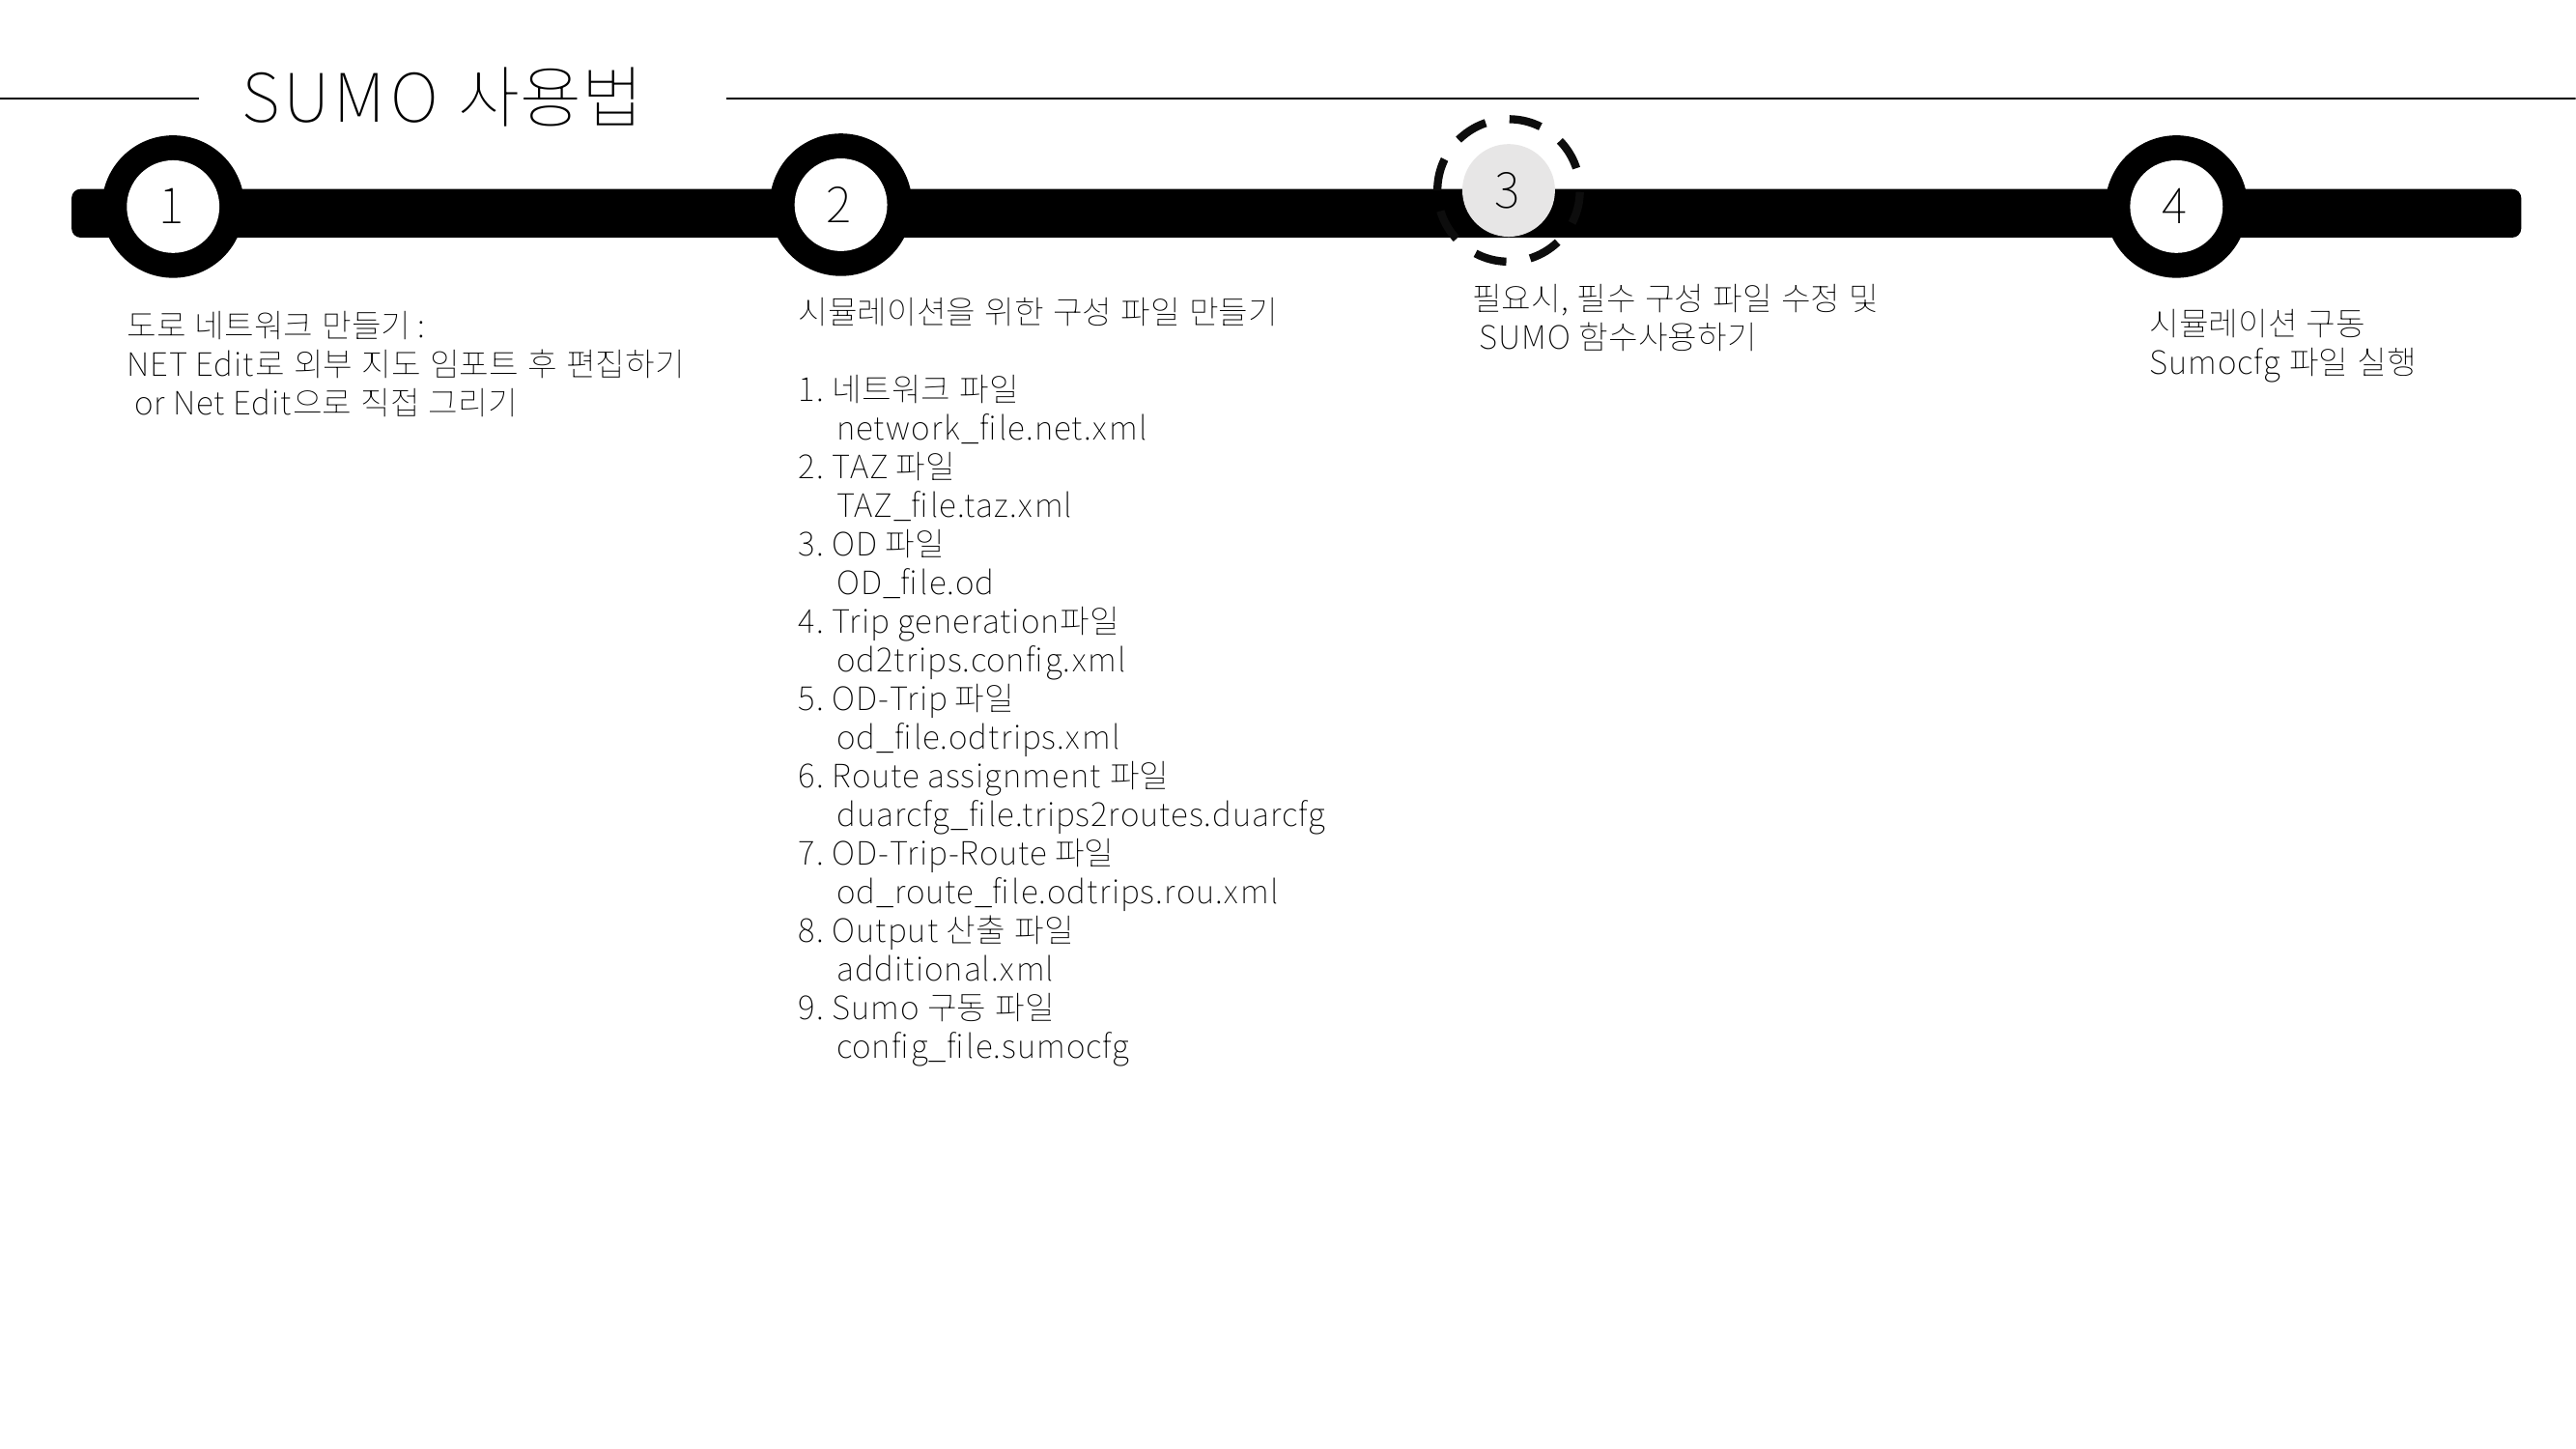
\includegraphics[keepaspectratio]{image/page-11.png}}
\pandocbounded{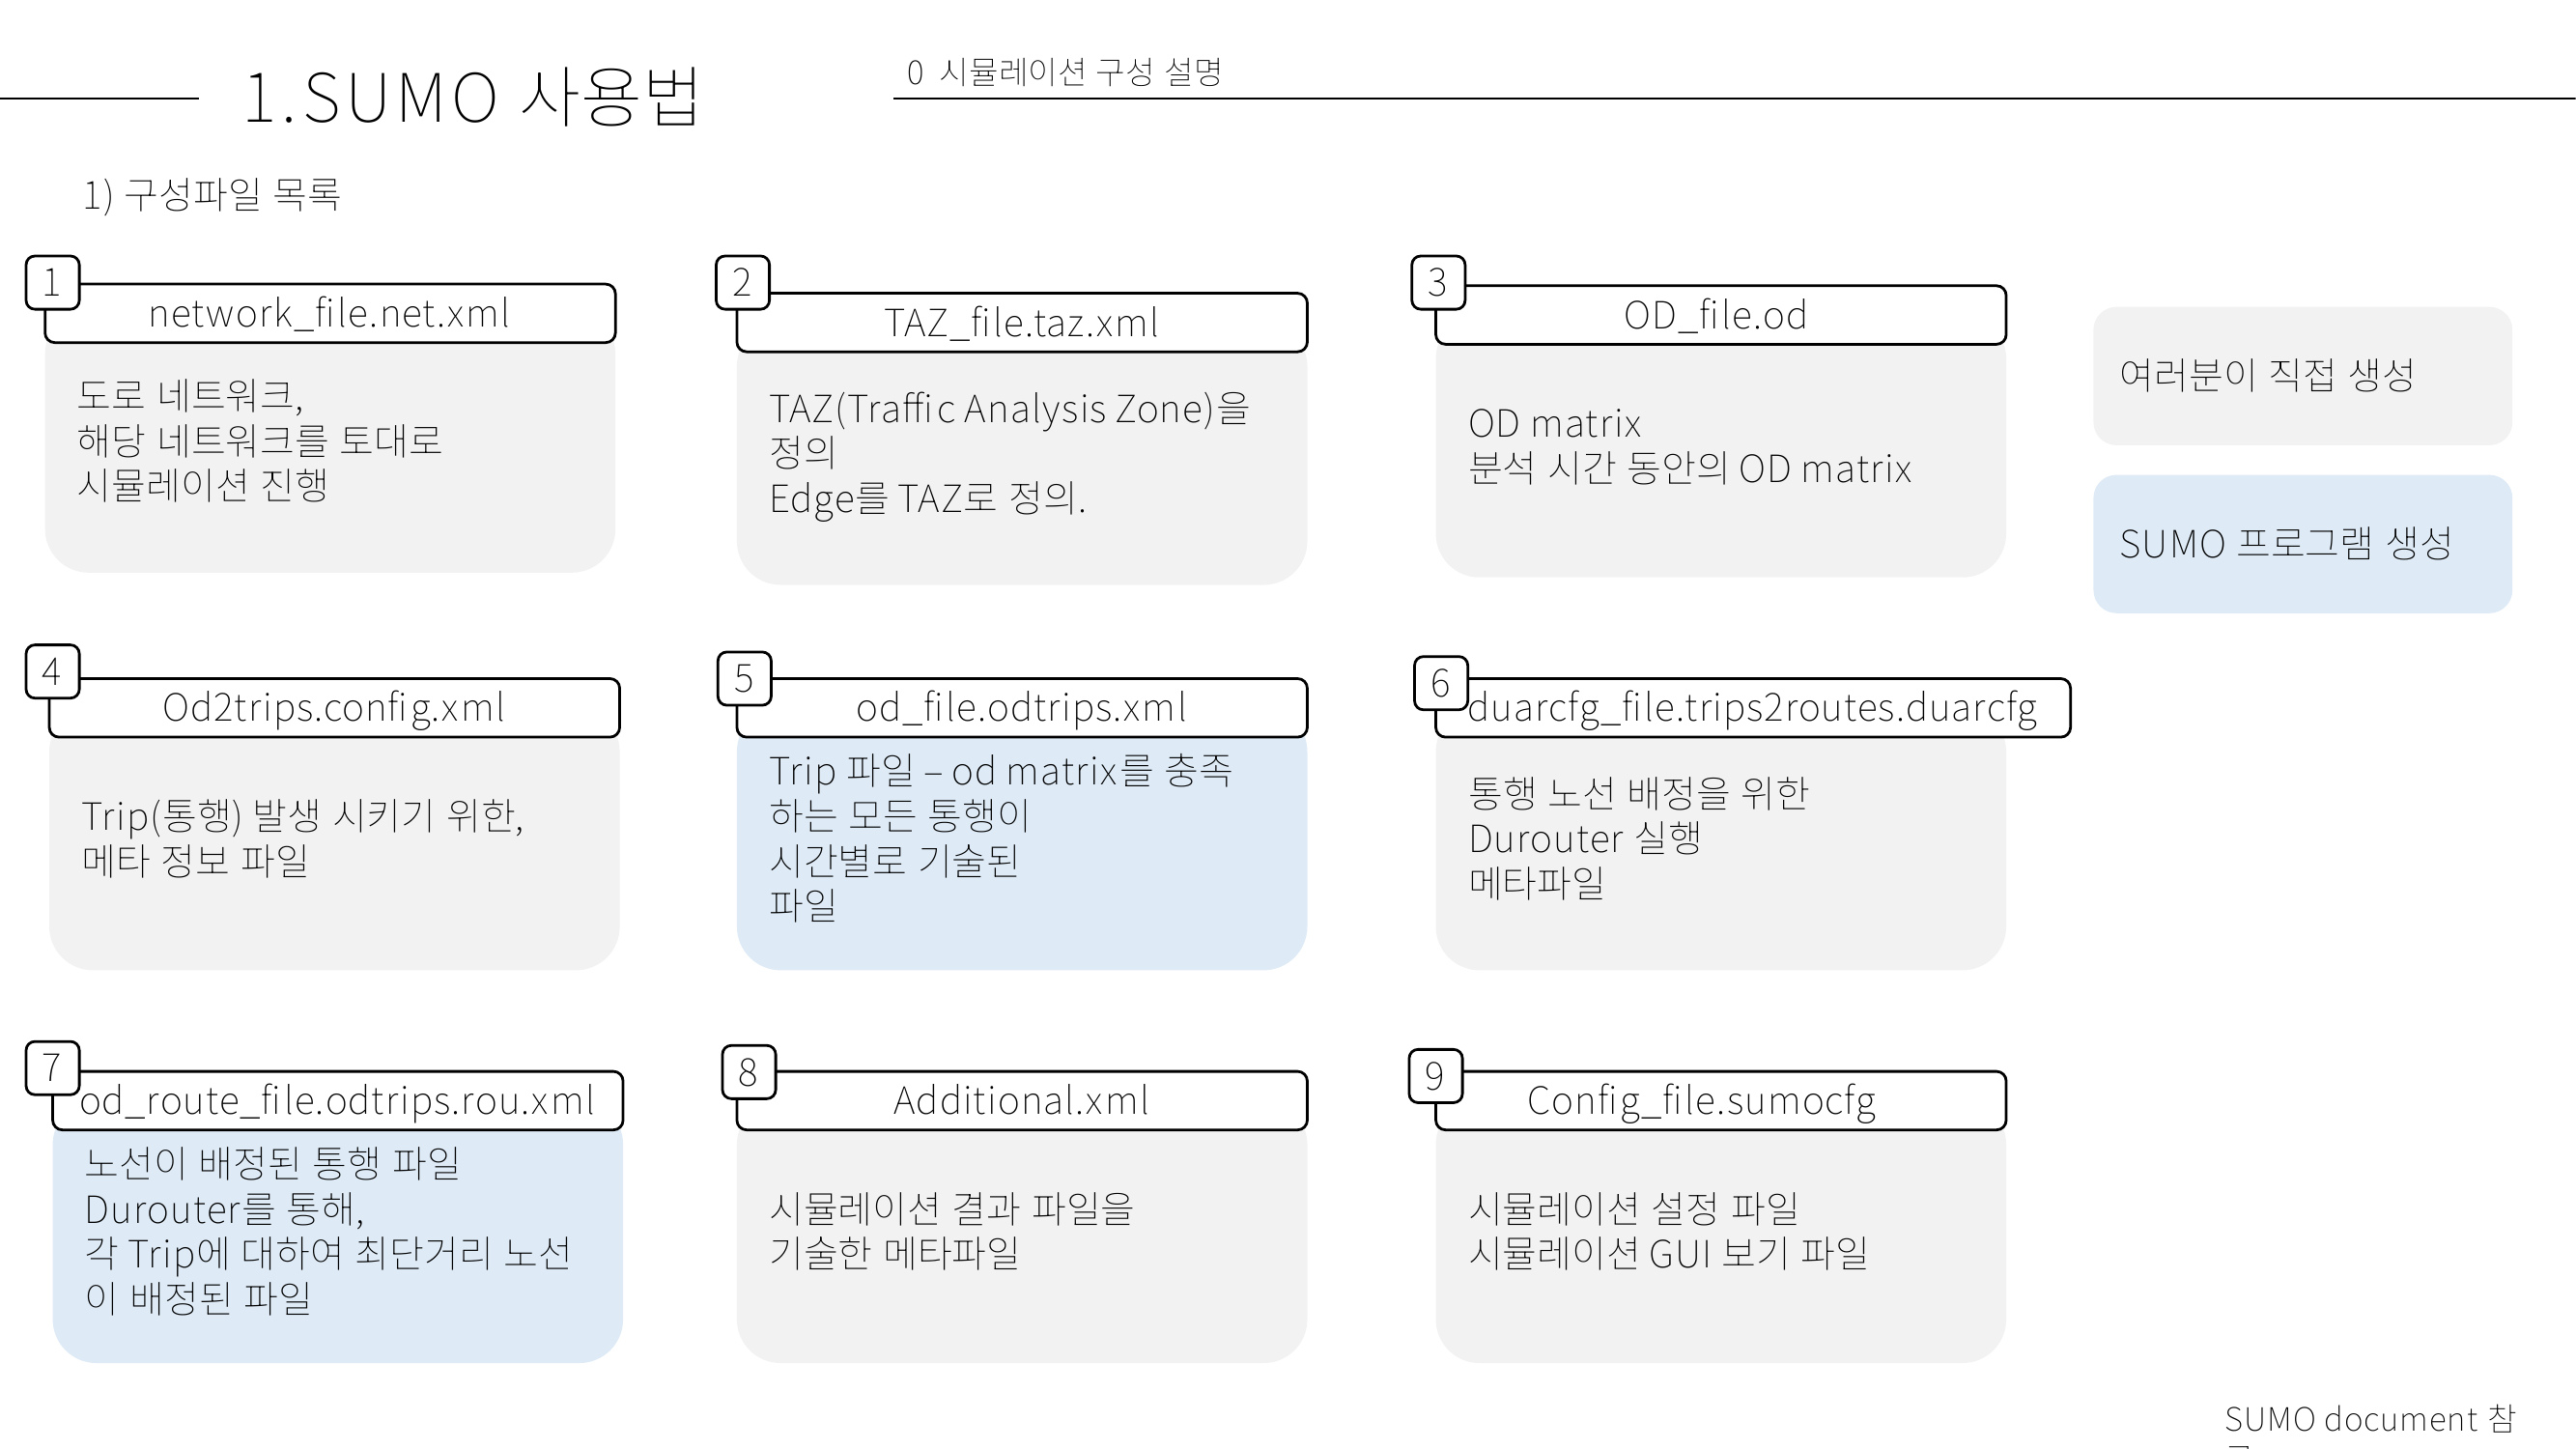
\includegraphics[keepaspectratio]{image/page-12.png}}
\pandocbounded{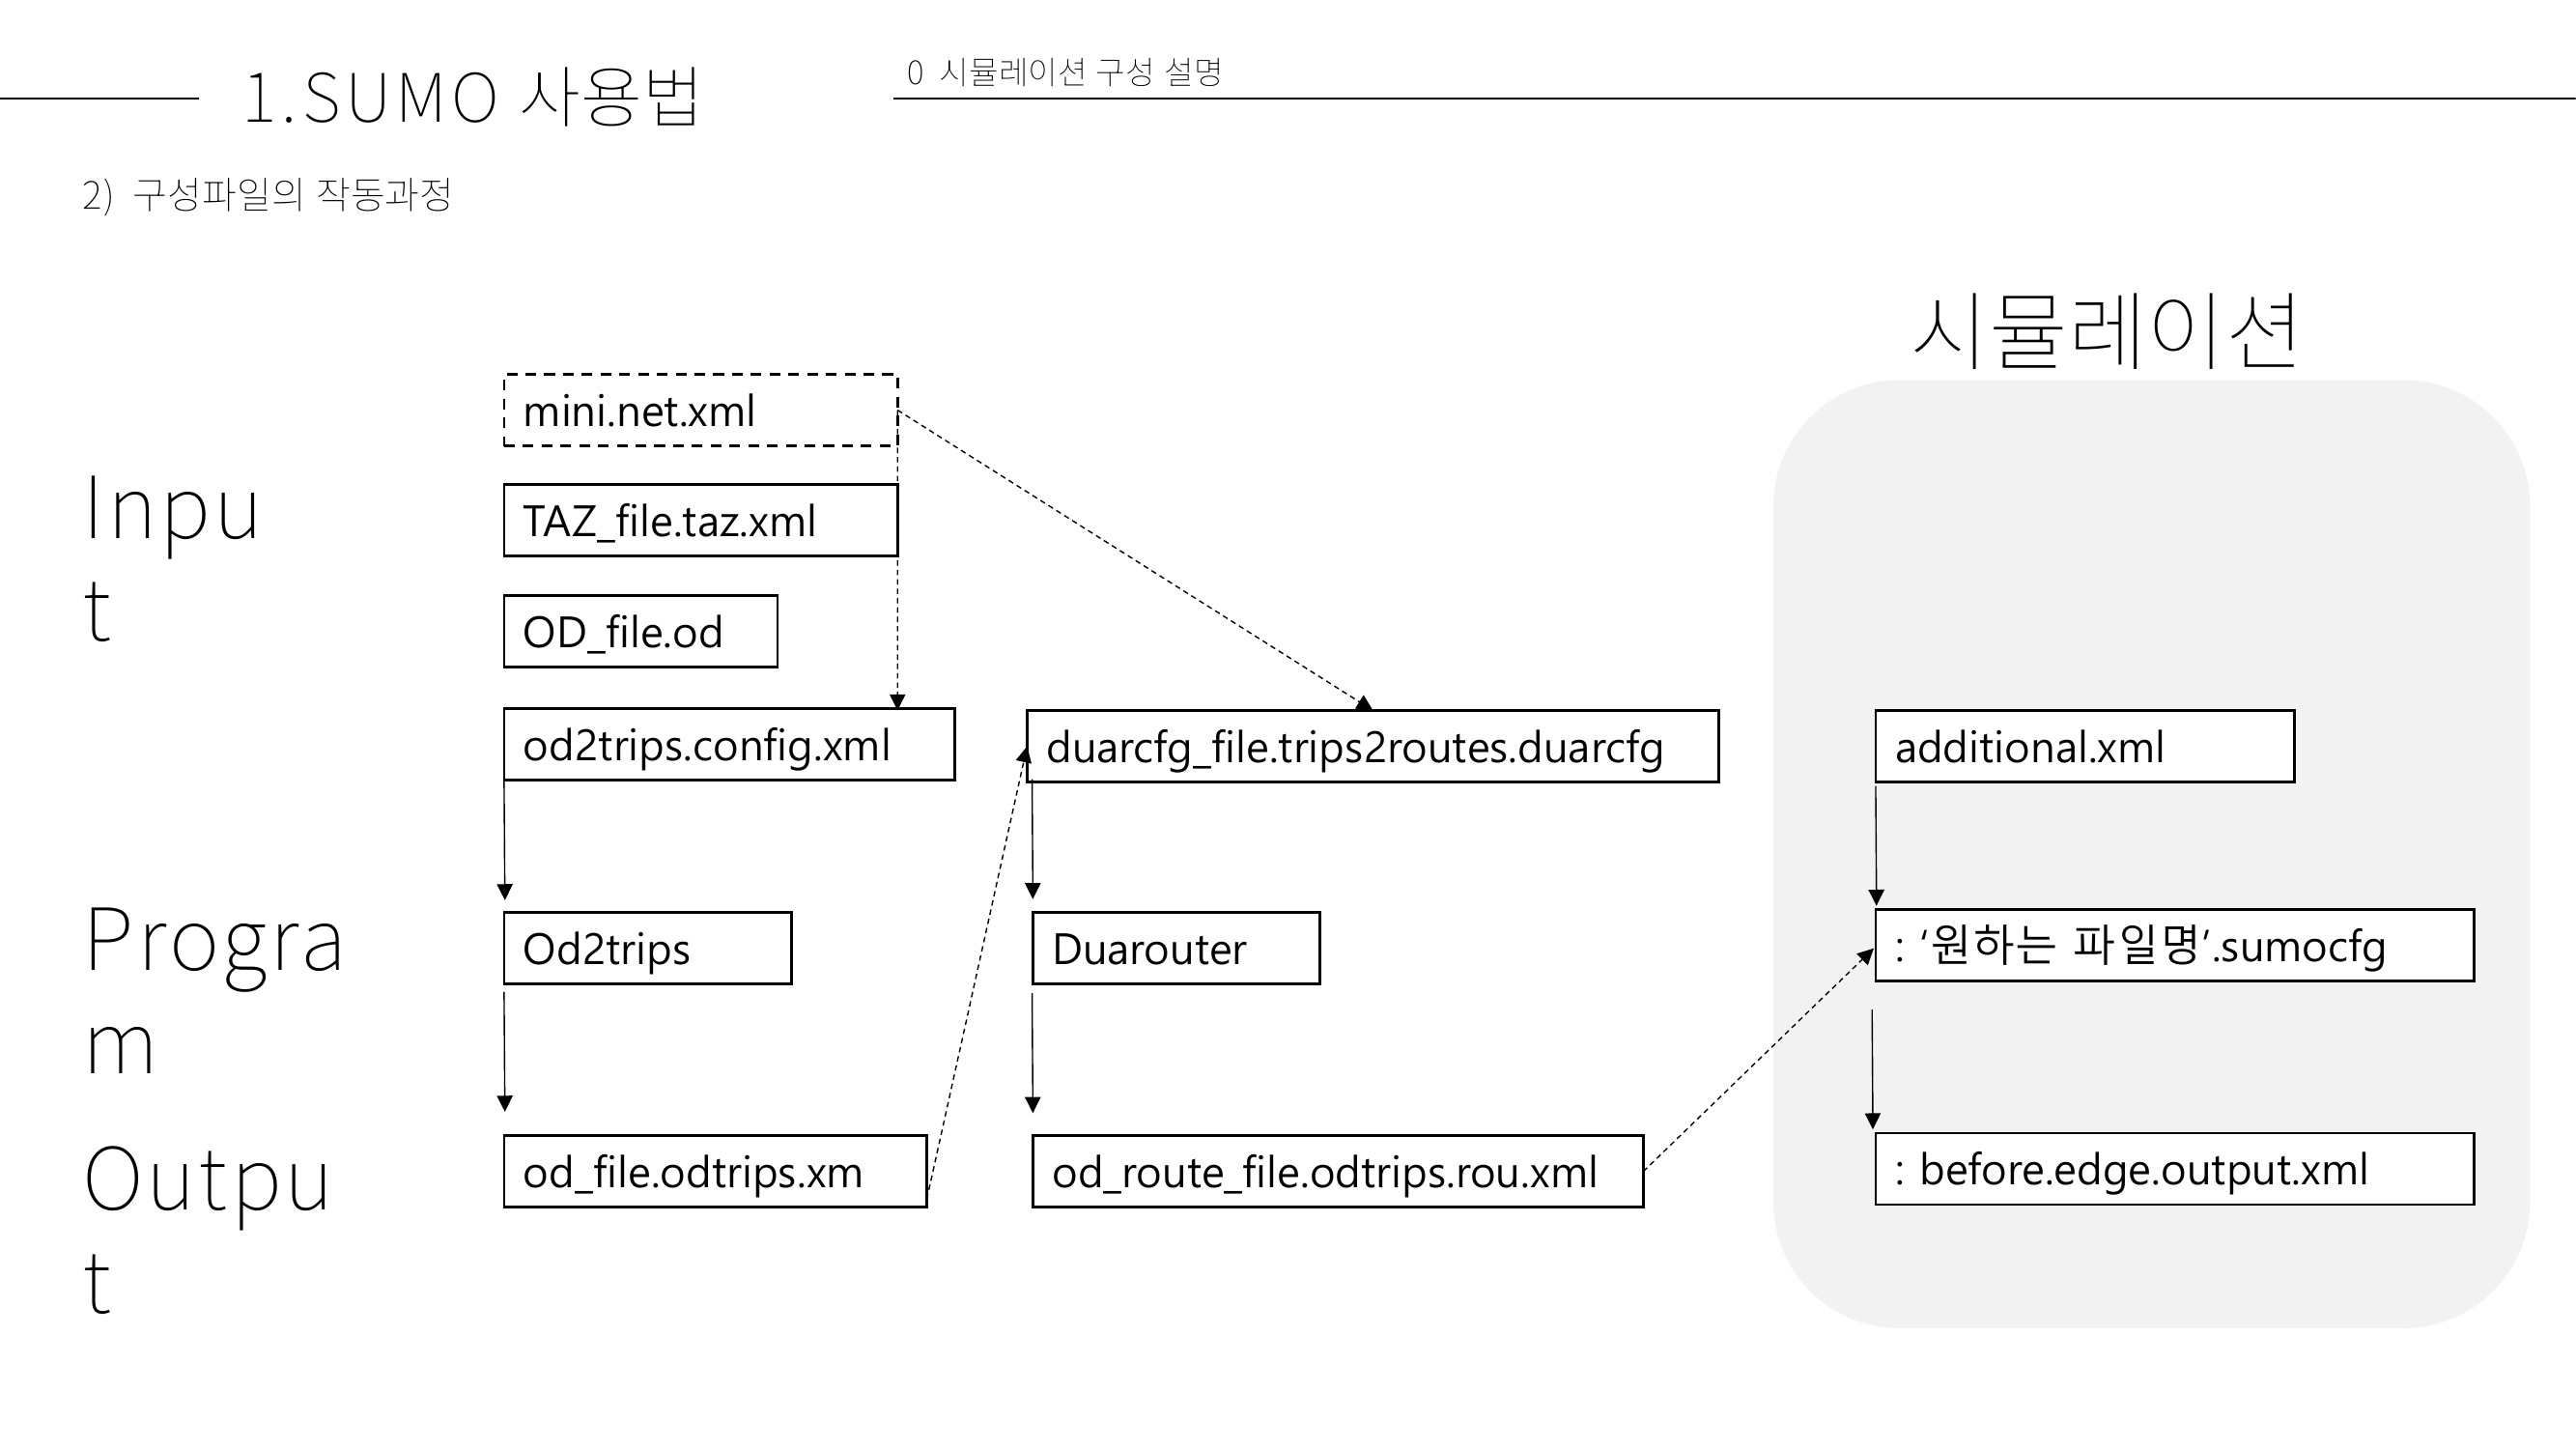
\includegraphics[keepaspectratio]{image/page-13.png}}

\bookmarksetup{startatroot}

\chapter{많이 묻는 질문}\label{uxb9ceuxc774-uxbb3buxb294-uxc9c8uxbb38}

\section{커넥션 버튼}\label{uxcee4uxb125uxc158-uxbc84uxd2bc}

편집 후 도로의 경우 Edge 사이에 흰 색 공백도 보여 도로가 제대로 연결되어
있는 것인지도 의아합니다.

\pandocbounded{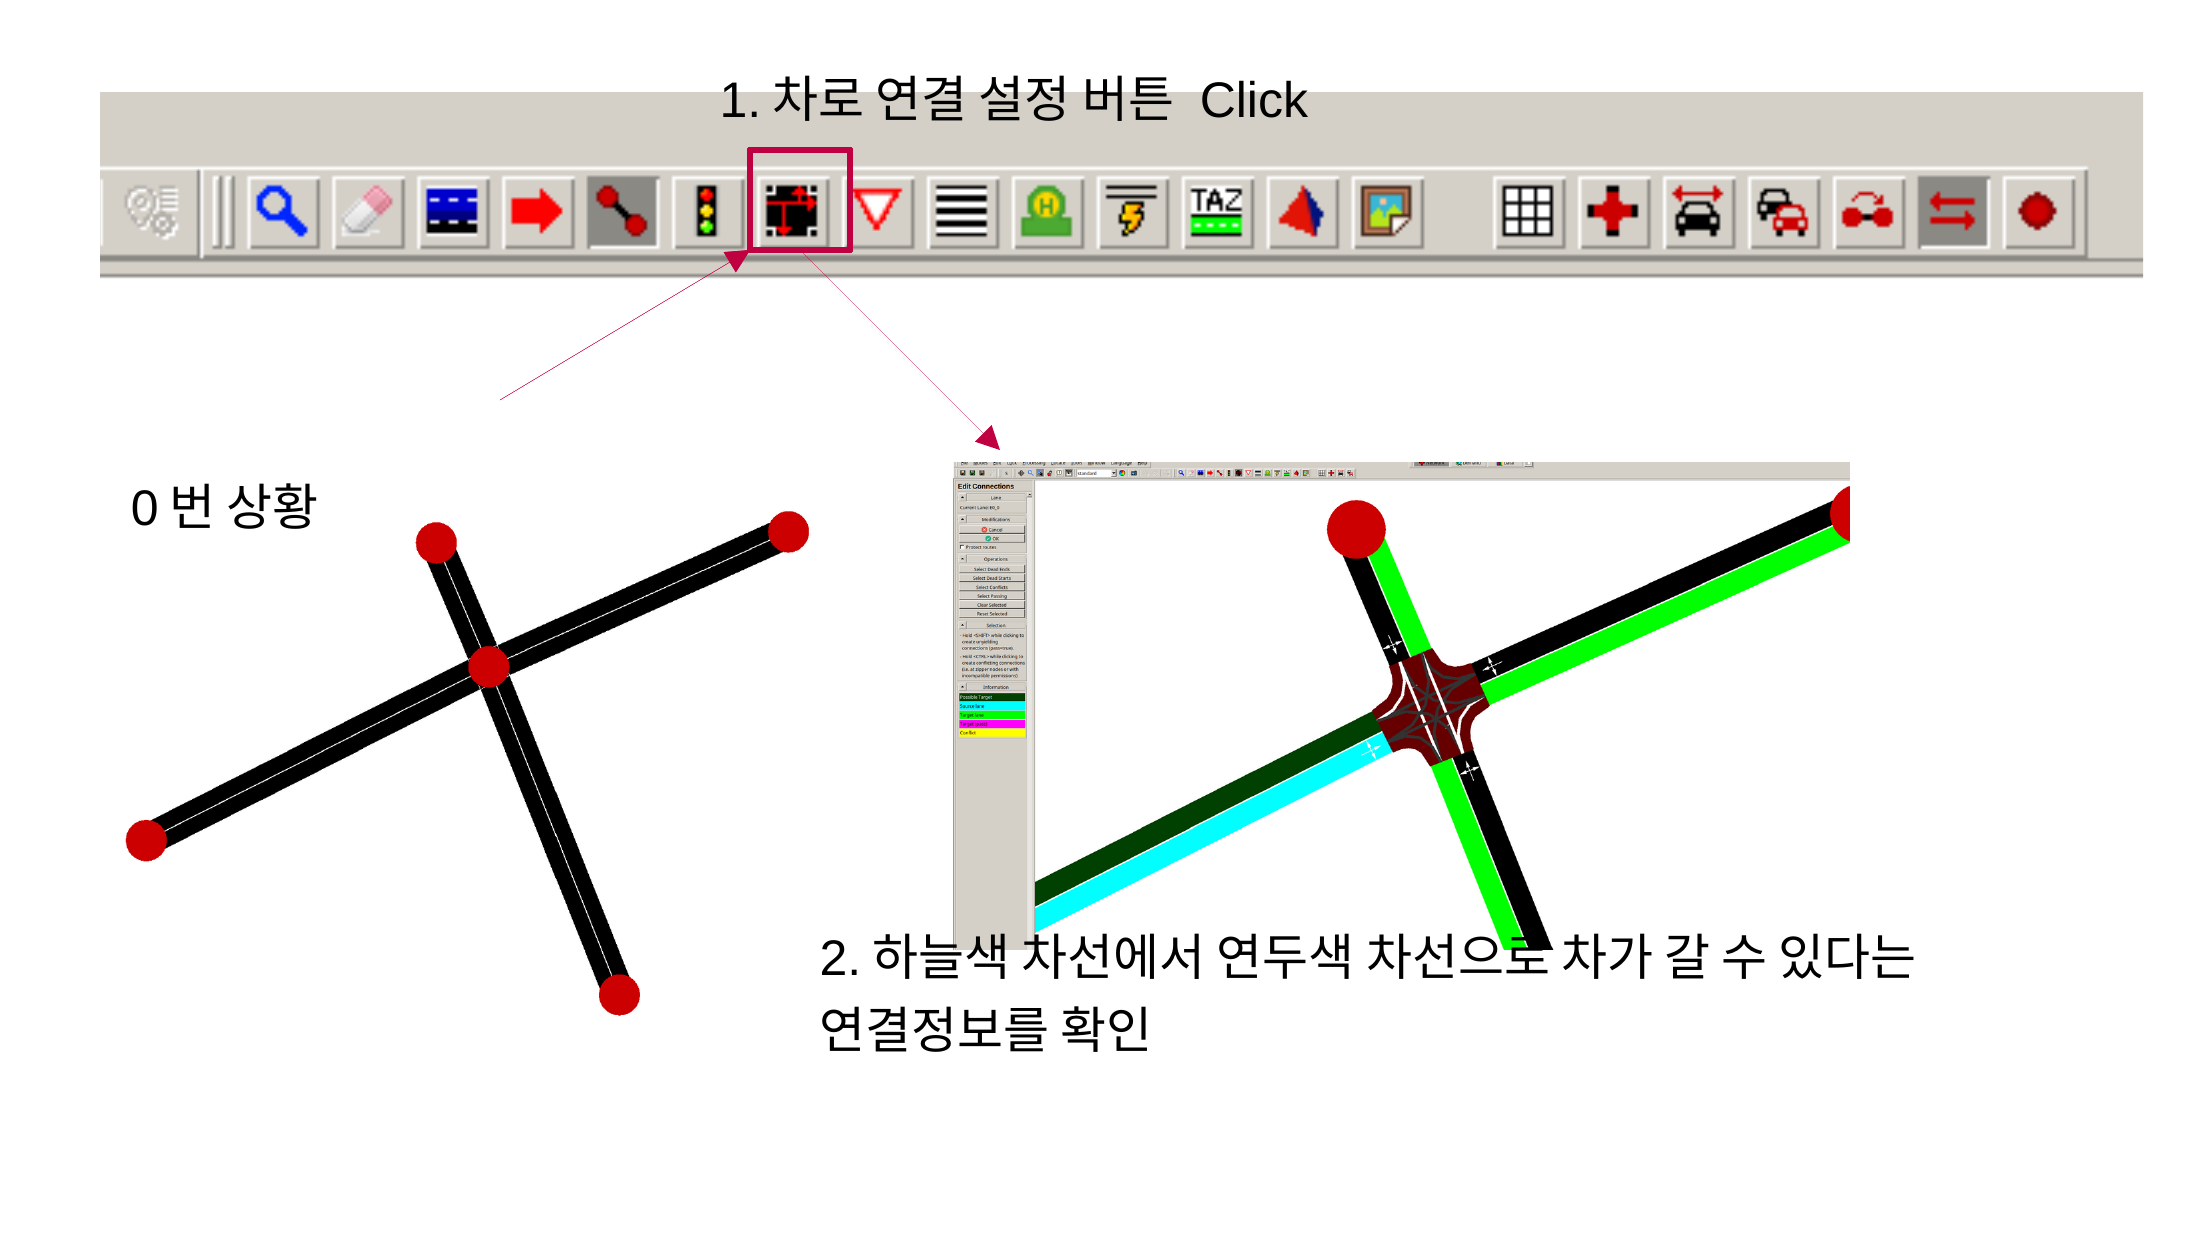
\includegraphics[keepaspectratio]{image/page-1.png}}
\pandocbounded{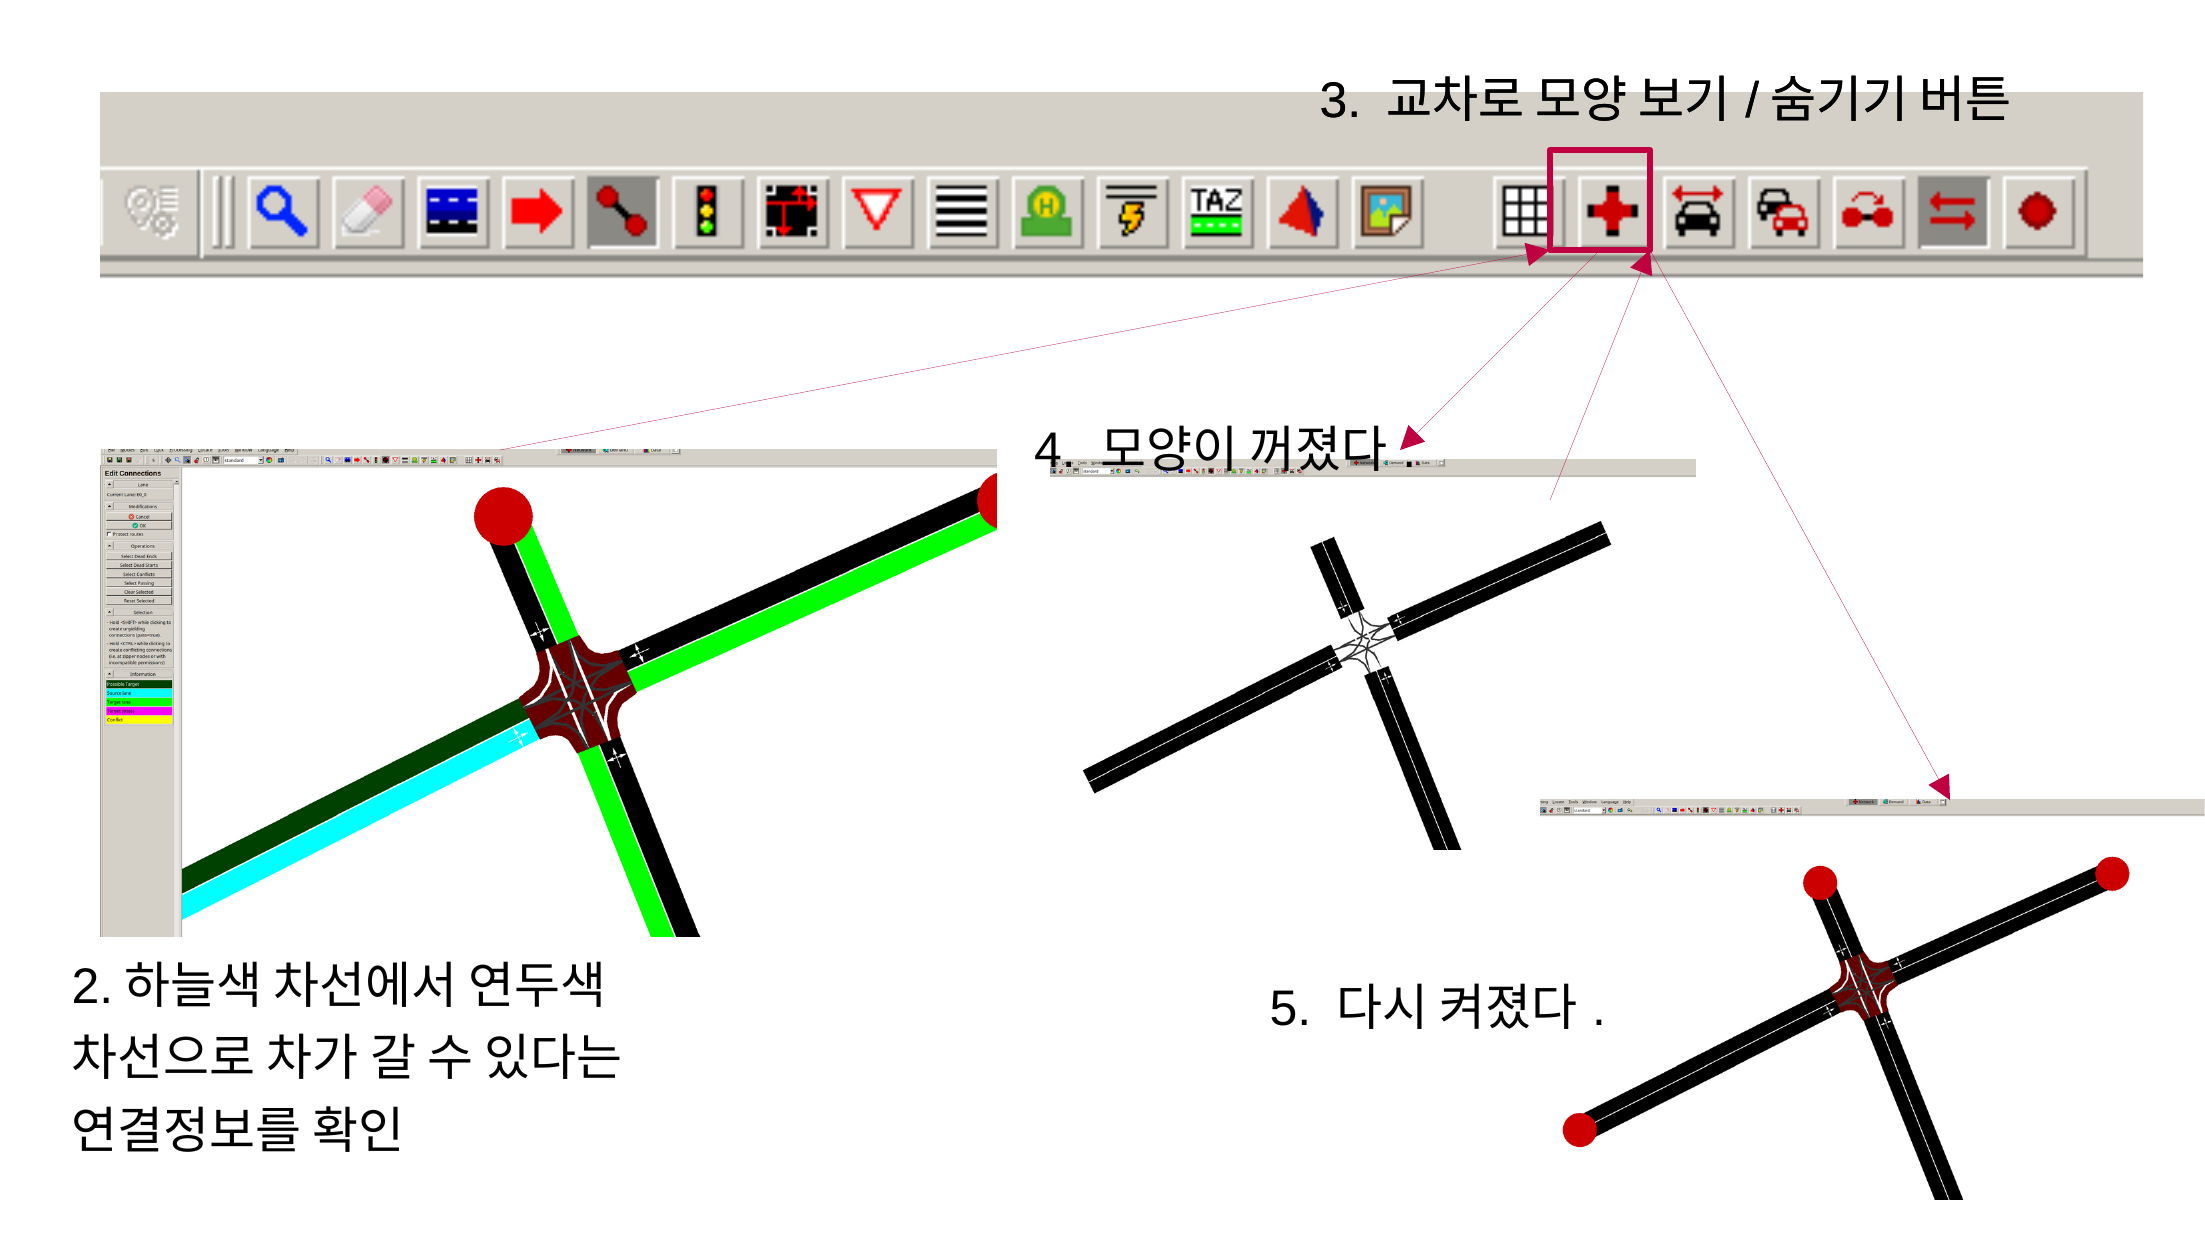
\includegraphics[keepaspectratio]{image/page-2.png}}
\pandocbounded{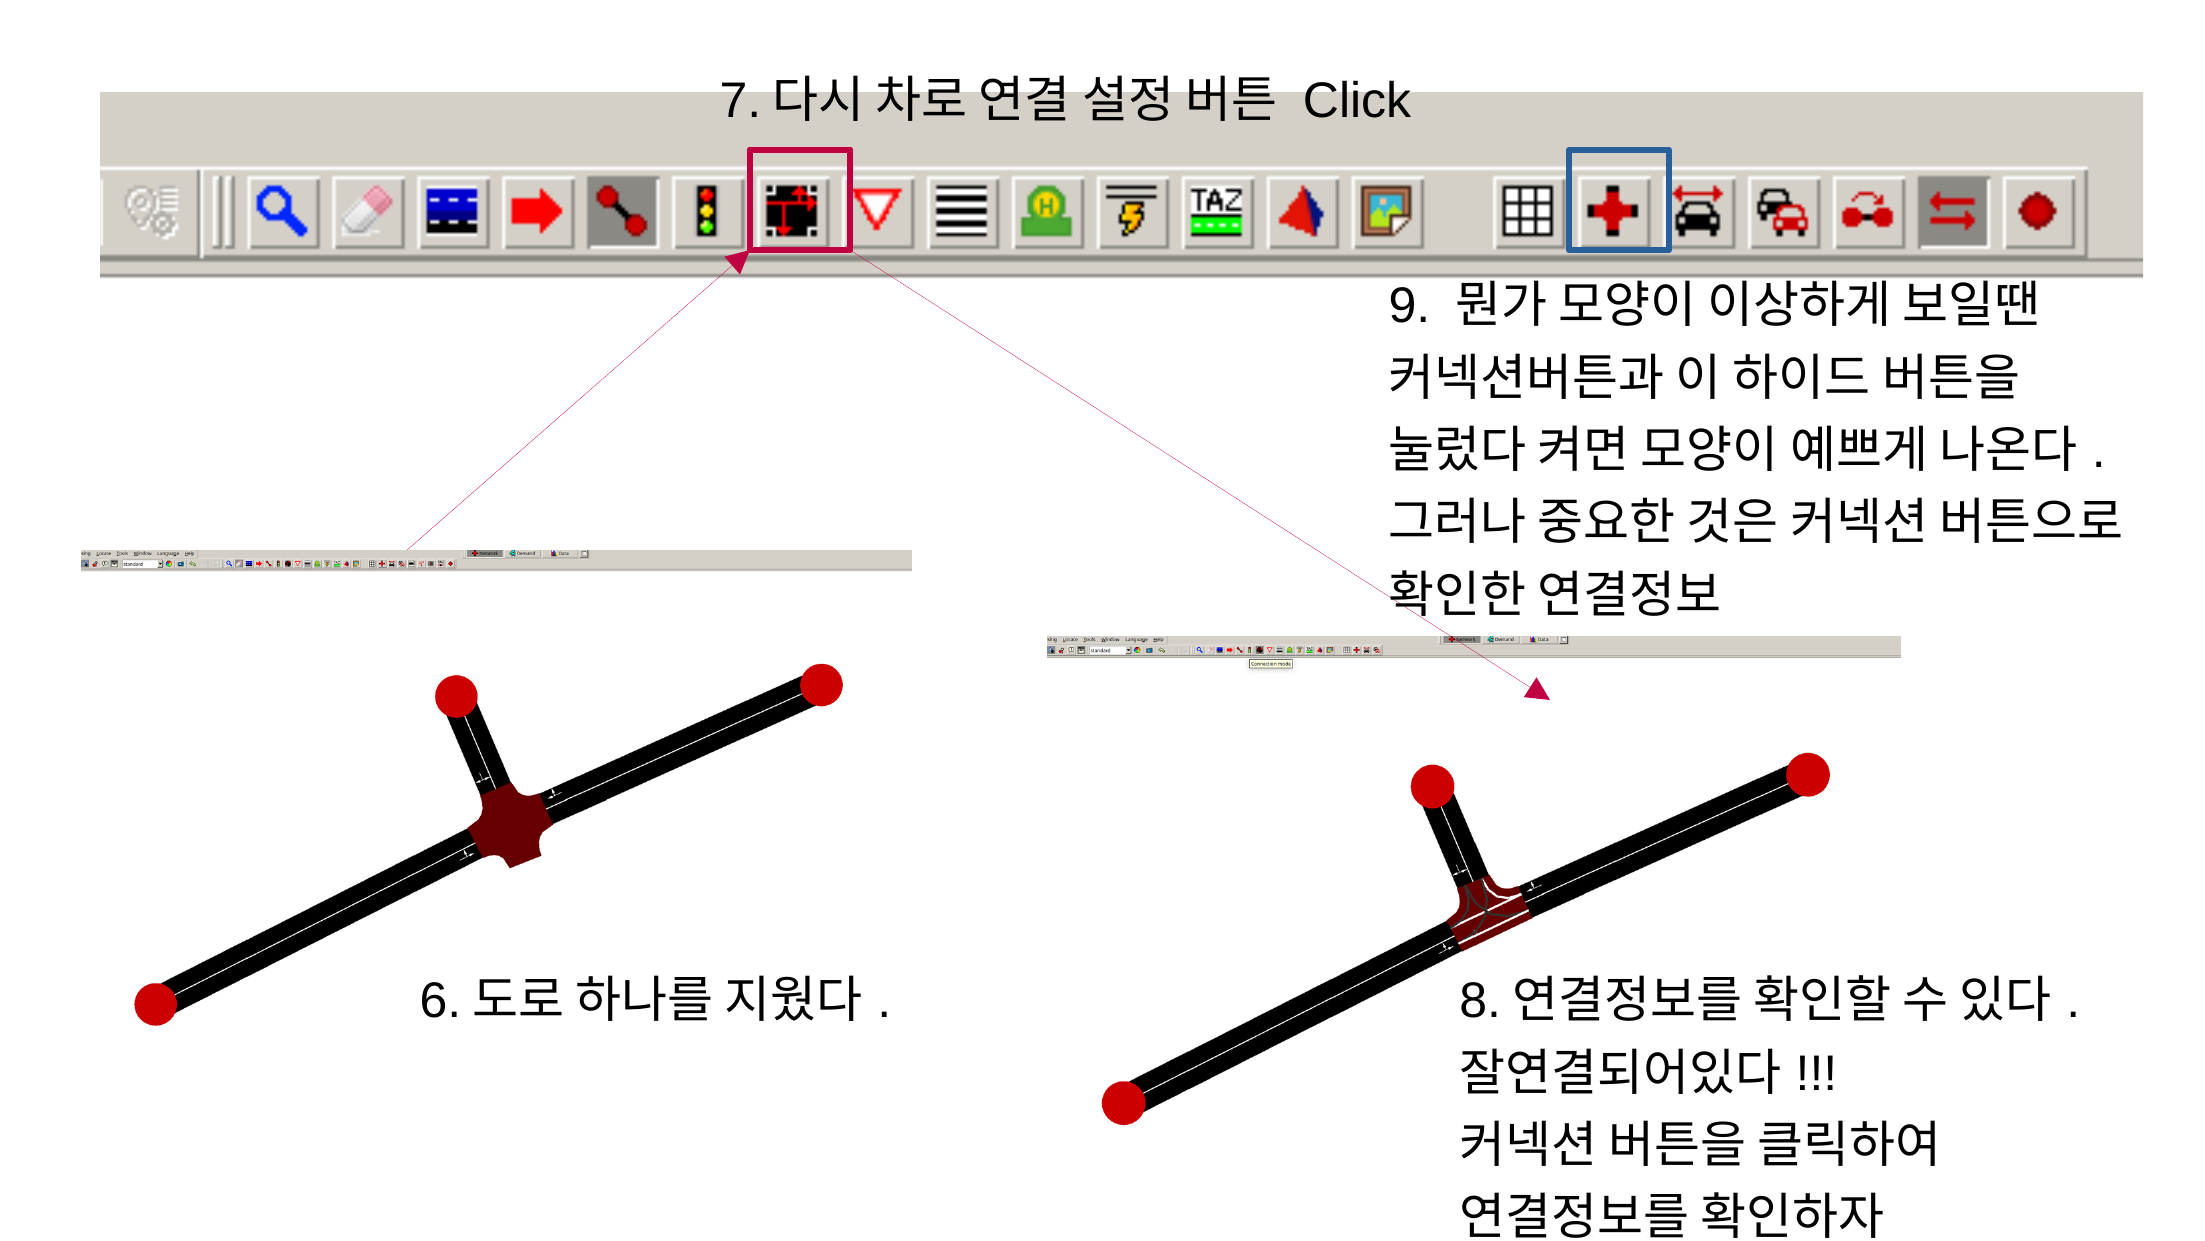
\includegraphics[keepaspectratio]{image/page-3.png}}

\bookmarksetup{startatroot}

\chapter{SUMO 자습 자료}\label{sumo-uxc790uxc2b5-uxc790uxb8cc}

\begin{itemize}
\item
  \href{https://sumo.dlr.de/docs/Tutorials/index.html}{sumo 공식
  튜토리얼}
\item
  \href{https://sumo.dlr.de/docs/index.html}{sumo 도큐먼트}
\item
  잘 설명된 한국어 블로그
  \href{https://treesparrow.tistory.com/9}{교통앵무}
\item
  잘 설명해주는 Youtube 채널
  \href{https://youtu.be/vANQ6eitfnw?si=WAAx6MG-Lhv0z46L}{KnowMaga}
\end{itemize}

\bookmarksetup{startatroot}

\chapter{이메일 문의}\label{uxc774uxba54uxc77c-uxbb38uxc758}

아래와 같이 문의 주시면, 문제 해결에 도움이 됩니다.

문의 주소 : yoonim98@hanyang.ac.kr 이메일 제목 : {[}교통공학 -SUMO{]}
이름(학과, 학번) 문의 이메일 내용 필수 포함 사항

\begin{itemize}
\tightlist
\item
  운영체제
\item
  질문
\item
  스크린 샷
\item
  문제파일, 폴더 등
\end{itemize}

\pandocbounded{\includegraphics[keepaspectratio]{image/page-42.pdf}}

\protect\phantomsection\label{refs}
\begin{CSLReferences}{1}{1}
\bibitem[\citeproctext]{ref-lopezMicroscopicTrafficSimulation2018}
Lopez, Pablo Alvarez, Michael Behrisch, Laura Bieker-Walz, et al. 2018.
{``{Microscopic Traffic Simulation using SUMO}.''} \emph{{2018 21st
International Conference on Intelligent Transportation Systems (ITSC)}},
January, 2575--82. \url{https://doi.org/10.1109/ITSC.2018.8569938}.

\end{CSLReferences}




\end{document}
